\documentclass[]{book}
\usepackage{lmodern}
\usepackage{amssymb,amsmath}
\usepackage{ifxetex,ifluatex}
\usepackage{fixltx2e} % provides \textsubscript
\ifnum 0\ifxetex 1\fi\ifluatex 1\fi=0 % if pdftex
  \usepackage[T1]{fontenc}
  \usepackage[utf8]{inputenc}
\else % if luatex or xelatex
  \ifxetex
    \usepackage{mathspec}
  \else
    \usepackage{fontspec}
  \fi
  \defaultfontfeatures{Ligatures=TeX,Scale=MatchLowercase}
\fi
% use upquote if available, for straight quotes in verbatim environments
\IfFileExists{upquote.sty}{\usepackage{upquote}}{}
% use microtype if available
\IfFileExists{microtype.sty}{%
\usepackage{microtype}
\UseMicrotypeSet[protrusion]{basicmath} % disable protrusion for tt fonts
}{}
\usepackage{hyperref}
\hypersetup{unicode=true,
            pdftitle={Applications of Machine Learning in Imputation},
            pdfauthor={Vinayak Anand-Kumar},
            pdfborder={0 0 0},
            breaklinks=true}
\urlstyle{same}  % don't use monospace font for urls
\usepackage{natbib}
\bibliographystyle{apalike}
\usepackage{color}
\usepackage{fancyvrb}
\newcommand{\VerbBar}{|}
\newcommand{\VERB}{\Verb[commandchars=\\\{\}]}
\DefineVerbatimEnvironment{Highlighting}{Verbatim}{commandchars=\\\{\}}
% Add ',fontsize=\small' for more characters per line
\usepackage{framed}
\definecolor{shadecolor}{RGB}{248,248,248}
\newenvironment{Shaded}{\begin{snugshade}}{\end{snugshade}}
\newcommand{\KeywordTok}[1]{\textcolor[rgb]{0.13,0.29,0.53}{\textbf{#1}}}
\newcommand{\DataTypeTok}[1]{\textcolor[rgb]{0.13,0.29,0.53}{#1}}
\newcommand{\DecValTok}[1]{\textcolor[rgb]{0.00,0.00,0.81}{#1}}
\newcommand{\BaseNTok}[1]{\textcolor[rgb]{0.00,0.00,0.81}{#1}}
\newcommand{\FloatTok}[1]{\textcolor[rgb]{0.00,0.00,0.81}{#1}}
\newcommand{\ConstantTok}[1]{\textcolor[rgb]{0.00,0.00,0.00}{#1}}
\newcommand{\CharTok}[1]{\textcolor[rgb]{0.31,0.60,0.02}{#1}}
\newcommand{\SpecialCharTok}[1]{\textcolor[rgb]{0.00,0.00,0.00}{#1}}
\newcommand{\StringTok}[1]{\textcolor[rgb]{0.31,0.60,0.02}{#1}}
\newcommand{\VerbatimStringTok}[1]{\textcolor[rgb]{0.31,0.60,0.02}{#1}}
\newcommand{\SpecialStringTok}[1]{\textcolor[rgb]{0.31,0.60,0.02}{#1}}
\newcommand{\ImportTok}[1]{#1}
\newcommand{\CommentTok}[1]{\textcolor[rgb]{0.56,0.35,0.01}{\textit{#1}}}
\newcommand{\DocumentationTok}[1]{\textcolor[rgb]{0.56,0.35,0.01}{\textbf{\textit{#1}}}}
\newcommand{\AnnotationTok}[1]{\textcolor[rgb]{0.56,0.35,0.01}{\textbf{\textit{#1}}}}
\newcommand{\CommentVarTok}[1]{\textcolor[rgb]{0.56,0.35,0.01}{\textbf{\textit{#1}}}}
\newcommand{\OtherTok}[1]{\textcolor[rgb]{0.56,0.35,0.01}{#1}}
\newcommand{\FunctionTok}[1]{\textcolor[rgb]{0.00,0.00,0.00}{#1}}
\newcommand{\VariableTok}[1]{\textcolor[rgb]{0.00,0.00,0.00}{#1}}
\newcommand{\ControlFlowTok}[1]{\textcolor[rgb]{0.13,0.29,0.53}{\textbf{#1}}}
\newcommand{\OperatorTok}[1]{\textcolor[rgb]{0.81,0.36,0.00}{\textbf{#1}}}
\newcommand{\BuiltInTok}[1]{#1}
\newcommand{\ExtensionTok}[1]{#1}
\newcommand{\PreprocessorTok}[1]{\textcolor[rgb]{0.56,0.35,0.01}{\textit{#1}}}
\newcommand{\AttributeTok}[1]{\textcolor[rgb]{0.77,0.63,0.00}{#1}}
\newcommand{\RegionMarkerTok}[1]{#1}
\newcommand{\InformationTok}[1]{\textcolor[rgb]{0.56,0.35,0.01}{\textbf{\textit{#1}}}}
\newcommand{\WarningTok}[1]{\textcolor[rgb]{0.56,0.35,0.01}{\textbf{\textit{#1}}}}
\newcommand{\AlertTok}[1]{\textcolor[rgb]{0.94,0.16,0.16}{#1}}
\newcommand{\ErrorTok}[1]{\textcolor[rgb]{0.64,0.00,0.00}{\textbf{#1}}}
\newcommand{\NormalTok}[1]{#1}
\usepackage{longtable,booktabs}
\usepackage{graphicx,grffile}
\makeatletter
\def\maxwidth{\ifdim\Gin@nat@width>\linewidth\linewidth\else\Gin@nat@width\fi}
\def\maxheight{\ifdim\Gin@nat@height>\textheight\textheight\else\Gin@nat@height\fi}
\makeatother
% Scale images if necessary, so that they will not overflow the page
% margins by default, and it is still possible to overwrite the defaults
% using explicit options in \includegraphics[width, height, ...]{}
\setkeys{Gin}{width=\maxwidth,height=\maxheight,keepaspectratio}
\IfFileExists{parskip.sty}{%
\usepackage{parskip}
}{% else
\setlength{\parindent}{0pt}
\setlength{\parskip}{6pt plus 2pt minus 1pt}
}
\setlength{\emergencystretch}{3em}  % prevent overfull lines
\providecommand{\tightlist}{%
  \setlength{\itemsep}{0pt}\setlength{\parskip}{0pt}}
\setcounter{secnumdepth}{5}
% Redefines (sub)paragraphs to behave more like sections
\ifx\paragraph\undefined\else
\let\oldparagraph\paragraph
\renewcommand{\paragraph}[1]{\oldparagraph{#1}\mbox{}}
\fi
\ifx\subparagraph\undefined\else
\let\oldsubparagraph\subparagraph
\renewcommand{\subparagraph}[1]{\oldsubparagraph{#1}\mbox{}}
\fi

%%% Use protect on footnotes to avoid problems with footnotes in titles
\let\rmarkdownfootnote\footnote%
\def\footnote{\protect\rmarkdownfootnote}

%%% Change title format to be more compact
\usepackage{titling}

% Create subtitle command for use in maketitle
\providecommand{\subtitle}[1]{
  \posttitle{
    \begin{center}\large#1\end{center}
    }
}

\setlength{\droptitle}{-2em}

  \title{Applications of Machine Learning in Imputation}
    \pretitle{\vspace{\droptitle}\centering\huge}
  \posttitle{\par}
    \author{Vinayak Anand-Kumar}
    \preauthor{\centering\large\emph}
  \postauthor{\par}
      \predate{\centering\large\emph}
  \postdate{\par}
    \date{2019}

\usepackage{booktabs}
\usepackage{amsthm}
\makeatletter
\def\thm@space@setup{%
  \thm@preskip=8pt plus 2pt minus 4pt
  \thm@postskip=\thm@preskip
}
\makeatother

\begin{document}
\maketitle

{
\setcounter{tocdepth}{1}
\tableofcontents
}
\chapter{Introduction}\label{introduction}

Editing and imputation are both methods of data processing. Editing
refers to the detection and correction of errors in the data, whilst
imputation is a method of correcting errors in a dataset. This document
presents findings from work carried out on the use of machine learning
in imputation. The chapters address the following questions:

\begin{enumerate}
\def\labelenumi{\arabic{enumi})}
\tightlist
\item
  What is imputation?\\
\item
  What is machine learning?\\
\item
  Why use machine learning?\\
\item
  How XGBoost works?\\
\item
  Methods used for the investigation\\
\item
  Results of the investigation\\
\item
  Conclusions and future direction
\end{enumerate}

\chapter{What is Imputation?}\label{what-is-imputation}

Editing and imputing are both methods of data processing. Editing refers
to the detection and correction of errors in the data. Whilst imputation
is a method of correcting errors and estimating and filling in missing
values in a data set. Where there are errors in the data set, and when
these are considered to add no value in the correction process, these
values are set to missing and are imputed with a plausible estimate.
Alternatively, missing values may already exist in the data, and
imputation may be carried out to produce a complete data set for
analysis.

This research project evaluated the use of machine learning methods for
imputation. In order to provide a context for using machine learning in
the imputation process, the reader is presented with:

\begin{itemize}
\tightlist
\item
  A rationale for carrying out imputation\\
\item
  An introduction to the methods of imputation
\end{itemize}

\section{Why is imputation carried
out?}\label{why-is-imputation-carried-out}

Missingness and erroneous values can impact the quality of data. A large
volume of incorrect and/or missing values increase the risk of the
product failing to capture the target concept or target population. That
is, omissions (introduced in collection or processing) may result in
certain sub-groups of the target population from being excluded in the
analysis data set, and in turn increasing the risk of biased estimates,
reducing the power of inferential statistics and increasing the
uncertainty of estimates and inferences derived from the data.
Similarly, errors in a data set may impact the degree to which the final
estimate or output represents the reality it was designed to capture.

Correcting erroneous responses and filling in missing values helps
manage the quality of data. A complete data set can improve the accuracy
and reliability of estimates, and help maintain the consistency of
counts across published tables. Moreover, a data set with fewer errors
and more units may more accurately capture the underlying distribution
of the variable of interest. Selecting a method for estimating values in
a data set is generally advised by the nature of errors or missingness
in the data, and the output desired from the analysis data set.

\section{Methods}\label{methods}

An imputation process of a data set can be broken down into the
following three phases:

\begin{enumerate}
\def\labelenumi{\arabic{enumi})}
\tightlist
\item
  Review, whereby data is examined for potential problems; identifying
  instances of missingness and erroneous values\\
\item
  Select, whereby data is identified for further treatment. Of the
  potential problems identified in the review phase, a method is applied
  to determine which of these erroneous or missing cases need to be
  treated
\item
  Amend, whereby changes are applied to the data identified in the
  select phase by either correcting errors/ filling in missing values
\end{enumerate}

The focus of this project was in applying Machine Learning methods to
amend values in a data set. That is, it was of interest to compare
existing approaches, of treating missing or erroneous values by
estimating replacement figures, to machine learning methods. Methods of
variable amendment can be grouped into one of the following categories:

\begin{itemize}
\tightlist
\item
  interactive treatment\\
\item
  deductive imputation\\
\item
  model based imputation\\
\item
  donor based imputation
\end{itemize}

The mechanisms for a given imputation method could be deterministic or
stochastic. The former refers to instances where repeated trials of the
same method yield identical output. Whereas the latter refers to
instances where there is element of randomness; repeated iterations will
produce different results.

\subsection{Interactive treatment}\label{interactive-treatment}

Interactive treatment refers to a class of methods whereby the data are
adjusted by a human editor by either re-contacting the respondent/ data
provider, replacing values from another variable/ data source, or
creating a value based on subject matter expertise.

\subsection{Deductive imputation}\label{deductive-imputation}

Deductive imputation uses logic or an understanding about the
relationship between variables and units to fill in missing values.
Examples include deriving a value as a function of other values,
adopting a value from a related unit, and adopting a value from an
earlier time point. Generally, this method is used when the true value
can be derived with certainty or with a very high probability.

\subsection{Model based imputation}\label{model-based-imputation}

Model based imputation refers to a class of methods that estimate
missing values using assumptions about the distribution of the data,
which include mean and median imputation. Or assumptions about the
relationship between auxiliary variables (or x variables) and the target
y variable to predict missing values.

\subsection{Donor based imputation}\label{donor-based-imputation}

Donor based imputation adopt values from an observed unit, which are
then used for the missing unit. For each recipient with a missing value
for variable y, a donor is identified that is similar to the recipient
with respect to certain background characteristics (often referred to as
matching variables) that are related to the target variable y. Such
methods are relatively easy to apply when there are several related
missing values in one record, and if the intention is to preserve the
relationship between variables.

\chapter{What is Machine Learning?}\label{what-is-machine-learning}

Machine learning is the field of study that enables a program to learn
from its experience of iterating through a task multiple times. A
performance measure is generally specified by the programmer, which is
used to evaluate how well the machine has carried out the task at each
iteration. Learning of the task is evidenced by its improvement against
the performance measure.\\
The different types of machine learning systems can be categorised with
respect to:

\begin{itemize}
\tightlist
\item
  Whether or not they are trained with human supervision\\
\item
  Whether or not they can learn incrementally or on the fly\\
\item
  Whether they work by comparing new data points to known data points,
  or instead detect patterns in the training data and build a predictive
  model
\end{itemize}

\section{Supervision}\label{supervision}

Machine learning systems can vary with regards to the degree of
supervision. The major types of supervision:

\begin{itemize}
\tightlist
\item
  Supervised learning\\
\item
  Unsupervised learning\\
\item
  Semi-supervised learning\\
\item
  Reinforcement learning
\end{itemize}

\subsection{Supervised learning}\label{supervised-learning}

Supervised learning is the specification of the desired output. That is,
the data used to train the model includes the solutions (which are
referred to as labels), which the machine learning system attempts to
estimate. The desired solutions specified in the machine learning
algorithm are referred to as labels.

\subsection{Unsupervised learning}\label{unsupervised-learning}

Unsupervised learning uses training data that is unlabelled. In this
class of machine learning systems, the outcome/ desired solutions are
not specified in the machine learning algorithm.

\subsection{Semi-supervised learning}\label{semi-supervised-learning}

Machine learning systems that use partially labelled data are
categorised as utilising semi-supervised learning.

\subsection{Reinforcement learning}\label{reinforcement-learning}

Reinforcement learning involves the use of rewards or penalties to train
the machine in identifying the appropriate action for a given situation.
The learning system, which is referred to as an agent, observes the
environment, selects and performs actions, and gets a response in the
form of a reward or penalty. After multiple iterations, it identifies
the best strategy, referred to as a policy, that results in the most
reward over time.

\section{Batch and Online learning}\label{batch-and-online-learning}

Another criterion for classifying machine learning systems is the way in
which the algorithm learns. That is, whether the learning takes place at
once or if it happens in increments.

\subsection{Batch learning}\label{batch-learning}

Batch learning uses all the available data to train the machine learning
system. This is generally time consuming and computationally expensive,
and as a result is carried out offline. Whilst in production, the system
is no longer learning, and is simply applying what it has learnt from
the full set of training data.

Any changes to the data generating mechanism (GDM) will mean that a new
system would need to be trained, from scratch on the full set of data
(that includes data points before and after changes to the GDM).

\subsection{Online learning}\label{online-learning}

Online learning trains the system incrementally through sequential input
of data. Data can be delivered individually or in small groups, referred
to as mini-batches. As each learning step is relatively fast and cheap,
the system can learn about new data whilst in production, as it arrives.
It is an ideal approach for when the velocity of new data is high, and
when there is a need to adapt to changes rapidly or autonomously.

\section{Approaches to
generalisation}\label{approaches-to-generalisation}

Machine learning systems can also be categorised with regards to how the
systems generalise. That is, there are different approaches to using the
training data to develop a system that can then be generalised to new
cases. The two main approaches are instance-based learning and
model-based learning.

\subsection{Instance-based learning}\label{instance-based-learning}

Instance-based learning identifies all instances of a given feature in
the training data and uses a similarity measure to generalise to new
cases.

\subsection{Model-based learning}\label{model-based-learning}

Model-based learning uses features in the training data to predict the
outcome/ variable of interest; the model used to specify the
relationship between the predictor(s) and outcome(s) are then
generalised on new cases.

\chapter{Why use Machine Learning?}\label{why-use-machine-learning}

It was of interest to explore the utility of Machine Learning to
directly impute for missing values in data sets. More specifically, the
analysts were interested in examining whether Machine Learning models
can improve the timeliness, reliability and accuracy of the imputation
process in social survey data. Figure 1 presents the imputation pipeline
for social survey data. Prior to imputation, units and values are
reviewed, and those that are missing and should be routed to the item in
question, are selected (i.e.~flagged) for imputation. Data is then
further processed before imputed and observed data are compiled in an
analysis data set, used for publishing estimates and carrying out
analyses.

\begin{figure}
\centering
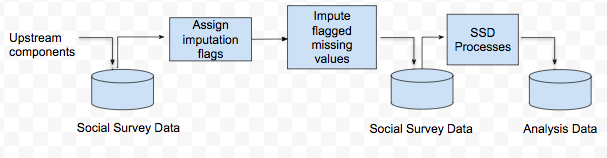
\includegraphics{images/CurrentPipeline.png}
\caption{Figure 1. Imputation pipeline in social survey data.}
\end{figure}

The intention was to use a machine learning system to impute flagged
missing values. This model based approach for imputation may reduce the
data processing time and improve the precision and reduce the variance
of estimates. The current approach, which utilises nearest neighbour
donor imputation involves the following:

\begin{itemize}
\tightlist
\item
  Setting up specification files for each variable and imputation group
  combination\\
\item
  Iterating through weights for matching variables so that all missing
  values are imputed
\end{itemize}

Designing the selection criteria for donors can be time consuming as it
requires analysts to identify matching variables (MV), along with
weights for each MV. Teams currently use subject matter expertise in
designing the donor imputation strategy for each variable. As this
process is not data driven, it introduces an element of subjectivity and
does not guarantee that matching variables selected are the best
predictors of the variable of interest. In contrast, a data driven
approach would be reproducible and identify the best predictors, in the
data set, to estimate missing values. Moreover, applying the machine
learning system may offer a more parsimonious approach as fewer input
parameters and files would be required in executing imputation.

Analysts were interested in whether a Machine Learning System would
perform better compared to the current imputation process with regards
to:

\begin{itemize}
\tightlist
\item
  Timeliness: Would the ML system reduce processing time and by how
  much?\\
\item
  Accuracy \& Reliability: How do the two methods compare with respect
  to the bias and variance of estimates?\\
\item
  Interpretability: What advantages and challenges do the ML system
  present with regards to making the imputation methods transparent?
\end{itemize}

At present, the following Machine Learning library was used in the
investigation:

\begin{itemize}
\tightlist
\item
  XGBoost
\end{itemize}

\chapter{XGBoost}\label{xgboost}

XGBoost is a set of open source functions and steps, referred to as a
library, that use supervised ML where analysts specify an outcome to be
estimated/ predicted. The XGBoost library uses multiple decision trees
to predict an outcome.

The ML system is trained using batch learning and generalised through a
model based approach. It uses all available data to construct a model
that specifies the relationship between the predictor and outcome
variables, which are then generalised to the test data set.

XGBoost stands for eXtreme Gradient Boosting. The word ``extreme''
reflects its goal to push the limit of computational resources. Whereas
gradient boosting is a machine learning technique for regression and
classification problems that optimises a collection of weak prediction
models in an attempt to build an accurate and reliable predictor.

In order to build a better understanding of how XGBoost works, the
documentation will briefly review:

\begin{itemize}
\tightlist
\item
  Decision trees: How decision trees play a role in XGBoost?\\
\item
  Boosting: What is it?
\end{itemize}

The final section of this chapter provides a step by step guide on
building models using XGBoost; the reader is encouraged to use this code
to predict an outcome variable using available auxiliary variables.

\section{Decision trees}\label{decision-trees}

Decision trees can be used as a method for grouping units in a data set
by asking questions, such as ``Does an individual have a Bachelor's
degree?''. In this example, two groups would be created; one for those
with a Bachelor's degree, and one for those without. Figure 2 provides a
visual depiction of this grouping in an attempt to explain Income.

\begin{figure}
\centering
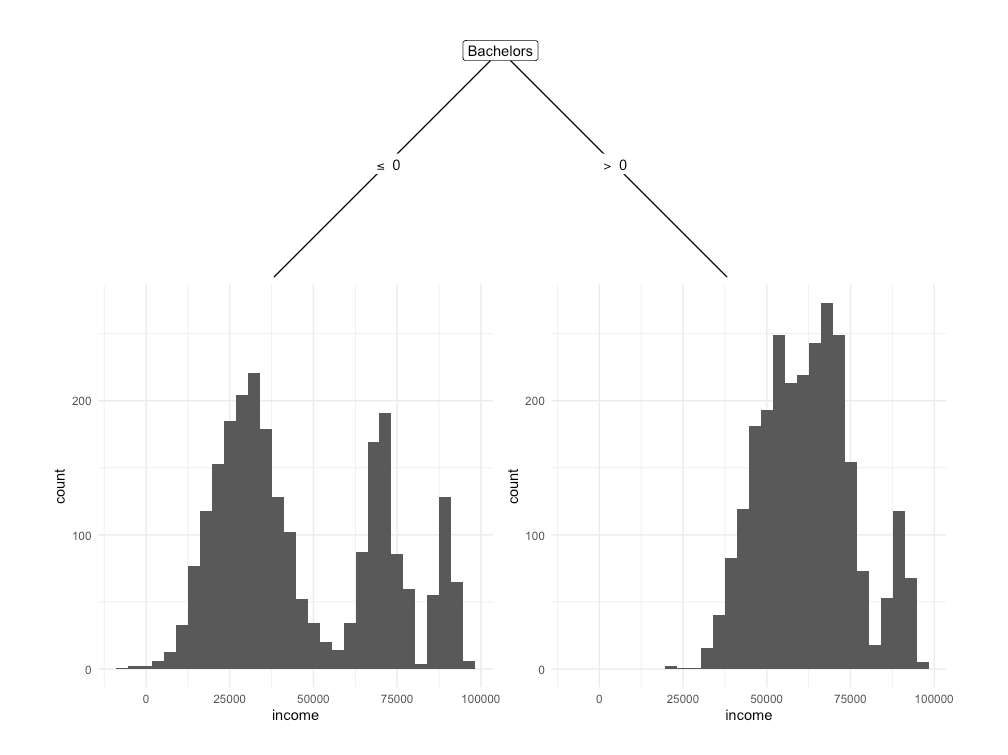
\includegraphics{images/dt_bach.png}
\caption{Figure 2. Decision tree that splits units in a dataset based on
whether individual has a Bachelor's degree or not, in order to predict
Income. The tree shows that those with a Bachelors degree
(\textgreater{} 0) on average earn more than than those wihtout a
Bachelor's degree (\textless{} 0).}
\end{figure}

Each subsequent question in a decision tree will produce a smaller group
of units. This grouping is carried out to identify units with similar
characteristics with respect to an outcome variable. The model in Figure
3 attempts to use University qualifications to predict Income.

\begin{figure}
\centering
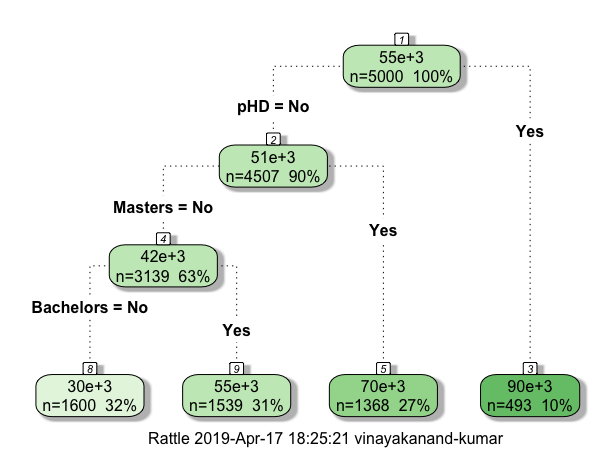
\includegraphics{images/dt_all.png}
\caption{Figure 3. Decision tree that splits units in a dataset based on
whether individual has a Bachelor's degree (yes/no), a Master's degree
and PhD (yes/no), in order to predict Income. The tree shows that those
with a higher qualification tend to earn more.}
\end{figure}

The following characteristics are true of decision trees:

\begin{itemize}
\tightlist
\item
  A single question is asked at each decision node, and there are only
  two possible choices. With the example in Figure 3, the questions
  include 1) Does the individual have a PhD, 2) Does the individual have
  a Master's and 3) Does the individual have a Bachelor's degree.\\
\item
  At the bottom of every decision tree, there is a single possible
  decision. Every possible decision will eventually lead to a choice.
  Some decisions will lead to a choice sooner. The model in Figure 3
  attempts to predict Income using University Qualifications. Each node
  presents a question about whether an individual possesses a given
  qualification. The end nodes present the distribution of income for
  individuals with the specified qualifications. As a result, the
  choices would be the expected value of Income for an individual, given
  the qualifications obtained.
\end{itemize}

Decision trees are a learning method that involve a tree like graph to
model either continuous or categorical choice given some data. It is
composed of a series of binary questions, which when answered in
succession yield a prediction about data at hand. XGBoost uses
Classification and Regression Trees (CART), which are presented in the
above examples, to predict the outcome variable.

\subsection{Boosting}\label{boosting}

A single decision tree is considered a weak/ base learner as it is only
slightly better than chance at predicting the outcome variable. Whereas
strong learners are any algorithm that can be tuned to achieve peak
performance for supervised learning. XGBoost uses decision trees as base
learners; combining many weak learners to form a strong learner. As a
result it is referred to as an ensemble learning method; using the
output of many models (i.e.~trees) in the final prediction.

The concept of combining many weak learners to produce a strong learner
is referred as boosting. XGBoost will iteratively build a set of weak
models on subsets of the data; weighting each weak prediction according
to the weak learner's performance. A prediction is derived by taking the
weighted sum of all base learners.

\subsection{Building models with
XGBoost}\label{building-models-with-xgboost}

In the training data, a target variable \(y_{i}\) is specified, whilst
all other features \(x_{i}\) are used as predictors of the target
variable. A collection of decision trees are used to predict values of
\(y_{i}\) using \(x_{i}\). Individually, each decision tree, would be a
weak predictor of the outcome variable. However, as a collective, the
decision trees may enable analysts to make accurate and reliable
predictions of \(y_{i}\). As a result, the method for predicting the
target variable using \(x_{i}\) in XGBoost is referred to as decision
tree ensembles. The steps below demonstrate how XGBoost was used to
build a model, to predict income, using University Qualifications.

\begin{enumerate}
\def\labelenumi{\arabic{enumi})}
\tightlist
\item
  Load the following packages
\end{enumerate}

\begin{Shaded}
\begin{Highlighting}[]
\KeywordTok{library}\NormalTok{(caret)}

\KeywordTok{library}\NormalTok{(xgboost)}
\end{Highlighting}
\end{Shaded}

\begin{enumerate}
\def\labelenumi{\arabic{enumi})}
\setcounter{enumi}{1}
\tightlist
\item
  Load the data set and remove the identifier
\end{enumerate}

\begin{Shaded}
\begin{Highlighting}[]
\CommentTok{# Load data}
\KeywordTok{load}\NormalTok{(}\StringTok{"data/Income_tree.RData"}\NormalTok{)}

\CommentTok{# Remove identifier}
\NormalTok{Income <-}\StringTok{ }\NormalTok{Income[,}\OperatorTok{-}\DecValTok{1}\NormalTok{]}
\end{Highlighting}
\end{Shaded}

\begin{enumerate}
\def\labelenumi{\arabic{enumi})}
\setcounter{enumi}{2}
\tightlist
\item
  Split the data set into training and test
\end{enumerate}

\begin{Shaded}
\begin{Highlighting}[]
\CommentTok{# Split data into training and test}
\KeywordTok{set.seed}\NormalTok{(}\DecValTok{5}\NormalTok{)}

\NormalTok{s <-}\StringTok{ }\KeywordTok{createDataPartition}\NormalTok{(Income}\OperatorTok{$}\NormalTok{income, }\DataTypeTok{p =} \FloatTok{0.8}\NormalTok{, }\DataTypeTok{list=}\OtherTok{FALSE}\NormalTok{)}

\NormalTok{training <-}\StringTok{ }\NormalTok{Income[s,]}

\NormalTok{test <-}\StringTok{ }\NormalTok{Income[}\OperatorTok{-}\NormalTok{s,]}
\end{Highlighting}
\end{Shaded}

\begin{enumerate}
\def\labelenumi{\arabic{enumi})}
\setcounter{enumi}{3}
\tightlist
\item
  Convert the data into DMatrix objects, which is the recommended input
  type for xgboost
\end{enumerate}

\begin{Shaded}
\begin{Highlighting}[]
\CommentTok{# Convert the data to matrix and assign output variable}
\NormalTok{train.outcome <-}\StringTok{ }\NormalTok{training}\OperatorTok{$}\NormalTok{income}

\NormalTok{train.predictors <-}\StringTok{ }\KeywordTok{sparse.model.matrix}\NormalTok{(income }\OperatorTok{~}\StringTok{ }\NormalTok{.,}
                                        \DataTypeTok{data =}\NormalTok{ training}
\NormalTok{)[, }\OperatorTok{-}\DecValTok{1}\NormalTok{]}

\NormalTok{test.outcome <-}\StringTok{ }\NormalTok{test}\OperatorTok{$}\NormalTok{income}

\NormalTok{test.predictors <-}\StringTok{ }\KeywordTok{model.matrix}\NormalTok{(income }\OperatorTok{~}\StringTok{ }\NormalTok{.,}
                                \DataTypeTok{data =}\NormalTok{ test}
\NormalTok{)[, }\OperatorTok{-}\DecValTok{1}\NormalTok{]}

\CommentTok{# Convert the matrix objects to DMatrix objects}
\NormalTok{dtrain <-}\StringTok{ }\KeywordTok{xgb.DMatrix}\NormalTok{(train.predictors, }\DataTypeTok{label=}\NormalTok{train.outcome)}

\NormalTok{dtest <-}\StringTok{ }\KeywordTok{xgb.DMatrix}\NormalTok{(test.predictors)}
\end{Highlighting}
\end{Shaded}

\begin{enumerate}
\def\labelenumi{\arabic{enumi})}
\setcounter{enumi}{4}
\tightlist
\item
  Train the model
\end{enumerate}

\begin{Shaded}
\begin{Highlighting}[]
\CommentTok{# Train the model}
\NormalTok{model <-}\StringTok{ }\KeywordTok{xgboost}\NormalTok{(}
  \DataTypeTok{data =}\NormalTok{ dtrain, }\DataTypeTok{max_depth =} \DecValTok{2}\NormalTok{, }\DataTypeTok{eta =} \DecValTok{1}\NormalTok{, }\DataTypeTok{nthread =} \DecValTok{2}\NormalTok{, }\DataTypeTok{nrounds =} \DecValTok{10}\NormalTok{,}
  \DataTypeTok{objective =} \StringTok{"reg:linear"}\NormalTok{)}
\end{Highlighting}
\end{Shaded}

\begin{enumerate}
\def\labelenumi{\arabic{enumi})}
\setcounter{enumi}{5}
\tightlist
\item
  Test the model
\end{enumerate}

\begin{Shaded}
\begin{Highlighting}[]
\CommentTok{# Test the model}
\NormalTok{pred <-}\StringTok{ }\KeywordTok{predict}\NormalTok{(model, dtest)}

\CommentTok{# Evaluate the performance of model}
\KeywordTok{RMSE}\NormalTok{(pred,test.outcome)}
\end{Highlighting}
\end{Shaded}

\begin{enumerate}
\def\labelenumi{\arabic{enumi})}
\setcounter{enumi}{6}
\tightlist
\item
  Examine the importance of each feature in the model
\end{enumerate}

\begin{Shaded}
\begin{Highlighting}[]
\CommentTok{# Examine feature importance}
\NormalTok{importance_matrix <-}\StringTok{ }\KeywordTok{xgb.importance}\NormalTok{(}\DataTypeTok{model =}\NormalTok{ model)}

\KeywordTok{print}\NormalTok{(importance_matrix)}

\KeywordTok{xgb.plot.importance}\NormalTok{(}\DataTypeTok{importance_matrix =}\NormalTok{ importance_matrix)}
\end{Highlighting}
\end{Shaded}

\begin{enumerate}
\def\labelenumi{\arabic{enumi})}
\setcounter{enumi}{7}
\tightlist
\item
  Plot the individual trees in the model
\end{enumerate}

\begin{Shaded}
\begin{Highlighting}[]
\CommentTok{# Plot the trees}
\CommentTok{# Tree 1}
\KeywordTok{xgb.plot.tree}\NormalTok{(}\DataTypeTok{model =}\NormalTok{ model, }\DataTypeTok{tree=}\DecValTok{0}\NormalTok{)}
\CommentTok{# Tree 2}
\KeywordTok{xgb.plot.tree}\NormalTok{(}\DataTypeTok{model =}\NormalTok{ model, }\DataTypeTok{tree=}\DecValTok{1}\NormalTok{)}
\CommentTok{# Tree 3}
\KeywordTok{xgb.plot.tree}\NormalTok{(}\DataTypeTok{model =}\NormalTok{ model, }\DataTypeTok{tree=}\DecValTok{2}\NormalTok{)}
\end{Highlighting}
\end{Shaded}

\chapter{Methods}\label{methods-1}

The project evaluated the machine learning methods using:

\begin{enumerate}
\def\labelenumi{\arabic{enumi})}
\tightlist
\item
  The Census Teaching File, an open data set containing 1\% of the
  person records from the 2011 Census in England \& Wales.\\
\item
  Survey Data
\end{enumerate}

\section{Census Teaching File}\label{census-teaching-file}

The Census Teaching File was downloaded from the
\href{https://www.ons.gov.uk/census/2011census/2011censusdata/censusmicrodata/microdatateachingfile}{ONS
website} as a CSV file named ``CensusTeachingFile'', and was read into R
using the following line of code. The data set consisted of 569,741
individuals and 18 categorical variables from the 2011 Census
population.

\begin{Shaded}
\begin{Highlighting}[]
\CommentTok{# Read CSV into R}
\NormalTok{CensusRaw <-}\StringTok{ }\KeywordTok{read.csv}\NormalTok{(}
  \DataTypeTok{file =} \StringTok{"data/source/CensusTeachingFile.csv"}\NormalTok{, }\DataTypeTok{skip =} \DecValTok{1}\NormalTok{,}
  \DataTypeTok{header =} \OtherTok{TRUE}\NormalTok{, }\DataTypeTok{sep =} \StringTok{","}
\NormalTok{)}
\end{Highlighting}
\end{Shaded}

The code below specifies the packages used in the preparation, study and
build of machine learning systems using the Census Teaching File.

\begin{Shaded}
\begin{Highlighting}[]
\KeywordTok{library}\NormalTok{(tidyverse)}
\KeywordTok{library}\NormalTok{(mice)}
\KeywordTok{library}\NormalTok{(reshape2)}
\KeywordTok{library}\NormalTok{(GGally)}
\KeywordTok{library}\NormalTok{(Matrix)}
\KeywordTok{library}\NormalTok{(xgboost)}
\KeywordTok{library}\NormalTok{(caret)}
\KeywordTok{library}\NormalTok{(DiagrammeR)}
\KeywordTok{library}\NormalTok{(MLmetrics)}
\KeywordTok{library}\NormalTok{(rpart)}
\KeywordTok{library}\NormalTok{(scales)}
\KeywordTok{library}\NormalTok{(knitr)}
\KeywordTok{library}\NormalTok{(kableExtra)}
\KeywordTok{library}\NormalTok{(DescTools)}
\KeywordTok{library}\NormalTok{(dummies)}
\end{Highlighting}
\end{Shaded}

The steps below present the methods used to compare the performance of
model based imputation (using XGBoost) with that of donor based
imputation (using CANCEIS). Code chunks are provided to demonstrate how
each step was carried out; with the imputable variable, economic
activity, as the example.

\begin{enumerate}
\def\labelenumi{\arabic{enumi})}
\tightlist
\item
  Variables in the data set were renamed and recoded so that:
\end{enumerate}

\begin{itemize}
\tightlist
\item
  Variable names were consistent with
  \href{https://google.github.io/styleguide/Rguide.xml}{Google's R style
  guide}
\item
  The response categories for all variables were numeric
\end{itemize}

\begin{Shaded}
\begin{Highlighting}[]
\CommentTok{# Rename variables}
\NormalTok{Census <-}\StringTok{ }\NormalTok{plyr}\OperatorTok{::}\KeywordTok{rename}\NormalTok{(CensusRaw, }\KeywordTok{c}\NormalTok{(}
  \StringTok{"Person.ID"}\NormalTok{ =}\StringTok{ "person.id"}\NormalTok{,}
  \StringTok{"Region"}\NormalTok{ =}\StringTok{ "region"}\NormalTok{,}
  \StringTok{"Residence.Type"}\NormalTok{ =}\StringTok{ "residence.type"}\NormalTok{,}
  \StringTok{"Family.Composition"}\NormalTok{ =}\StringTok{ "fam.comp"}\NormalTok{,}
  \StringTok{"Population.Base"}\NormalTok{ =}\StringTok{ "resident.type"}\NormalTok{,}
  \StringTok{"Sex"}\NormalTok{ =}\StringTok{ "sex"}\NormalTok{,}
  \StringTok{"Age"}\NormalTok{ =}\StringTok{ "age"}\NormalTok{,}
  \StringTok{"Marital.Status"}\NormalTok{ =}\StringTok{ "marital.status"}\NormalTok{,}
  \StringTok{"Student"}\NormalTok{ =}\StringTok{ "student"}\NormalTok{,}
  \StringTok{"Country.of.Birth"}\NormalTok{ =}\StringTok{ "birth.country"}\NormalTok{,}
  \StringTok{"Health"}\NormalTok{ =}\StringTok{ "health"}\NormalTok{,}
  \StringTok{"Ethnic.Group"}\NormalTok{ =}\StringTok{ "ethnicity"}\NormalTok{,}
  \StringTok{"Religion"}\NormalTok{ =}\StringTok{ "religion"}\NormalTok{,}
  \StringTok{"Economic.Activity"}\NormalTok{ =}\StringTok{ "econ.act"}\NormalTok{,}
  \StringTok{"Occupation"}\NormalTok{ =}\StringTok{ "occupation"}\NormalTok{,}
  \StringTok{"Industry"}\NormalTok{ =}\StringTok{ "industry"}\NormalTok{,}
  \StringTok{"Hours.worked.per.week"}\NormalTok{ =}\StringTok{ "hours.worked"}\NormalTok{,}
  \StringTok{"Approximated.Social.Grade"}\NormalTok{ =}\StringTok{ "social.grade"}
\NormalTok{))}

\CommentTok{# Recode variables (dataset is mutated in order to recode variables)}
\NormalTok{Census <-}\StringTok{ }\NormalTok{Census }\OperatorTok\StringTok{ }\KeywordTok{mutate_if}\NormalTok{(is.factor, as.character)}

\CommentTok{# Recode the Region variable so that it is numeric}
\NormalTok{Census}\OperatorTok{$}\NormalTok{region[Census}\OperatorTok{$}\NormalTok{region }\OperatorTok{==}\StringTok{ "E12000001"}\NormalTok{] <-}\StringTok{ }\DecValTok{1}
\NormalTok{Census}\OperatorTok{$}\NormalTok{region[Census}\OperatorTok{$}\NormalTok{region }\OperatorTok{==}\StringTok{ "E12000002"}\NormalTok{] <-}\StringTok{ }\DecValTok{2}
\NormalTok{Census}\OperatorTok{$}\NormalTok{region[Census}\OperatorTok{$}\NormalTok{region }\OperatorTok{==}\StringTok{ "E12000003"}\NormalTok{] <-}\StringTok{ }\DecValTok{3}
\NormalTok{Census}\OperatorTok{$}\NormalTok{region[Census}\OperatorTok{$}\NormalTok{region }\OperatorTok{==}\StringTok{ "E12000004"}\NormalTok{] <-}\StringTok{ }\DecValTok{4}
\NormalTok{Census}\OperatorTok{$}\NormalTok{region[Census}\OperatorTok{$}\NormalTok{region }\OperatorTok{==}\StringTok{ "E12000005"}\NormalTok{] <-}\StringTok{ }\DecValTok{5}
\NormalTok{Census}\OperatorTok{$}\NormalTok{region[Census}\OperatorTok{$}\NormalTok{region }\OperatorTok{==}\StringTok{ "E12000006"}\NormalTok{] <-}\StringTok{ }\DecValTok{6}
\NormalTok{Census}\OperatorTok{$}\NormalTok{region[Census}\OperatorTok{$}\NormalTok{region }\OperatorTok{==}\StringTok{ "E12000007"}\NormalTok{] <-}\StringTok{ }\DecValTok{7}
\NormalTok{Census}\OperatorTok{$}\NormalTok{region[Census}\OperatorTok{$}\NormalTok{region }\OperatorTok{==}\StringTok{ "E12000008"}\NormalTok{] <-}\StringTok{ }\DecValTok{8}
\NormalTok{Census}\OperatorTok{$}\NormalTok{region[Census}\OperatorTok{$}\NormalTok{region }\OperatorTok{==}\StringTok{ "E12000009"}\NormalTok{] <-}\StringTok{ }\DecValTok{9}
\NormalTok{Census}\OperatorTok{$}\NormalTok{region[Census}\OperatorTok{$}\NormalTok{region }\OperatorTok{==}\StringTok{ "W92000004"}\NormalTok{] <-}\StringTok{ }\DecValTok{10}

\NormalTok{Census}\OperatorTok{$}\NormalTok{residence.type[Census}\OperatorTok{$}\NormalTok{residence.type }\OperatorTok{==}\StringTok{ "C"}\NormalTok{] <-}\StringTok{ }\DecValTok{0}
\NormalTok{Census}\OperatorTok{$}\NormalTok{residence.type[Census}\OperatorTok{$}\NormalTok{residence.type }\OperatorTok{==}\StringTok{ "H"}\NormalTok{] <-}\StringTok{ }\DecValTok{1}

\NormalTok{Census}\OperatorTok{$}\NormalTok{student[Census}\OperatorTok{$}\NormalTok{student }\OperatorTok{==}\StringTok{ }\DecValTok{1}\NormalTok{] <-}\StringTok{ }\DecValTok{0}
\NormalTok{Census}\OperatorTok{$}\NormalTok{student[Census}\OperatorTok{$}\NormalTok{student }\OperatorTok{==}\StringTok{ }\DecValTok{2}\NormalTok{] <-}\StringTok{ }\DecValTok{1}

\NormalTok{Census}\OperatorTok{$}\NormalTok{sex[Census}\OperatorTok{$}\NormalTok{sex }\OperatorTok{==}\StringTok{ }\DecValTok{1}\NormalTok{] <-}\StringTok{ }\DecValTok{0}
\NormalTok{Census}\OperatorTok{$}\NormalTok{sex[Census}\OperatorTok{$}\NormalTok{sex }\OperatorTok{==}\StringTok{ }\DecValTok{2}\NormalTok{] <-}\StringTok{ }\DecValTok{1}

\NormalTok{Census}\OperatorTok{$}\NormalTok{birth.country[Census}\OperatorTok{$}\NormalTok{birth.country}\OperatorTok{==}\DecValTok{1}\NormalTok{] <-}\StringTok{ }\DecValTok{0}
\NormalTok{Census}\OperatorTok{$}\NormalTok{birth.country[Census}\OperatorTok{$}\NormalTok{birth.country}\OperatorTok{==}\DecValTok{2}\NormalTok{] <-}\StringTok{ }\DecValTok{1}

\NormalTok{Census <-}\StringTok{ }\NormalTok{Census }\OperatorTok\StringTok{ }\KeywordTok{mutate_if}\NormalTok{(is.character, as.numeric)}

\NormalTok{Census}\OperatorTok{$}\NormalTok{person.id <-}\StringTok{ }\KeywordTok{as.character}\NormalTok{(Census}\OperatorTok{$}\NormalTok{person.id)}

\NormalTok{Ht <-}\StringTok{ }\KeywordTok{table}\NormalTok{(Census}\OperatorTok{$}\NormalTok{hours.worked)}
\NormalTok{Census}\OperatorTok{$}\NormalTok{hours.cont <-}\StringTok{ }\KeywordTok{ifelse}\NormalTok{(Census}\OperatorTok{$}\NormalTok{hours.worked }\OperatorTok{==}\StringTok{ }\DecValTok{1}\NormalTok{, }\KeywordTok{runif}\NormalTok{(}
  \DecValTok{1}\OperatorTok{:}\NormalTok{Ht[}\KeywordTok{names}\NormalTok{(Ht) }\OperatorTok{==}\StringTok{ }\DecValTok{1}\NormalTok{],}
  \DecValTok{1}\NormalTok{, }\DecValTok{15}
\NormalTok{),}
\KeywordTok{ifelse}\NormalTok{(Census}\OperatorTok{$}\NormalTok{hours.worked }\OperatorTok{==}\StringTok{ }\DecValTok{2}\NormalTok{, }\KeywordTok{runif}\NormalTok{(}\DecValTok{1}\OperatorTok{:}\NormalTok{Ht[}\KeywordTok{names}\NormalTok{(Ht) }\OperatorTok{==}\StringTok{ }\DecValTok{2}\NormalTok{], }\DecValTok{16}\NormalTok{, }\DecValTok{30}\NormalTok{),}
  \KeywordTok{ifelse}\NormalTok{(Census}\OperatorTok{$}\NormalTok{hours.worked }\OperatorTok{==}\StringTok{ }\DecValTok{3}\NormalTok{, }\KeywordTok{runif}\NormalTok{(}\DecValTok{1}\OperatorTok{:}\NormalTok{Ht[}\KeywordTok{names}\NormalTok{(Ht) }\OperatorTok{==}\StringTok{ }\DecValTok{3}\NormalTok{], }\DecValTok{31}\NormalTok{, }\DecValTok{48}\NormalTok{),}
    \KeywordTok{ifelse}\NormalTok{(Census}\OperatorTok{$}\NormalTok{hours.worked }\OperatorTok{==}\StringTok{ }\DecValTok{4}\NormalTok{, }\KeywordTok{runif}\NormalTok{(}\DecValTok{1}\OperatorTok{:}\NormalTok{Ht[}\KeywordTok{names}\NormalTok{(Ht) }\OperatorTok{==}\StringTok{ }\DecValTok{4}\NormalTok{], }\DecValTok{49}\NormalTok{, }\DecValTok{60}\NormalTok{),}
\NormalTok{      Census}\OperatorTok{$}\NormalTok{hours.worked}
\NormalTok{    )}
\NormalTok{  )}
\NormalTok{)}
\NormalTok{)}

\KeywordTok{save}\NormalTok{(Census, }\DataTypeTok{file =} \StringTok{"data/core/Census.Rda"}\NormalTok{)}

\NormalTok{Census.pre.ohe <-}\StringTok{ }\NormalTok{Census}

\CommentTok{# Prepare Census data for one hot encoding}
\NormalTok{Census.pre.ohe}\OperatorTok{$}\NormalTok{fam.comp[Census.pre.ohe}\OperatorTok{$}\NormalTok{fam.comp }\OperatorTok{==}\StringTok{ }\OperatorTok{-}\DecValTok{9}\NormalTok{] <-}\StringTok{ "NCR"}

\NormalTok{Census.pre.ohe}\OperatorTok{$}\NormalTok{health[Census.pre.ohe}\OperatorTok{$}\NormalTok{health }\OperatorTok{==}\StringTok{ }\OperatorTok{-}\DecValTok{9}\NormalTok{] <-}\StringTok{ "NCR"}

\NormalTok{Census.pre.ohe}\OperatorTok{$}\NormalTok{ethnicity[Census.pre.ohe}\OperatorTok{$}\NormalTok{ethnicity }\OperatorTok{==}\StringTok{ }\OperatorTok{-}\DecValTok{9}\NormalTok{] <-}\StringTok{ "NCR"}

\NormalTok{Census.pre.ohe}\OperatorTok{$}\NormalTok{religion[Census.pre.ohe}\OperatorTok{$}\NormalTok{religion }\OperatorTok{==}\StringTok{ }\OperatorTok{-}\DecValTok{9}\NormalTok{] <-}\StringTok{ "NCR"}

\NormalTok{Census.pre.ohe}\OperatorTok{$}\NormalTok{econ.act[Census.pre.ohe}\OperatorTok{$}\NormalTok{econ.act }\OperatorTok{==}\StringTok{ }\OperatorTok{-}\DecValTok{9}\NormalTok{] <-}\StringTok{ "NCR"}

\NormalTok{Census.pre.ohe}\OperatorTok{$}\NormalTok{occupation[Census.pre.ohe}\OperatorTok{$}\NormalTok{occupation }\OperatorTok{==}\StringTok{ }\OperatorTok{-}\DecValTok{9}\NormalTok{] <-}\StringTok{ "NCR"}

\NormalTok{Census.pre.ohe}\OperatorTok{$}\NormalTok{industry[Census.pre.ohe}\OperatorTok{$}\NormalTok{industry }\OperatorTok{==}\StringTok{ }\OperatorTok{-}\DecValTok{9}\NormalTok{] <-}\StringTok{ "NCR"}

\NormalTok{Census.pre.ohe}\OperatorTok{$}\NormalTok{social.grade[Census.pre.ohe}\OperatorTok{$}\NormalTok{social.grade }\OperatorTok{==}\StringTok{ }\OperatorTok{-}\DecValTok{9}\NormalTok{] <-}\StringTok{ "NCR"}
\end{Highlighting}
\end{Shaded}

A preview of the data set is provided below.

person.id

region

residence.type

fam.comp

resident.type

sex

age

marital.status

student

birth.country

health

ethnicity

religion

econ.act

occupation

industry

hours.worked

social.grade

hours.cont

7394816

1

1

2

1

1

6

2

1

0

2

1

2

5

8

2

-9

4

-9.00000

7394745

1

1

5

1

0

4

1

1

0

1

1

2

1

8

6

4

3

52.97915

7395066

1

1

3

1

1

4

1

1

0

1

1

1

1

6

11

3

4

37.80685

7395329

1

1

3

1

1

2

1

1

0

2

1

2

1

7

7

3

2

39.52916

7394712

1

1

3

1

0

5

4

1

0

1

1

2

1

1

4

3

2

31.29265

7394750

1

1

2

1

0

6

2

1

0

2

1

1

1

9

2

3

3

31.04491

\begin{enumerate}
\def\labelenumi{\arabic{enumi})}
\setcounter{enumi}{1}
\tightlist
\item
  For the purposes of training and testing a machine learning system,
  the data was divided into training and test data sets using the
  following code.
\end{enumerate}

\begin{Shaded}
\begin{Highlighting}[]
\CommentTok{# Randomly select 80% of Census units and split into Train and Test data}
\KeywordTok{set.seed}\NormalTok{(}\DecValTok{5}\NormalTok{)}
\NormalTok{Census80 <-}\StringTok{ }\KeywordTok{sample}\NormalTok{(}\DecValTok{1}\OperatorTok{:}\KeywordTok{nrow}\NormalTok{(Census_ohe), }\FloatTok{0.8} \OperatorTok{*}\StringTok{ }\KeywordTok{nrow}\NormalTok{(Census_ohe), }\DataTypeTok{replace =} \OtherTok{FALSE}\NormalTok{)}
\NormalTok{Census20 <-}\StringTok{ }\KeywordTok{setdiff}\NormalTok{(}\DecValTok{1}\OperatorTok{:}\KeywordTok{nrow}\NormalTok{(Census_ohe), Census80)}

\NormalTok{Census.train.ohe <-}\StringTok{ }\NormalTok{Census_ohe[Census80, }\OperatorTok{!}\NormalTok{(}\KeywordTok{names}\NormalTok{(Census_ohe)}\OperatorTok{==}\StringTok{"hours.worked"}\NormalTok{)]}
\NormalTok{Census.test.ohe <-}\StringTok{ }\NormalTok{Census_ohe[Census20, }\OperatorTok{!}\NormalTok{(}\KeywordTok{names}\NormalTok{(Census_ohe)}\OperatorTok{==}\StringTok{"hours.worked"}\NormalTok{)]}

\NormalTok{Census.train.label <-}\StringTok{ }\NormalTok{Census[Census80, }\OperatorTok{!}\NormalTok{(}\KeywordTok{names}\NormalTok{(Census)}\OperatorTok{==}\StringTok{"hours.worked"}\NormalTok{)]}
\NormalTok{Census.test.label <-}\StringTok{ }\NormalTok{Census[Census20, }\OperatorTok{!}\NormalTok{(}\KeywordTok{names}\NormalTok{(Census)}\OperatorTok{==}\StringTok{"hours.worked"}\NormalTok{)]}

\KeywordTok{save}\NormalTok{(Census.train.ohe, }\DataTypeTok{file =} \StringTok{"data/ohe/Census.train.ohe.Rda"}\NormalTok{)}
\KeywordTok{save}\NormalTok{(Census.test.ohe, }\DataTypeTok{file =} \StringTok{"data/ohe/Census.test.ohe.Rda"}\NormalTok{)}

\KeywordTok{save}\NormalTok{(Census.train.label, }\DataTypeTok{file =} \StringTok{"data/label/Census.train.label.Rda"}\NormalTok{)}
\KeywordTok{save}\NormalTok{(Census.test.label, }\DataTypeTok{file =} \StringTok{"data/label/Census.test.label.Rda"}\NormalTok{)}
\end{Highlighting}
\end{Shaded}

The intention was to build models to predict a selection of variable
using training data, which had no missingness. This model would then be
evaluated with respect to its accuracy and generalisability using a test
data set, which would have missingness. The Census Teaching File was a
complete data set. As a result, missingness was simulated in the test
data set, and the imputation models (derived for each variable) were
evaluated with regards to how well they predicted the true values.

Models were tested for the following variables:\\
- Economic activity (a multi-class variable) - Hours worked (a derived
continuous variable)\\
- Social Grade (a multi-class variable)\\
- Student status (a binary variable) A more detailed description of all
the variables can be found
\href{https://www.ons.gov.uk/census/2011census/2011censusdata/censusmicrodata/microdatateachingfile/variablelist}{here}.

\begin{enumerate}
\def\labelenumi{\arabic{enumi})}
\setcounter{enumi}{2}
\tightlist
\item
  The distribution of the imputable variable was studied
\end{enumerate}

\begin{Shaded}
\begin{Highlighting}[]
\CommentTok{# Study the variable: How many units in each category?}
\NormalTok{EAt <-}\StringTok{ }\KeywordTok{table}\NormalTok{(Census}\OperatorTok{$}\NormalTok{econ.act)}

\NormalTok{EAt}

\CommentTok{# What is the distribution of the variable: Remove NCR and plot to look at distribution}
\NormalTok{g <-}\StringTok{ }\KeywordTok{ggplot}\NormalTok{(Census[}\OperatorTok{!}\NormalTok{Census}\OperatorTok{$}\NormalTok{econ.act }\OperatorTok{==}\StringTok{ }\OperatorTok{-}\DecValTok{9}\NormalTok{, ], }\KeywordTok{aes}\NormalTok{(econ.act))}

\NormalTok{g }\OperatorTok{+}\StringTok{ }\KeywordTok{geom_bar}\NormalTok{() }\OperatorTok{+}\StringTok{ }\KeywordTok{scale_x_discrete}\NormalTok{(}
  \DataTypeTok{name =} \StringTok{"Economic Activity"}\NormalTok{,}
  \DataTypeTok{breaks =} \KeywordTok{pretty_breaks}\NormalTok{()}
\NormalTok{)}
\end{Highlighting}
\end{Shaded}

\begin{enumerate}
\def\labelenumi{\arabic{enumi})}
\setcounter{enumi}{3}
\item
  The data set was cleaned for model training; the personal identifier
  and the categorical hours worked variable were removed. Moreover,
  units that were classified as no code required for the imputable
  variable were removed from the training and test data sets
\item
  Missingness was simulated in the test data set
\end{enumerate}

\begin{Shaded}
\begin{Highlighting}[]
\CommentTok{# Purpose: Simulate missingness in one hot encoded dataset (with respect to imputable variable)}
\CommentTok{# Input: Dataset without missingness}
\CommentTok{# Output: Dataset with missingness}
\CommentTok{# Parameters for the function are included below}
\NormalTok{## dat: Name of input dataset}
\NormalTok{## ident: Name of unique identifier in the dataset}
\NormalTok{## var.aux: List of auxiliary variables in dataset}
\NormalTok{## ohe.vars: List of variables that have been one hot encoded}
\NormalTok{## imp.vars: List of imputable variables}
\NormalTok{## var: Name of imputable variable to have increased missingness for}
\NormalTok{## ohe: An indicator of whether imputable variable (in var) is one hot encoded}
\NormalTok{## exc: Exclude rows that are not eligible to answer imputable item}
\NormalTok{## crop: Exclude columns not eligible to answer imputable item (only eligible if imputable variable is one hot encoded)}
\NormalTok{SimMissV <-}\StringTok{ }\ControlFlowTok{function}\NormalTok{(dat,ident,var.aux,ohe.vars,imp.vars,var,ohe,exc,drop)\{}
  
  \CommentTok{# Order dataset by identifier}
\NormalTok{  dat <-}\StringTok{ }\NormalTok{dat[}\KeywordTok{order}\NormalTok{(dat[,}\KeywordTok{as.character}\NormalTok{(ident)]),]}
  
  \CommentTok{# Remove all instances where imputable variable is NCR}
  \ControlFlowTok{if}\NormalTok{(ohe}\OperatorTok{==}\DecValTok{1}\NormalTok{)\{}
\NormalTok{    dat.tidy <-}\StringTok{ }\KeywordTok{subset}\NormalTok{(dat, }\OperatorTok{!}\NormalTok{(}\KeywordTok{grepl}\NormalTok{(exc, dat[,drop])))}
\NormalTok{    dat.tidy <-}\StringTok{ }\NormalTok{dat.tidy[,}\OperatorTok{!}\KeywordTok{names}\NormalTok{(dat.tidy)}\OperatorTok{==}\NormalTok{drop]}
\NormalTok{  \} }\ControlFlowTok{else}\NormalTok{\{}
\NormalTok{    dat.tidy <-}\StringTok{ }\KeywordTok{subset}\NormalTok{(dat, }\OperatorTok{!}\NormalTok{(}\KeywordTok{grepl}\NormalTok{(exc, dat[,var])))}
\NormalTok{  \}}
  
  \CommentTok{# Remove the personal identifier in order to stimulate missingness}
\NormalTok{  person.id <-}\StringTok{ }\NormalTok{dat.tidy[,}\KeywordTok{as.character}\NormalTok{(ident)]}
\NormalTok{  dat.tidy <-}\StringTok{ }\NormalTok{dat.tidy[, }\OperatorTok{-}\DecValTok{1}\NormalTok{]}
  
  \CommentTok{# Subset dataset to auxiliary variables}
\NormalTok{  dat.aux <-}\StringTok{ }\KeywordTok{sub.dat.ohe}\NormalTok{(}\DataTypeTok{dat=}\NormalTok{dat.tidy, }
                                 \DataTypeTok{varlist=}\KeywordTok{c}\NormalTok{(var.aux))}
  
  \CommentTok{#Setting up two missingness patterns for the auxiliary variables}
  \CommentTok{#One pattern for core auxiliary variables}
  \CommentTok{#One pattern for other auxiliary variables}
\NormalTok{  pattern_core <-}\StringTok{ }\KeywordTok{c}\NormalTok{(}\KeywordTok{rep}\NormalTok{(}\DecValTok{0}\NormalTok{,}\DecValTok{28}\NormalTok{), }\KeywordTok{rep}\NormalTok{(}\DecValTok{1}\NormalTok{,}\DecValTok{46}\NormalTok{))}
\NormalTok{  pattern_oth <-}\StringTok{ }\KeywordTok{c}\NormalTok{(}\KeywordTok{rep}\NormalTok{(}\DecValTok{1}\NormalTok{,}\DecValTok{28}\NormalTok{), }\KeywordTok{rep}\NormalTok{(}\DecValTok{0}\NormalTok{,}\DecValTok{46}\NormalTok{))}
\NormalTok{  pattern_aux <-}\StringTok{ }\KeywordTok{as.matrix}\NormalTok{(}\KeywordTok{rbind}\NormalTok{(pattern_core, pattern_oth))}
  
\NormalTok{  dat.aux.amp <-}\StringTok{ }\KeywordTok{ampute}\NormalTok{(dat.aux, }\DataTypeTok{prop =} \FloatTok{0.4}\NormalTok{, }\DataTypeTok{mech =} \StringTok{"MAR"}\NormalTok{, }
                                \KeywordTok{set.seed}\NormalTok{(}\DecValTok{5}\NormalTok{), }\DataTypeTok{pattern=}\NormalTok{pattern_aux, }\DataTypeTok{freq=}\KeywordTok{c}\NormalTok{(}\FloatTok{0.2}\NormalTok{,}\FloatTok{0.8}\NormalTok{))}
  
\NormalTok{  dat.aux.miss <-}\StringTok{ }\NormalTok{dat.aux.amp}\OperatorTok{$}\NormalTok{amp}
  
\NormalTok{  instance_sub <-}\StringTok{ }\KeywordTok{setdiff}\NormalTok{(imp.vars,var)}
  
  \CommentTok{# Subset data to mputable variables}
\NormalTok{  dat.imp <-}\StringTok{ }\KeywordTok{sub.dat.ohe}\NormalTok{(}\DataTypeTok{dat=}\NormalTok{dat.tidy, }
                                 \DataTypeTok{varlist=}\KeywordTok{c}\NormalTok{(}
\NormalTok{                                   var,}
\NormalTok{                                   instance_sub))}
  
  \CommentTok{#Setting up two missingness patterns for the imputable variables}
  \CommentTok{#One pattern for the imputable variable of interest}
  \CommentTok{#One pattern for other imputable variables}
\NormalTok{  iteration <-}\StringTok{ }\KeywordTok{select_vars}\NormalTok{(}\KeywordTok{names}\NormalTok{(dat.imp), }\KeywordTok{starts_with}\NormalTok{(var, }\DataTypeTok{ignore.case =} \OtherTok{TRUE}\NormalTok{))}
  
\NormalTok{  pattern_pr <-}\StringTok{ }\KeywordTok{c}\NormalTok{(}\KeywordTok{rep}\NormalTok{(}\DecValTok{0}\NormalTok{,}\KeywordTok{length}\NormalTok{(iteration)), }\KeywordTok{rep}\NormalTok{(}\DecValTok{1}\NormalTok{,}\KeywordTok{eval}\NormalTok{(}\KeywordTok{ncol}\NormalTok{(dat.imp)}\OperatorTok{-}\KeywordTok{length}\NormalTok{(iteration))))}
\NormalTok{  pattern_sc <-}\StringTok{ }\KeywordTok{c}\NormalTok{(}\KeywordTok{rep}\NormalTok{(}\DecValTok{1}\NormalTok{,}\KeywordTok{length}\NormalTok{(iteration)), }\KeywordTok{rep}\NormalTok{(}\DecValTok{0}\NormalTok{,}\KeywordTok{eval}\NormalTok{(}\KeywordTok{ncol}\NormalTok{(dat.imp)}\OperatorTok{-}\KeywordTok{length}\NormalTok{(iteration))))}
\NormalTok{  pattern_imp <-}\StringTok{ }\KeywordTok{as.matrix}\NormalTok{(}\KeywordTok{rbind}\NormalTok{(pattern_pr, pattern_sc))}
  
\NormalTok{  dat.imp.amp <-}\StringTok{ }\KeywordTok{ampute}\NormalTok{(dat.imp, }\DataTypeTok{prop =} \FloatTok{0.5}\NormalTok{, }\DataTypeTok{mech =} \StringTok{"MAR"}\NormalTok{, }
                                \KeywordTok{set.seed}\NormalTok{(}\DecValTok{5}\NormalTok{), }\DataTypeTok{pattern=}\NormalTok{pattern_imp, }\DataTypeTok{freq=}\KeywordTok{c}\NormalTok{(}\FloatTok{0.8}\NormalTok{,}\FloatTok{0.2}\NormalTok{))}
  
\NormalTok{  dat.imp.miss <-}\StringTok{ }\NormalTok{dat.imp.amp}\OperatorTok{$}\NormalTok{amp}
  
\NormalTok{  dat.tidy.miss <-}\StringTok{ }\KeywordTok{cbind}\NormalTok{(dat.imp.miss, dat.aux.miss)}
  
  \CommentTok{# Convert missing cases to -999}
\NormalTok{  dat.tidy.miss[}\KeywordTok{is.na}\NormalTok{(dat.tidy.miss)] <-}\StringTok{ }\OperatorTok{-}\DecValTok{999}
  
\NormalTok{  instance_miss <-}\StringTok{ }\KeywordTok{setdiff}\NormalTok{(ohe.vars,var)}
    
\NormalTok{  dat.tidy.miss <-}\StringTok{ }\KeywordTok{ohe.miss}\NormalTok{(}\DataTypeTok{dat=}\NormalTok{dat.tidy.miss, }
                              \DataTypeTok{varlist=}\KeywordTok{c}\NormalTok{(instance_miss))}
  
\NormalTok{  dat.miss <-}\StringTok{ }\KeywordTok{cbind}\NormalTok{(person.id, dat.tidy.miss)}
  
  \CommentTok{# Return dataset with missingenss}
  \KeywordTok{return}\NormalTok{(dat.miss)}
  
  
\NormalTok{\}}
\end{Highlighting}
\end{Shaded}

\begin{enumerate}
\def\labelenumi{\arabic{enumi})}
\setcounter{enumi}{4}
\tightlist
\item
  A model was built using the training data and used to predict values
  in the test data
\end{enumerate}

\begin{Shaded}
\begin{Highlighting}[]
\CommentTok{# Purpose: Train XGBoost model to impute variable}
\CommentTok{# Input: Dataset with multiple auxiliary variables and single imputable variable }
\CommentTok{# Output: Model for using auxiliary variables to predict imputable variable}
\CommentTok{# Parameters for the function are included below}
\NormalTok{## train: Name of training dataset}
\NormalTok{## test.orig: Name of test dataset without missingess}
\NormalTok{## test.miss: Name of test dataset with missingness simulated}
\NormalTok{## ident: Name of unique identifier in dataset}
\NormalTok{## cat: An indicator if imputable variable is categorical. cat = 1 if categorical and cat = 0 if continuous}
\NormalTok{## var: Name of imputable variable}
\NormalTok{## exc: Values of imputable variable to exclude from model training}
\NormalTok{## col_order: The order in which to arrange the features in the training and test matrices}
\NormalTok{## objective: The objective function to use in the XGBoost model}
\NormalTok{## max_depth: Maximum depth of trees for the XGBoost model}
\NormalTok{## eta: Learning rate for the XGBoost model}
\NormalTok{## nrounds: Number of rounds (i.e. trees) to use in the XGBoost model}
\NormalTok{## num_class: Number of classes in categorical variable + 1. Only use if imputable variable is categorical (i.e. if cat = 1)}
\NormalTok{trainDT <-}\StringTok{ }\ControlFlowTok{function}\NormalTok{(train, test.orig, test.miss, ident, cat, var, exc, col_order,}
\NormalTok{                    objective, max_depth, eta, nrounds, num_class)\{}
\NormalTok{  ## ---- tidy-data}
  \CommentTok{# Sort all test datasets by identifier to ensure final comparison is valid}
\NormalTok{  test.full <-}\StringTok{ }\NormalTok{test.orig[}\KeywordTok{order}\NormalTok{(test.orig[,}\KeywordTok{as.character}\NormalTok{(ident)]),]}
  
\NormalTok{  test.miss <-}\StringTok{ }\NormalTok{test.miss[}\KeywordTok{order}\NormalTok{(test.miss[,}\KeywordTok{as.character}\NormalTok{(ident)]),]}
  
  \CommentTok{# Tidy/treat the training and test datasets}
  \CommentTok{# Remove units with NCR codes and remove the personal identifier}
\NormalTok{  train.tidy <-}\StringTok{ }\KeywordTok{subset}\NormalTok{(train, }\OperatorTok{!}\NormalTok{(}\KeywordTok{grepl}\NormalTok{(exc, train[,var])), }\DataTypeTok{select =}\NormalTok{ col_order)}
  
\NormalTok{  test.full.tidy <-}\StringTok{ }\KeywordTok{subset}\NormalTok{(test.full, }\OperatorTok{!}\NormalTok{(}\KeywordTok{grepl}\NormalTok{(exc, test.full[,var])), }\DataTypeTok{select =}\NormalTok{ col_order)}
  
\NormalTok{  test.miss.tidy <-}\StringTok{ }\KeywordTok{subset}\NormalTok{(test.miss, }\DataTypeTok{select =}\NormalTok{ col_order)}
  
\NormalTok{  train.tidy <-}\StringTok{ }\NormalTok{train.tidy[, col_order]}
  
\NormalTok{  test.full.tidy <-}\StringTok{ }\NormalTok{test.full.tidy[, col_order]}
  
\NormalTok{  test.miss.tidy <-}\StringTok{ }\NormalTok{test.miss.tidy[, col_order]}
  
\NormalTok{  ## ---- missingness-examine}
  \CommentTok{# Study the test dataset with missingness: How much missingness per variable?}
\NormalTok{  NumberMissing <-}\StringTok{ }\KeywordTok{sapply}\NormalTok{(test.miss.tidy, }\ControlFlowTok{function}\NormalTok{(y) }\KeywordTok{sum}\NormalTok{(}\KeywordTok{length}\NormalTok{(}
    \KeywordTok{which}\NormalTok{((y)}\OperatorTok{==-}\DecValTok{999}\NormalTok{)}
\NormalTok{  )))}
  
\NormalTok{  TestNumberMissing <-}\StringTok{ }\KeywordTok{data.frame}\NormalTok{(NumberMissing)}
  
\NormalTok{  ## ---- train-model}
  \CommentTok{# Train the model}
  \CommentTok{# Convert the data to matrix and assign output variable}
\NormalTok{  train.outcome <-}\StringTok{ }\NormalTok{train.tidy[,var]}
  
\NormalTok{  train.ex <-}\StringTok{ }\NormalTok{train.tidy[,}\OperatorTok{!}\NormalTok{(}\KeywordTok{names}\NormalTok{(train.tidy)}\OperatorTok{==}\NormalTok{var)]}
  
\NormalTok{  train.predictors <-}\StringTok{ }\KeywordTok{sparse.model.matrix}\NormalTok{(train.tidy[,var] }\OperatorTok{~}\StringTok{ }\NormalTok{.,}
                                          \DataTypeTok{data =}\NormalTok{ train.ex}
\NormalTok{  )[, }\OperatorTok{-}\DecValTok{1}\NormalTok{]}
  
\NormalTok{  test.outcome <-}\StringTok{ }\NormalTok{test.miss.tidy[,var]}
  
\NormalTok{  test.ex <-}\StringTok{ }\NormalTok{test.miss.tidy[,}\OperatorTok{!}\NormalTok{(}\KeywordTok{names}\NormalTok{(test.miss.tidy)}\OperatorTok{==}\NormalTok{var)]}
  
\NormalTok{  test.predictors <-}\StringTok{ }\KeywordTok{model.matrix}\NormalTok{(test.miss.tidy[,var] }\OperatorTok{~}\StringTok{ }\NormalTok{.,}
                                  \DataTypeTok{data =}\NormalTok{ test.ex}
\NormalTok{  )[, }\OperatorTok{-}\DecValTok{1}\NormalTok{]}
  
  \CommentTok{# Convert the matrix objects to DMatrix objects}
\NormalTok{  dtrain <-}\StringTok{ }\KeywordTok{xgb.DMatrix}\NormalTok{(train.predictors, }\DataTypeTok{label =}\NormalTok{ train.outcome)}
  
\NormalTok{  dtest <-}\StringTok{ }\KeywordTok{xgb.DMatrix}\NormalTok{(test.predictors, }\DataTypeTok{missing =} \OperatorTok{-}\DecValTok{999}\NormalTok{)}
  
  \CommentTok{# Train a model using training set}
  \ControlFlowTok{if}\NormalTok{(objective }\OperatorTok{==}\StringTok{ "multi:softmax"}\NormalTok{)\{}
\NormalTok{    model <-}\StringTok{ }\KeywordTok{xgboost}\NormalTok{(}
      \DataTypeTok{data =}\NormalTok{ dtrain, }\DataTypeTok{max_depth =}\NormalTok{ max_depth, }\DataTypeTok{eta =}\NormalTok{ eta, }\DataTypeTok{nthread =} \DecValTok{2}\NormalTok{, }\DataTypeTok{nrounds =}\NormalTok{ nrounds,}
      \DataTypeTok{objective =} \StringTok{"multi:softmax"}\NormalTok{, }\DataTypeTok{num_class =}\NormalTok{ num_class, }\DataTypeTok{missing =} \OperatorTok{-}\DecValTok{999}
\NormalTok{    )}
\NormalTok{  \} }\ControlFlowTok{else} \ControlFlowTok{if}\NormalTok{ (objective }\OperatorTok{==}\StringTok{ "reg:linear"}\NormalTok{)\{}
\NormalTok{    model <-}\StringTok{ }\KeywordTok{xgboost}\NormalTok{(}
      \DataTypeTok{data =}\NormalTok{ dtrain, }\DataTypeTok{max_depth =}\NormalTok{ max_depth, }\DataTypeTok{eta =}\NormalTok{ eta, }\DataTypeTok{nthread =} \DecValTok{2}\NormalTok{, }\DataTypeTok{nrounds =}\NormalTok{ nrounds,}
      \DataTypeTok{objective =} \StringTok{"reg:linear"}\NormalTok{, }\DataTypeTok{missing=}\OperatorTok{-}\DecValTok{999}
\NormalTok{    )}
\NormalTok{  \} }\ControlFlowTok{else}\NormalTok{ \{}
\NormalTok{    model <-}\StringTok{ }\KeywordTok{xgboost}\NormalTok{(}
      \DataTypeTok{data =}\NormalTok{ dtrain, }\DataTypeTok{max_depth =}\NormalTok{ max_depth, }\DataTypeTok{eta =}\NormalTok{ eta, }\DataTypeTok{nthread =} \DecValTok{2}\NormalTok{, }\DataTypeTok{nrounds =}\NormalTok{ nrounds,}
      \DataTypeTok{objective =} \StringTok{"reg:logistic"}\NormalTok{, }\DataTypeTok{missing=}\OperatorTok{-}\DecValTok{999}
\NormalTok{    )}
\NormalTok{  \}}

  \CommentTok{# Examine feature importance}
\NormalTok{  importance_matrix <-}\StringTok{ }\KeywordTok{xgb.importance}\NormalTok{(}\DataTypeTok{model =}\NormalTok{ model)}
  
  \KeywordTok{print}\NormalTok{(importance_matrix)}
  
\NormalTok{  plot.matrix <-}\StringTok{ }\KeywordTok{xgb.plot.importance}\NormalTok{(}\DataTypeTok{importance_matrix =}\NormalTok{ importance_matrix)}
  
\NormalTok{  ## ---- test-model}
  \CommentTok{# Test the model}
  \ControlFlowTok{if}\NormalTok{(objective}\OperatorTok{==}\StringTok{"reg:logistic"}\NormalTok{)\{}
\NormalTok{  predicted <-}\StringTok{ }\KeywordTok{ifelse}\NormalTok{(}
    \KeywordTok{predict}\NormalTok{(model, dtest, }\DataTypeTok{missing =} \OperatorTok{-}\DecValTok{999}\NormalTok{, }\DataTypeTok{na.action =}\NormalTok{ na.pass) }\OperatorTok{>}\StringTok{ }\FloatTok{0.5}\NormalTok{, }\DecValTok{1}\NormalTok{, }\DecValTok{0}\NormalTok{)}
\NormalTok{  \} }\ControlFlowTok{else}\NormalTok{ \{}
\NormalTok{  predicted <-}\StringTok{ }\KeywordTok{predict}\NormalTok{(model, dtest, }\DataTypeTok{missing =} \OperatorTok{-}\DecValTok{999}\NormalTok{, }\DataTypeTok{na.action =}\NormalTok{ na.pass)}
\NormalTok{  \}}
  
\NormalTok{  ## ---- eval-model}
  \CommentTok{# Evaluate performance of XGBoost model}
  \CommentTok{# Compare versions of the outcome variable (Actual, Predicted, Missing)}
  
  \ControlFlowTok{if}\NormalTok{(cat}\OperatorTok{==}\DecValTok{1}\NormalTok{)\{}
\NormalTok{    actuals <-}\StringTok{ }\NormalTok{test.full.tidy[,var]}
    
\NormalTok{    missing <-}\StringTok{ }\NormalTok{test.miss.tidy[,var]}
    
\NormalTok{    compareVar <-}\StringTok{ }\KeywordTok{tibble}\NormalTok{(}
      \DataTypeTok{Actuals =}\NormalTok{ actuals, }\DataTypeTok{Predictions =}\NormalTok{ predicted,}
      \DataTypeTok{Missing =}\NormalTok{ missing}
\NormalTok{    )}
    
\NormalTok{    compareVar}\OperatorTok{$}\NormalTok{PI <-}\StringTok{ }\KeywordTok{ifelse}\NormalTok{(compareVar}\OperatorTok{$}\NormalTok{Missing}\OperatorTok{==-}\DecValTok{999}\NormalTok{, }
\NormalTok{                            compareVar}\OperatorTok{$}\NormalTok{Predictions,}
\NormalTok{                            compareVar}\OperatorTok{$}\NormalTok{Actuals)}
    
\NormalTok{    compareMissing <-}\StringTok{ }\NormalTok{compareVar[compareVar}\OperatorTok{$}\NormalTok{Missing }\OperatorTok{==}\StringTok{ }\OperatorTok{-}\DecValTok{999}\NormalTok{, ]}
    
\NormalTok{    compareMissing}\OperatorTok{$}\NormalTok{indicator <-}\StringTok{ }\KeywordTok{ifelse}\NormalTok{(compareMissing}\OperatorTok{$}\NormalTok{Actuals }\OperatorTok{==}
\StringTok{                                         }\NormalTok{compareMissing}\OperatorTok{$}\NormalTok{Predictions,}\StringTok{"Correct"}\NormalTok{, }\StringTok{"Wrong"}\NormalTok{)}
    
\NormalTok{    output <-}\StringTok{ }\KeywordTok{list}\NormalTok{(TestNumberMissing, }
\NormalTok{                   model,}
\NormalTok{                   importance_matrix,}
\NormalTok{                   plot.matrix,}
\NormalTok{                   predicted,}
\NormalTok{                   compareVar,}
\NormalTok{                   compareMissing)}
    
\NormalTok{  \} }\ControlFlowTok{else}\NormalTok{\{}
\NormalTok{    actuals <-}\StringTok{ }\NormalTok{test.full.tidy[,var]}
    
\NormalTok{    missing <-}\StringTok{ }\NormalTok{test.miss.tidy[,var]}
    
\NormalTok{    compareVar <-}\StringTok{ }\KeywordTok{tibble}\NormalTok{(}
      \DataTypeTok{Actuals =}\NormalTok{ actuals, }\DataTypeTok{Predictions =}\NormalTok{ predicted,}
      \DataTypeTok{Missing =}\NormalTok{ missing)}
    
\NormalTok{    compareVar}\OperatorTok{$}\NormalTok{PI <-}\StringTok{ }\KeywordTok{ifelse}\NormalTok{(compareVar}\OperatorTok{$}\NormalTok{Missing}\OperatorTok{==-}\DecValTok{999}\NormalTok{, }
\NormalTok{                            compareVar}\OperatorTok{$}\NormalTok{Predictions,}
\NormalTok{                            compareVar}\OperatorTok{$}\NormalTok{Actuals)}
    
\NormalTok{    compareMissing <-}\StringTok{ }\NormalTok{compareVar[compareVar}\OperatorTok{$}\NormalTok{Missing }\OperatorTok{==}\StringTok{ }\OperatorTok{-}\DecValTok{999}\NormalTok{, ]}
    
    \CommentTok{# Using Mean Absolute Error and Root Mean Square error to evaluate predictions}
\NormalTok{    MAE_XG <-}\StringTok{ }\KeywordTok{MAE}\NormalTok{(compareMissing}\OperatorTok{$}\NormalTok{Predictions,compareMissing}\OperatorTok{$}\NormalTok{Actuals)}
    
\NormalTok{    RMSE_XG <-}\StringTok{ }\KeywordTok{RMSE}\NormalTok{(compareMissing}\OperatorTok{$}\NormalTok{Predictions,compareMissing}\OperatorTok{$}\NormalTok{Actuals)}
    
\NormalTok{    output <-}\StringTok{ }\KeywordTok{list}\NormalTok{(TestNumberMissing, }
\NormalTok{                   model,}
\NormalTok{                   importance_matrix,}
\NormalTok{                   plot.matrix,}
\NormalTok{                   predicted,}
\NormalTok{                   compareVar,}
\NormalTok{                   compareMissing,}
\NormalTok{                   MAE_XG,}
\NormalTok{                   RMSE_XG)}
    
\NormalTok{  \}}
  
  \KeywordTok{return}\NormalTok{(output)}
  
\NormalTok{\}}
\end{Highlighting}
\end{Shaded}

\begin{enumerate}
\def\labelenumi{\arabic{enumi})}
\setcounter{enumi}{5}
\tightlist
\item
  Predictions from the test data were evaluated using graphs and quality
  metrics
\end{enumerate}

\begin{Shaded}
\begin{Highlighting}[]
\CommentTok{# Save feature importance plot}
\KeywordTok{png}\NormalTok{(}\DataTypeTok{filename=}\StringTok{"images/featuresXG_econAct.png"}\NormalTok{)}
\KeywordTok{xgb.plot.importance}\NormalTok{(}\DataTypeTok{importance_matrix =}\NormalTok{ econAct[[}\DecValTok{3}\NormalTok{]])}
\KeywordTok{dev.off}\NormalTok{()}

\CommentTok{# Examine quality metrics}
\NormalTok{compareMissing <-}\StringTok{ }\NormalTok{econAct[[}\DecValTok{7}\NormalTok{]]}

\NormalTok{counts <-}\StringTok{ }\KeywordTok{table}\NormalTok{(compareMissing}\OperatorTok{$}\NormalTok{indicator)}

\NormalTok{counts.melt <-}\StringTok{ }\KeywordTok{melt}\NormalTok{(counts)}

\NormalTok{counts.melt}\OperatorTok{$}\NormalTok{Outcome <-}\StringTok{ }\NormalTok{counts.melt}\OperatorTok{$}\NormalTok{Var1}

\NormalTok{accuracy_plot <-}\StringTok{ }\KeywordTok{ggplot}\NormalTok{(}\DataTypeTok{data=}\NormalTok{counts.melt, }\KeywordTok{aes}\NormalTok{(}\DataTypeTok{x=}\NormalTok{Outcome, }\DataTypeTok{y=}\NormalTok{value)) }\OperatorTok{+}
\StringTok{  }\KeywordTok{geom_bar}\NormalTok{(}\DataTypeTok{stat=}\StringTok{"identity"}\NormalTok{) }\OperatorTok{+}\StringTok{ }\KeywordTok{ggtitle}\NormalTok{(}\StringTok{"Accuracy of Predictions: XGBoost"}\NormalTok{)}

\NormalTok{accuracy_plot}

\KeywordTok{ggsave}\NormalTok{(}\StringTok{"images/accuracyXG_econAct.png"}\NormalTok{)}

\NormalTok{confusion_XGBoost <-}\StringTok{ }\KeywordTok{confusionMatrix}\NormalTok{(}
  \KeywordTok{factor}\NormalTok{(compareMissing}\OperatorTok{$}\NormalTok{Actuals, }\DataTypeTok{levels =} \DecValTok{1}\OperatorTok{:}\DecValTok{9}\NormalTok{),}
  \KeywordTok{factor}\NormalTok{(compareMissing}\OperatorTok{$}\NormalTok{Predictions, }\DataTypeTok{levels =} \DecValTok{1}\OperatorTok{:}\DecValTok{9}\NormalTok{)}
\NormalTok{)}

\KeywordTok{qplot}\NormalTok{(Actuals, Predictions,}
      \DataTypeTok{data =}\NormalTok{ compareMissing,}
      \DataTypeTok{geom =} \KeywordTok{c}\NormalTok{(}\StringTok{"jitter"}\NormalTok{), }\DataTypeTok{main =} \StringTok{"XGBoost: predicted vs. observed in test data"}\NormalTok{,}
      \DataTypeTok{xlab =} \StringTok{"Observed Class"}\NormalTok{, }\DataTypeTok{ylab =} \StringTok{"Predicted Class"}
\NormalTok{) }\OperatorTok{+}\StringTok{ }\KeywordTok{scale_x_discrete}\NormalTok{(}\DataTypeTok{limits=}\KeywordTok{c}\NormalTok{(}\StringTok{"1"}\NormalTok{,}\StringTok{"2"}\NormalTok{,}\StringTok{"3"}\NormalTok{,}\StringTok{"4"}\NormalTok{,}\StringTok{"5"}\NormalTok{,}\StringTok{"6"}\NormalTok{,}\StringTok{"7"}\NormalTok{,}\StringTok{"8"}\NormalTok{,}\StringTok{"9"}\NormalTok{)}
\NormalTok{) }\OperatorTok{+}\StringTok{ }\KeywordTok{scale_y_discrete}\NormalTok{(}\DataTypeTok{limits=}\KeywordTok{c}\NormalTok{(}\StringTok{"1"}\NormalTok{,}\StringTok{"2"}\NormalTok{,}\StringTok{"3"}\NormalTok{,}\StringTok{"4"}\NormalTok{,}\StringTok{"5"}\NormalTok{,}\StringTok{"6"}\NormalTok{,}\StringTok{"7"}\NormalTok{,}\StringTok{"8"}\NormalTok{,}\StringTok{"9"}\NormalTok{))}

\KeywordTok{ggsave}\NormalTok{(}\StringTok{"images/EAXGBoostqplot.png"}\NormalTok{)}

\CommentTok{# What is the distribution of the variable before and after imputation}
\NormalTok{Compare_val <-}\StringTok{ }\NormalTok{econAct[[}\DecValTok{6}\NormalTok{]]}

\NormalTok{actuals <-}\StringTok{ }\KeywordTok{ggplot}\NormalTok{(econAct[[}\DecValTok{6}\NormalTok{]], }\KeywordTok{aes}\NormalTok{(Actuals))}

\NormalTok{actuals }\OperatorTok{+}\StringTok{ }\KeywordTok{geom_bar}\NormalTok{() }\OperatorTok{+}\StringTok{ }\KeywordTok{ggtitle}\NormalTok{(}\StringTok{"True Distribution"}\NormalTok{) }\OperatorTok{+}\StringTok{ }
\StringTok{  }\KeywordTok{scale_x_discrete}\NormalTok{(}
    \DataTypeTok{name =} \StringTok{"Economic Activity"}\NormalTok{,}
    \DataTypeTok{breaks =} \KeywordTok{pretty_breaks}\NormalTok{()}
\NormalTok{  )}

\KeywordTok{ggsave}\NormalTok{(}\StringTok{"images/actuals_socialGrade.png"}\NormalTok{)}

\NormalTok{actuals <-}\StringTok{ }\KeywordTok{table}\NormalTok{(Compare_val}\OperatorTok{$}\NormalTok{Actuals)}

\NormalTok{actuals <-}\StringTok{ }\KeywordTok{as.data.frame}\NormalTok{(actuals)}

\NormalTok{actuals <-}\StringTok{ }\NormalTok{plyr}\OperatorTok{::}\KeywordTok{rename}\NormalTok{(actuals, }\KeywordTok{c}\NormalTok{(}
  \StringTok{"Var1"}\NormalTok{ =}\StringTok{ "econ.act"}\NormalTok{,}
  \StringTok{"Freq"}\NormalTok{ =}\StringTok{ "actuals"}\NormalTok{))}

\NormalTok{imputed <-}\StringTok{ }\KeywordTok{table}\NormalTok{(Compare_val}\OperatorTok{$}\NormalTok{PI)}

\NormalTok{imputed <-}\StringTok{ }\KeywordTok{as.data.frame}\NormalTok{(imputed)}

\NormalTok{imputed <-}\StringTok{ }\NormalTok{plyr}\OperatorTok{::}\KeywordTok{rename}\NormalTok{(imputed, }\KeywordTok{c}\NormalTok{(}
  \StringTok{"Var1"}\NormalTok{ =}\StringTok{ "econ.act"}\NormalTok{,}
  \StringTok{"Freq"}\NormalTok{ =}\StringTok{ "imputed"}\NormalTok{))}

\NormalTok{plot.dat <-}\StringTok{ }\KeywordTok{merge}\NormalTok{(actuals, imputed, }\DataTypeTok{by =} \StringTok{"econ.act"}\NormalTok{)}

\NormalTok{plot.dat.melt <-}\StringTok{ }\KeywordTok{melt}\NormalTok{(plot.dat, }\DataTypeTok{id=}\StringTok{"econ.act"}\NormalTok{)}

\NormalTok{plot.dat.melt <-}\StringTok{ }\NormalTok{plyr}\OperatorTok{::}\KeywordTok{rename}\NormalTok{(plot.dat.melt, }\KeywordTok{c}\NormalTok{(}
  \StringTok{"variable"}\NormalTok{ =}\StringTok{ "output"}\NormalTok{))}

\NormalTok{predictions <-}\StringTok{ }\KeywordTok{ggplot}\NormalTok{(plot.dat.melt, }\KeywordTok{aes}\NormalTok{(}\DataTypeTok{x=}\NormalTok{econ.act,}\DataTypeTok{y=}\NormalTok{value,}\DataTypeTok{fill=}\NormalTok{output)) }\OperatorTok{+}\StringTok{ }
\StringTok{  }\KeywordTok{geom_bar}\NormalTok{(}\DataTypeTok{stat=}\StringTok{"identity"}\NormalTok{, }\DataTypeTok{position =} \StringTok{"identity"}\NormalTok{, }\DataTypeTok{alpha=}\NormalTok{.}\DecValTok{5}\NormalTok{)}

\NormalTok{predictions }\OperatorTok{+}\StringTok{ }\KeywordTok{ggtitle}\NormalTok{(}\StringTok{"Post Imputation: XGBoost"}\NormalTok{) }\OperatorTok{+}
\StringTok{  }\KeywordTok{scale_x_discrete}\NormalTok{(}
    \DataTypeTok{name =} \StringTok{"Economic Activity"}\NormalTok{, }
    \DataTypeTok{breaks =} \KeywordTok{pretty_breaks}\NormalTok{()}
\NormalTok{  )}

\KeywordTok{ggsave}\NormalTok{(}\StringTok{"images/PIXG_econAct.png"}\NormalTok{)}

\CommentTok{# Save model}
\NormalTok{trainEA_v1 <-}\StringTok{ }\NormalTok{econAct[[}\DecValTok{2}\NormalTok{]]}

\KeywordTok{xgb.save}\NormalTok{(trainEA_v1, }\StringTok{"models/XGBoost/xgboost.econAct"}\NormalTok{)}

\CommentTok{# Save predicted values}
\NormalTok{predicted.econAct <-}\StringTok{ }\NormalTok{econAct[[}\DecValTok{5}\NormalTok{]]}

\KeywordTok{save}\NormalTok{(predicted.econAct, }\DataTypeTok{file =} \StringTok{"data/predicted/XGBoost/predicted.econAct.RData"}\NormalTok{)}
\end{Highlighting}
\end{Shaded}

\begin{enumerate}
\def\labelenumi{\arabic{enumi})}
\setcounter{enumi}{6}
\tightlist
\item
  Donor based imputation was carried out on the test data (with
  missingness):

  \begin{enumerate}
  \def\labelenumii{\roman{enumii})}
  \tightlist
  \item
    CANCEIS: One round of CANCEIS selected matching variables based on a
    correlation matrix. Variables that had a correlation coefficient of
    \textbar{}0.4\textbar{} or greater were included as matching
    variables in the CANCEIS imputation specification. All variables
    were given the same weight.\\
  \item
    Mixed Methods: One round of CANCEIS selected matching variables
    based on the feature importance figures from the XGBoost model. The
    six most important variables from the feature importance output were
    selected as matching variables; with more important variables
    assigned a larger weight.
  \end{enumerate}
\end{enumerate}

\begin{Shaded}
\begin{Highlighting}[]
\CommentTok{# Purpose: Create a CANCEIS input dataset with matching variables for a singe imputable variable}
\CommentTok{# Input: Dataset with multiple auxiliary variables and single imputable variable }
\CommentTok{# Output: Dataset with most highly correlated auxiliary variables and single imputable variable}
\CommentTok{# Parameters for the function are included below}
\NormalTok{## dat.cor: Name of dataset to use to derive correlation coefficients between imputable variable and auxiliary variables}
\NormalTok{## dat.miss: Name of dataset with missingness simulated}
\NormalTok{## var: Name of imputable variable}
\NormalTok{## exc: Exclusion condition for variables}
\NormalTok{## varlist: List of auxiliary variables to consider for selecting matching variables}
\NormalTok{CANCEIS.in <-}\StringTok{ }\ControlFlowTok{function}\NormalTok{(dat.cor, dat.miss, var, exc, varlist) \{}

\NormalTok{  dat.cor[dat.cor}\OperatorTok{==}\NormalTok{exc] <-}\StringTok{ }\OtherTok{NA}
  
\NormalTok{  dat.tidy <-}\StringTok{ }\KeywordTok{na.omit}\NormalTok{(dat.cor)}
  
\NormalTok{  variable <-}\StringTok{ }\OtherTok{NULL}
  
\NormalTok{  correlation <-}\StringTok{ }\OtherTok{NULL}
  
  \ControlFlowTok{if}\NormalTok{(var}\OperatorTok{==}\StringTok{'hours.cont'}\NormalTok{)\{}
    
\NormalTok{    inputvar <-}\StringTok{ }\KeywordTok{setdiff}\NormalTok{(varlist, }\StringTok{'hours.worked'}\NormalTok{)}
    
    \ControlFlowTok{for}\NormalTok{ (i }\ControlFlowTok{in} \DecValTok{1}\OperatorTok{:}\KeywordTok{length}\NormalTok{(inputvar))\{}
      
\NormalTok{      variable[i] <-}\StringTok{ }\NormalTok{inputvar[i]}
      
\NormalTok{      correlation[i] <-}\StringTok{ }\KeywordTok{Lambda}\NormalTok{(dat.tidy[,}\StringTok{'hours.worked'}\NormalTok{], dat.tidy[,inputvar[i]])}
\NormalTok{      \}}
    
\NormalTok{    \} }\ControlFlowTok{else}\NormalTok{\{}
      
\NormalTok{      inputvar <-}\StringTok{ }\KeywordTok{setdiff}\NormalTok{(varlist, var)}
      
      \ControlFlowTok{for}\NormalTok{ (i }\ControlFlowTok{in} \DecValTok{1}\OperatorTok{:}\KeywordTok{length}\NormalTok{(inputvar))\{}
        
\NormalTok{        variable[i] <-}\StringTok{ }\NormalTok{inputvar[i]}
        
\NormalTok{        correlation[i] <-}\StringTok{ }\KeywordTok{Lambda}\NormalTok{(dat.tidy[,var], dat.tidy[,inputvar[i]])}
\NormalTok{        \}}
\NormalTok{      \}}
  
\NormalTok{  corlist <-}\StringTok{ }\KeywordTok{data.frame}\NormalTok{(variable, correlation)}
  
\NormalTok{  corlist_high <-}\StringTok{ }\NormalTok{corlist[}\KeywordTok{order}\NormalTok{(corlist}\OperatorTok{$}\NormalTok{correlation, }\DataTypeTok{decreasing =} \OtherTok{TRUE}\NormalTok{),]}
  
\NormalTok{  corlist_high <-}\StringTok{ }\NormalTok{corlist_high[}\DecValTok{1}\OperatorTok{:}\DecValTok{4}\NormalTok{,]}
  
\NormalTok{  CANCEIS.var <-}\StringTok{ }\NormalTok{corlist_high}\OperatorTok{$}\NormalTok{variable}
  
\NormalTok{  var_imp <-}\StringTok{ }\NormalTok{dat.miss[,var]}
  
\NormalTok{  canceis.id <-}\StringTok{ }\DecValTok{1}\OperatorTok{:}\KeywordTok{nrow}\NormalTok{(dat.miss)}
  
\NormalTok{  CANCEIS.phase1 <-}\StringTok{ }\KeywordTok{cbind}\NormalTok{(canceis.id, var_imp)}
  
\NormalTok{  matching <-}\StringTok{ }\NormalTok{dat.miss[, }\KeywordTok{names}\NormalTok{(dat.miss) }\OperatorTok\StringTok{ }\NormalTok{CANCEIS.var]}
  
\NormalTok{  CANCEIS.input <-}\StringTok{ }\KeywordTok{cbind}\NormalTok{(CANCEIS.phase1, matching)}
  
\NormalTok{  CANCEIS.input <-}\StringTok{ }\NormalTok{plyr}\OperatorTok{::}\KeywordTok{rename}\NormalTok{(CANCEIS.input, }\KeywordTok{c}\NormalTok{(}
    \StringTok{"var_imp"}\NormalTok{ =}\StringTok{ }\NormalTok{var))}
  
\NormalTok{  output <-}\StringTok{ }\KeywordTok{list}\NormalTok{(corlist_high,}
\NormalTok{                 CANCEIS.input)}
  
  \KeywordTok{return}\NormalTok{(output)}
  
\NormalTok{\}}
\end{Highlighting}
\end{Shaded}

\begin{Shaded}
\begin{Highlighting}[]
\CommentTok{# Purpose: Create a CANCEIS input dataset with matching variables for a singe imputable variable, using feature importance from XGBoost}
\CommentTok{# Input: Dataset with multiple auxiliary variables and single imputable variable, along with feature importance from XGBoost model }
\CommentTok{# Output: Dataset with auxiliary variables (from highest scores feature importance list) and single imputable variable}
\CommentTok{# Parameters for the function are included below}
\NormalTok{## dat.miss: Name of dataset with missingness simulated}
\NormalTok{## var: Name of imputable variable}
\NormalTok{## featureList: List of features used in XGBoost model with corresponding scores}
\NormalTok{CANCEISXG <-}\StringTok{ }\ControlFlowTok{function}\NormalTok{(dat.miss, var, featureList)\{}
  
\NormalTok{  featureList <-}\StringTok{ }\NormalTok{featureList[}\KeywordTok{order}\NormalTok{(featureList}\OperatorTok{$}\NormalTok{Cover, }\DataTypeTok{decreasing =} \OtherTok{TRUE}\NormalTok{),]}
  
\NormalTok{  featureImp <-}\StringTok{ }\NormalTok{featureList[}\DecValTok{1}\OperatorTok{:}\DecValTok{5}\NormalTok{,]}
  
\NormalTok{  featureSel <-}\StringTok{ }\NormalTok{featureImp}\OperatorTok{$}\NormalTok{Feature}
  
\NormalTok{  canceis.id <-}\StringTok{ }\DecValTok{1}\OperatorTok{:}\KeywordTok{nrow}\NormalTok{(dat.miss)}
  
\NormalTok{  var_imp <-}\StringTok{ }\NormalTok{dat.miss[,var]}
  
\NormalTok{  CANCESXG.phase1 <-}\StringTok{ }\KeywordTok{cbind}\NormalTok{(canceis.id, var_imp)}
  
\NormalTok{  CANCEISXG.matching <-}\StringTok{ }\NormalTok{dat.miss[, featureSel]}
  
\NormalTok{  CANCEISXG.input <-}\StringTok{ }\KeywordTok{cbind}\NormalTok{(CANCESXG.phase1, CANCEISXG.matching)}
  
\NormalTok{  CANCEISXG.input <-}\StringTok{ }\NormalTok{plyr}\OperatorTok{::}\KeywordTok{rename}\NormalTok{(CANCEISXG.input, }\KeywordTok{c}\NormalTok{(}
    \StringTok{"var_imp"}\NormalTok{ =}\StringTok{ }\NormalTok{var))}
  
  \KeywordTok{return}\NormalTok{(CANCEISXG.input)}
  
\NormalTok{\}}
\end{Highlighting}
\end{Shaded}

\begin{Shaded}
\begin{Highlighting}[]
\CommentTok{# Purpose: Evaluate performance of CANCEIS imputation}
\CommentTok{# Input: Dataset with CANCEIS imputation }
\CommentTok{# Output: Metrics to evaluate quality of imputation}
\CommentTok{# Parameters for the function are included below}
\NormalTok{## cat: An indicator of whether imputable variable was categorical (=1 if Yes and =0 if No)}
\NormalTok{## var: Name of imputable variable}
\NormalTok{## exc: Values of imputable variable to exclude from from evaluating quality of predictions}
\NormalTok{## actuals: Name of dataset without missingness}
\NormalTok{## missing: Name of dataset with missingness simulated}
\NormalTok{## predicted: Name of dataset with imputed values}
\NormalTok{evalCANCEIS <-}\StringTok{ }\ControlFlowTok{function}\NormalTok{(cat, var, exc, actuals, missing, predicted)\{}
  
\NormalTok{  actuals.CANCEIS <-}\StringTok{ }\KeywordTok{subset}\NormalTok{(actuals, }\OperatorTok{!}\NormalTok{(}\KeywordTok{grepl}\NormalTok{(exc, actuals[,var])), }\DataTypeTok{select =}\NormalTok{ var)}
  
  \KeywordTok{colnames}\NormalTok{(actuals.CANCEIS) <-}\StringTok{ }\OtherTok{NULL}
  
\NormalTok{  missing.CANCEIS <-}\StringTok{ }\NormalTok{missing[, var]}
  
\NormalTok{  predicted.CANCEIS <-}\StringTok{ }\NormalTok{predicted[, var]}
  
\NormalTok{  compare_var_CANCEIS <-}\StringTok{ }\KeywordTok{tibble}\NormalTok{(}
    \DataTypeTok{Actuals =}\NormalTok{ actuals.CANCEIS, }\DataTypeTok{Predictions =}
\NormalTok{      predicted.CANCEIS, }\DataTypeTok{Missing =}\NormalTok{ missing.CANCEIS}
\NormalTok{  )}
  
\NormalTok{  compare_missing_CANCEIS <-}\StringTok{ }\NormalTok{compare_var_CANCEIS[}
\NormalTok{    compare_var_CANCEIS}\OperatorTok{$}\NormalTok{Missing }\OperatorTok{==}\StringTok{ }\OperatorTok{-}\DecValTok{999}\NormalTok{, ]}
  
  \ControlFlowTok{if}\NormalTok{(cat}\OperatorTok{==}\DecValTok{1}\NormalTok{)\{}
\NormalTok{  compare_missing_CANCEIS}\OperatorTok{$}\NormalTok{indicator <-}\StringTok{ }\KeywordTok{ifelse}\NormalTok{(}
\NormalTok{    compare_missing_CANCEIS}\OperatorTok{$}\NormalTok{Actuals[[}\DecValTok{1}\NormalTok{]] }\OperatorTok{==}
\StringTok{      }\NormalTok{compare_missing_CANCEIS}\OperatorTok{$}\NormalTok{Predictions,}
    \StringTok{"Correct"}\NormalTok{, }\StringTok{"Wrong"}
\NormalTok{  )}
  
\NormalTok{  counts_CANCEIS <-}\StringTok{ }\KeywordTok{table}\NormalTok{(compare_missing_CANCEIS}\OperatorTok{$}\NormalTok{indicator)}
  
\NormalTok{  output <-}\StringTok{ }\KeywordTok{list}\NormalTok{(}
\NormalTok{    compare_var_CANCEIS,}
\NormalTok{    compare_missing_CANCEIS,}
\NormalTok{    counts_CANCEIS}
\NormalTok{  )}
\NormalTok{  \} }\ControlFlowTok{else}\NormalTok{ \{}

\NormalTok{    MAE <-}\StringTok{ }\KeywordTok{MAE}\NormalTok{(compare_missing_CANCEIS}\OperatorTok{$}\NormalTok{Predictions,compare_missing_CANCEIS}\OperatorTok{$}\NormalTok{Actuals[[}\DecValTok{1}\NormalTok{]])}
    
\NormalTok{    RMSE <-}\StringTok{ }\KeywordTok{RMSE}\NormalTok{(compare_missing_CANCEIS}\OperatorTok{$}\NormalTok{Predictions,compare_missing_CANCEIS}\OperatorTok{$}\NormalTok{Actuals[[}\DecValTok{1}\NormalTok{]])}
    
\NormalTok{    output <-}\StringTok{ }\KeywordTok{list}\NormalTok{(}
\NormalTok{      compare_var_CANCEIS,}
\NormalTok{      compare_missing_CANCEIS,}
\NormalTok{      MAE,}
\NormalTok{      RMSE}
\NormalTok{    )}
    
\NormalTok{  \}}
  \KeywordTok{return}\NormalTok{(output)}
  
\NormalTok{\}}
\end{Highlighting}
\end{Shaded}

\begin{enumerate}
\def\labelenumi{\arabic{enumi})}
\setcounter{enumi}{7}
\tightlist
\item
  The two rounds of donor based imputation (using CANCEIS) and the model
  based imputation (XGBoost) were compared using either root mean
  squared error, absolute error (for continuous variables) and the
  confusion matrix (for categorical variables).

  \begin{enumerate}
  \def\labelenumii{\roman{enumii})}
  \tightlist
  \item
    First, information and data from the previous steps was loaded into
    working memory\\
  \item
    Next, Each of the methods was evaluated with respect to the
    performance measure, and compared to either median (for continuous
    imputation) or mode (for categorical imputation) imputation
  \end{enumerate}
\end{enumerate}

\begin{Shaded}
\begin{Highlighting}[]
\NormalTok{XGBoost <-}\StringTok{ }\KeywordTok{round}\NormalTok{(confusion_XGBoost}\OperatorTok{$}\NormalTok{overall[}\KeywordTok{c}\NormalTok{(}\StringTok{'Accuracy'}\NormalTok{,}\StringTok{'Kappa'}\NormalTok{)],}\DecValTok{2}\NormalTok{)}

\NormalTok{CANCEIS <-}\StringTok{ }\KeywordTok{round}\NormalTok{(confusion_CANCEIS}\OperatorTok{$}\NormalTok{overall[}\KeywordTok{c}\NormalTok{(}\StringTok{'Accuracy'}\NormalTok{,}\StringTok{'Kappa'}\NormalTok{)],}\DecValTok{2}\NormalTok{)}

\NormalTok{MixedMethods <-}\StringTok{ }\KeywordTok{round}\NormalTok{(confusion_CANCEISXG}\OperatorTok{$}\NormalTok{overall[}\KeywordTok{c}\NormalTok{(}\StringTok{'Accuracy'}\NormalTok{,}\StringTok{'Kappa'}\NormalTok{)],}\DecValTok{2}\NormalTok{)}

\NormalTok{Mode <-}\StringTok{ }\KeywordTok{c}\NormalTok{(}\KeywordTok{round}\NormalTok{(econAct.modmed[[}\DecValTok{3}\NormalTok{]][[}\StringTok{'Correct'}\NormalTok{]]}\OperatorTok{/}\NormalTok{(econAct.modmed[[}\DecValTok{3}\NormalTok{]][[}\StringTok{'Correct'}\NormalTok{]]}\OperatorTok{+}\NormalTok{econAct.modmed[[}\DecValTok{3}\NormalTok{]][[}\StringTok{'Wrong'}\NormalTok{]]),}\DecValTok{2}\NormalTok{), }\OtherTok{NA}\NormalTok{)}

\NormalTok{CompareEconAct <-}\StringTok{ }\KeywordTok{cbind}\NormalTok{(XGBoost, CANCEIS, MixedMethods, Mode)}

\KeywordTok{save}\NormalTok{(CompareEconAct, }\DataTypeTok{file =} \StringTok{"data/output/CompareEconAct.RData"}\NormalTok{)}
\end{Highlighting}
\end{Shaded}

\chapter{Results}\label{results}

\section{Summary statistics}\label{summary-statistics}

Summary statistics were produced to review the pattern of responses of
individuals included in the data set. Please note, that all comments
that refer to respondents reflect only the respondents included in the
2011 Census Teaching File, and not descriptive statistics for the Census
Population as a whole. Summary statistics produced using the data set
show that:

\begin{itemize}
\tightlist
\item
  The majority of respondents resided in the South East and London. A
  relatively small proportion reside in North East and Wales.\\
\item
  Almost all respondents resided in a non-communal establishment\\
\item
  The majority of respondents were living in a family that was composed
  of a married or same-sex civil partnership couple\\
\item
  Almost all respondents were usual residents at the collection address
  during time of collection\\
\item
  There were a similar number of male and female respondents in the data
  set\\
\item
  The majority of respondents were aged 0 to 15\\
\item
  The majority of respondents were single and had never married or
  registered for a same-sex civil partnership
\item
  The majority of respondents were not school children nor were they in
  full time study
\item
  The majority of respondents were born in the United Kingdom\\
\item
  The majority of respondents reported as being in very good health at
  time of collection
\item
  With respect to Ethnicity, the majority of respondents identified as
  White\\
\item
  With respect to religion, the majority of respondents identified as
  Christian. The second largest group were those that stated they had no
  religion.\\
\item
  The two most prevalent categories for economic activity were employee
  and retired\\
\item
  Of those that were eligible to answer the Occupation item, the
  majority were either in a Professional or Elementary occupation\\
\item
  Of those that were eligible to answer the Industry item, the majority
  were employed in the Wholesale and retail trade industry\\
\item
  Of those that were eligible to answer the hours worked item, the
  majority worked between 31 and 38 hours per week\\
\item
  Of those eligible to answer the Social Grade item, the majority would
  be classed into the Supervisory, Clerical, and Junior Managerial
  social group
\end{itemize}

\begin{Shaded}
\begin{Highlighting}[]
\CommentTok{# Study the data: 1) How many units, 2) How many attributes? and }
\CommentTok{# 3) How many missing units?}
\KeywordTok{str}\NormalTok{(Census)}

\KeywordTok{summary}\NormalTok{(Census)}

\KeywordTok{sapply}\NormalTok{(}\KeywordTok{apply}\NormalTok{(Census[, }\KeywordTok{c}\NormalTok{(}\OperatorTok{-}\DecValTok{1}\NormalTok{, }\OperatorTok{-}\DecValTok{19}\NormalTok{)], }\DecValTok{2}\NormalTok{, table), }\ControlFlowTok{function}\NormalTok{(x) x }\OperatorTok{/}\StringTok{ }\KeywordTok{sum}\NormalTok{(x))}

\NormalTok{missing_values <-}\StringTok{ }\KeywordTok{sapply}\NormalTok{(Census, }\ControlFlowTok{function}\NormalTok{(y) }\KeywordTok{sum}\NormalTok{(}\KeywordTok{length}\NormalTok{(}\KeywordTok{which}\NormalTok{(}\KeywordTok{is.na}\NormalTok{(y)))))}

\NormalTok{missing_values <-}\StringTok{ }\KeywordTok{data.frame}\NormalTok{(missing_values)}

\CommentTok{# Look for relationship between variables}
\KeywordTok{ggcorr}\NormalTok{(Census[, }\OperatorTok{-}\DecValTok{1}\NormalTok{],}
       \DataTypeTok{nbreaks =} \DecValTok{8}\NormalTok{, }\DataTypeTok{palette =} \StringTok{"RdGy"}\NormalTok{,}
       \DataTypeTok{label =} \OtherTok{TRUE}\NormalTok{, }\DataTypeTok{label_size =} \DecValTok{3}\NormalTok{, }\DataTypeTok{label_color =} \StringTok{"white"}
\NormalTok{)}

\KeywordTok{ggsave}\NormalTok{(}\StringTok{"images/cor_all.png"}\NormalTok{)}
\end{Highlighting}
\end{Shaded}

Bar charts were used to review the distribution of responses for each
categorical variable in the complete, training and test data sets (see
Figures 2 to 4). As expected, there was a similar response pattern for a
each variable between the complete, training and test data sets.

\begin{Shaded}
\begin{Highlighting}[]
\CommentTok{# Compare the test and training datasets}
\KeywordTok{str}\NormalTok{(Census.train.label)}

\KeywordTok{str}\NormalTok{(Census.test.label)}

\KeywordTok{summary}\NormalTok{(Census.train.label)}

\KeywordTok{summary}\NormalTok{(Census.test.label)}

\KeywordTok{sapply}\NormalTok{(}\KeywordTok{apply}\NormalTok{(Census.train.label[, }\KeywordTok{c}\NormalTok{(}\OperatorTok{-}\DecValTok{1}\NormalTok{, }\OperatorTok{-}\DecValTok{19}\NormalTok{)], }\DecValTok{2}\NormalTok{, table), }\ControlFlowTok{function}\NormalTok{(x) x }\OperatorTok{/}\StringTok{ }\KeywordTok{sum}\NormalTok{(x))}

\KeywordTok{sapply}\NormalTok{(}\KeywordTok{apply}\NormalTok{(Census.test.label[, }\KeywordTok{c}\NormalTok{(}\OperatorTok{-}\DecValTok{1}\NormalTok{, }\OperatorTok{-}\DecValTok{19}\NormalTok{)], }\DecValTok{2}\NormalTok{, table), }\ControlFlowTok{function}\NormalTok{(x) x }\OperatorTok{/}\StringTok{ }\KeywordTok{sum}\NormalTok{(x))}

\CommentTok{# Plot distribution of variables}
\NormalTok{Census.graph <-}\StringTok{ }\KeywordTok{subset}\NormalTok{(Census, }\DataTypeTok{select=}\OperatorTok{-}\NormalTok{hours.cont)}

\NormalTok{melt.Census <-}\StringTok{ }\KeywordTok{melt}\NormalTok{(Census.graph)}

\NormalTok{melt.Census <-}\StringTok{ }\NormalTok{melt.Census[}\OperatorTok{!}\NormalTok{melt.Census}\OperatorTok{$}\NormalTok{value}\OperatorTok{==-}\DecValTok{9}\NormalTok{,]}

\KeywordTok{head}\NormalTok{(melt.Census)}

\KeywordTok{ggplot}\NormalTok{(}\DataTypeTok{data =}\NormalTok{ melt.Census, }\KeywordTok{aes}\NormalTok{(}\DataTypeTok{x =}\NormalTok{ value)) }\OperatorTok{+}
\StringTok{  }\KeywordTok{geom_bar}\NormalTok{() }\OperatorTok{+}
\StringTok{  }\KeywordTok{facet_wrap}\NormalTok{(}\OperatorTok{~}\NormalTok{variable, }\DataTypeTok{scales =} \StringTok{"free"}\NormalTok{)}

\KeywordTok{ggsave}\NormalTok{(}\StringTok{"images/dist_all.png"}\NormalTok{)}

\CommentTok{# Plot distribution of variables}
\NormalTok{Census.train.graph <-}\StringTok{ }\KeywordTok{subset}\NormalTok{(Census.train.label, }\DataTypeTok{select=}\OperatorTok{-}\NormalTok{hours.cont)}

\NormalTok{melt.Census.train.graph <-}\StringTok{ }\KeywordTok{melt}\NormalTok{(Census.train.graph)}

\NormalTok{melt.Census.train.graph <-}\StringTok{ }\NormalTok{melt.Census.train.graph[}\OperatorTok{!}\NormalTok{melt.Census.train.graph}\OperatorTok{$}\NormalTok{value}\OperatorTok{==-}\DecValTok{9}\NormalTok{,]}

\KeywordTok{head}\NormalTok{(melt.Census.train.graph)}

\KeywordTok{ggplot}\NormalTok{(}\DataTypeTok{data =}\NormalTok{ melt.Census.train.graph, }\KeywordTok{aes}\NormalTok{(}\DataTypeTok{x =}\NormalTok{ value)) }\OperatorTok{+}
\StringTok{  }\KeywordTok{geom_bar}\NormalTok{() }\OperatorTok{+}
\StringTok{  }\KeywordTok{facet_wrap}\NormalTok{(}\OperatorTok{~}\NormalTok{variable, }\DataTypeTok{scales =} \StringTok{"free"}\NormalTok{)}

\KeywordTok{ggsave}\NormalTok{(}\StringTok{"images/dist_train.png"}\NormalTok{)}

\NormalTok{Census.test.graph <-}\StringTok{ }\KeywordTok{subset}\NormalTok{(Census.test.label, }\DataTypeTok{select=}\OperatorTok{-}\NormalTok{hours.cont)}

\NormalTok{melt.Census.test.graph <-}\StringTok{ }\KeywordTok{melt}\NormalTok{(Census.test.graph)}

\NormalTok{melt.Census.test.graph <-}\StringTok{ }\NormalTok{melt.Census.test.graph[}\OperatorTok{!}\NormalTok{melt.Census.test.graph}\OperatorTok{$}\NormalTok{value}\OperatorTok{==-}\DecValTok{9}\NormalTok{,]}

\KeywordTok{head}\NormalTok{(melt.Census.test.graph)}

\KeywordTok{ggplot}\NormalTok{(}\DataTypeTok{data =}\NormalTok{ melt.Census.test.graph, }\KeywordTok{aes}\NormalTok{(}\DataTypeTok{x =}\NormalTok{ value)) }\OperatorTok{+}
\StringTok{  }\KeywordTok{geom_bar}\NormalTok{() }\OperatorTok{+}
\StringTok{  }\KeywordTok{facet_wrap}\NormalTok{(}\OperatorTok{~}\NormalTok{variable, }\DataTypeTok{scales =} \StringTok{"free"}\NormalTok{)}

\KeywordTok{ggsave}\NormalTok{(}\StringTok{"images/dist_test.png"}\NormalTok{)}
\end{Highlighting}
\end{Shaded}

\begin{figure}
\centering
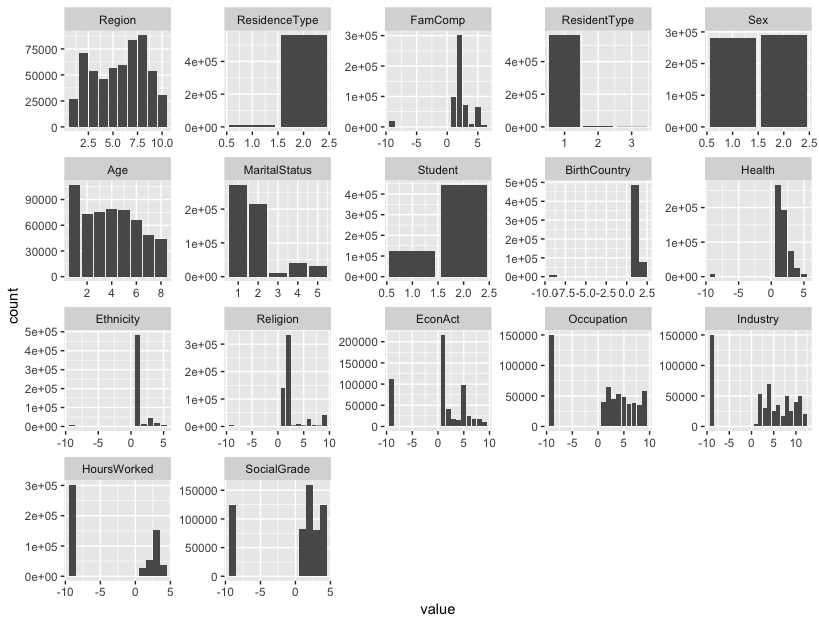
\includegraphics{images/dist_all.png}
\caption{Figure 2. Distribution of responses for variables in complete
Census Teaching File}
\end{figure}

\begin{figure}
\centering
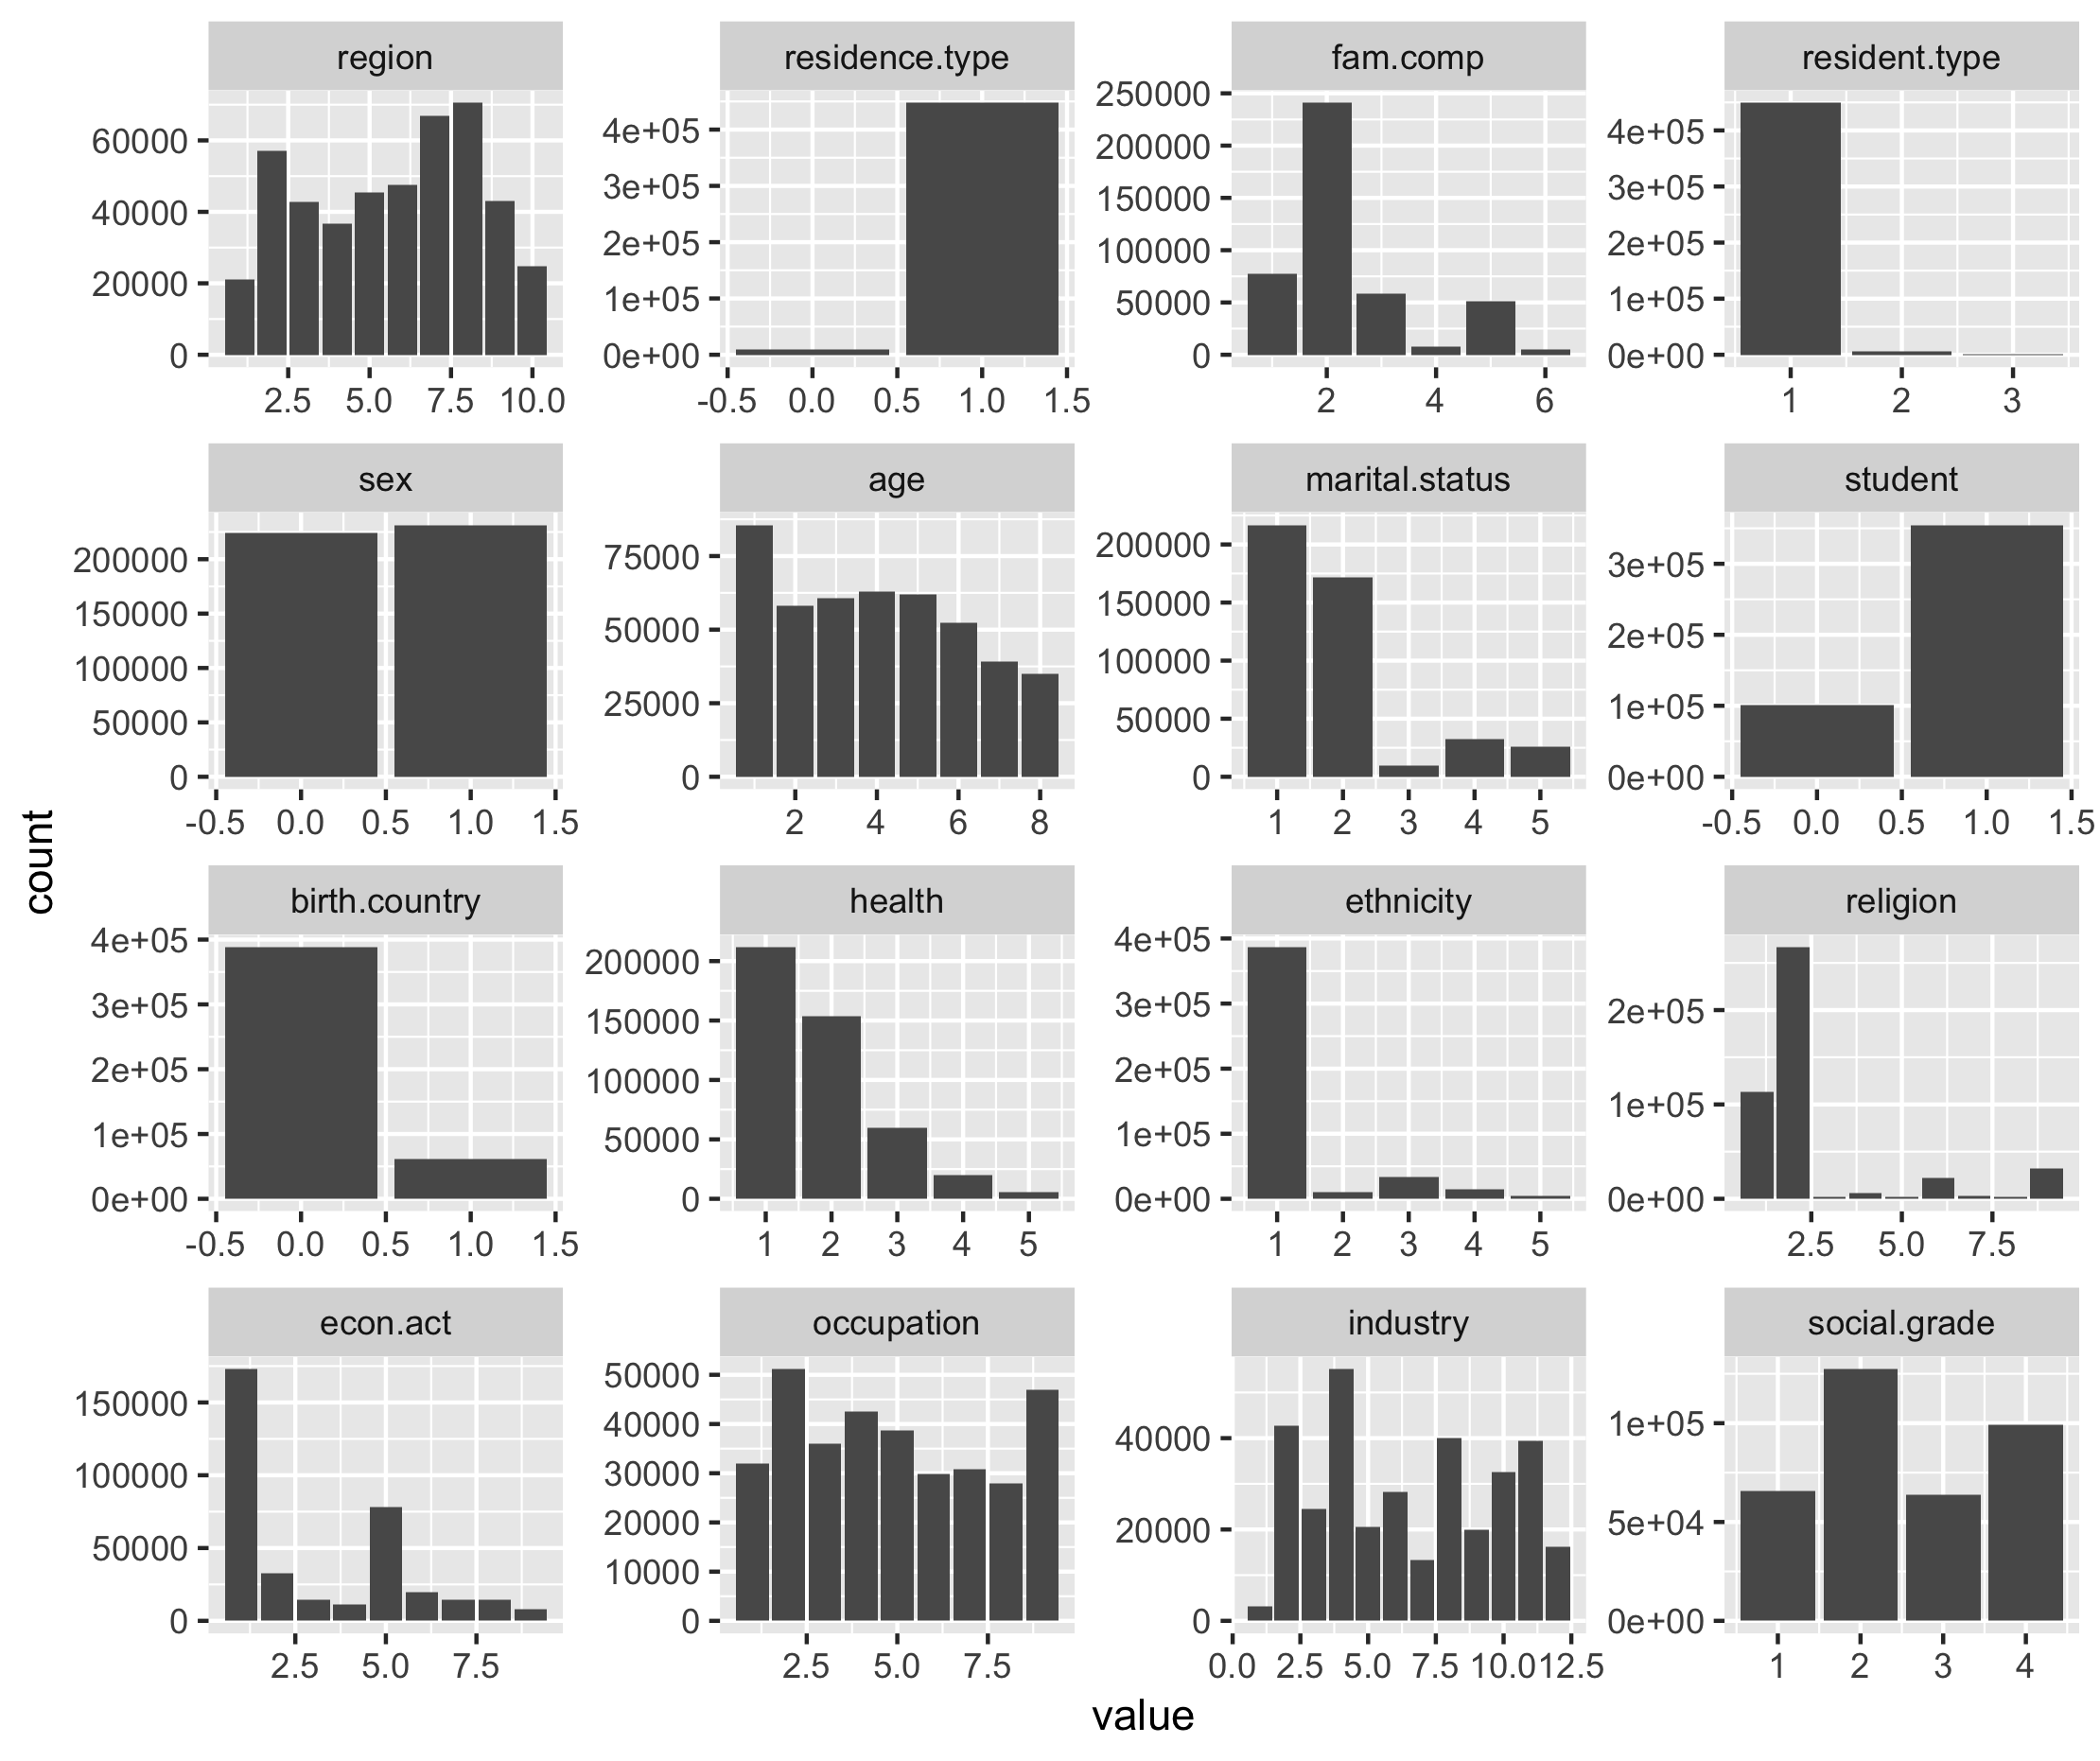
\includegraphics{images/dist_train.png}
\caption{Figure 3. Distribution of responses for variables in training
dataset}
\end{figure}

\begin{figure}
\centering
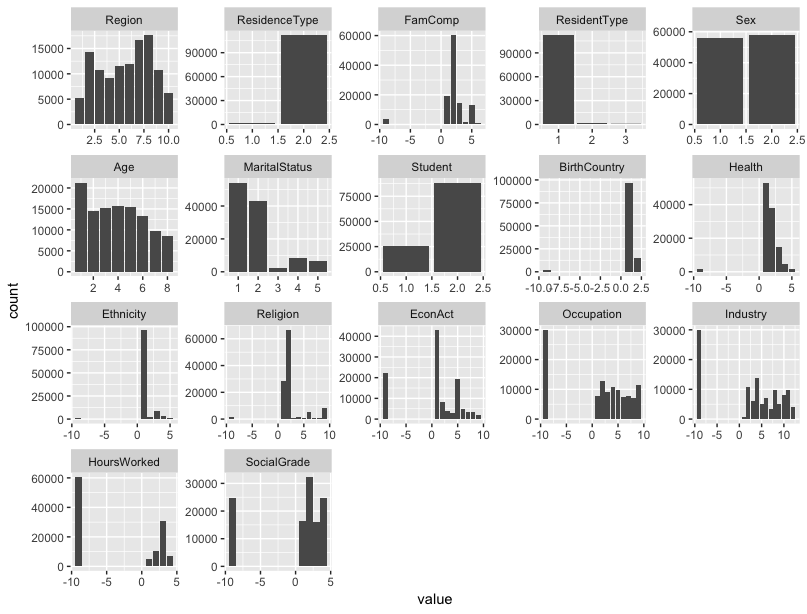
\includegraphics{images/dist_test.png}
\caption{Figure 4. Distribution of responses for variables in test
dataset}
\end{figure}

\section{Comparison of imputation
methods}\label{comparison-of-imputation-methods}

The results for the different imputation methods are presented for each
imputable variable. Performance measures were selected based on the type
of imputable variable used (i.e.~categorical or continuous). Please
refer to the links below for guidance on interpreting the performance
measures:

\begin{itemize}
\tightlist
\item
  \href{https://medium.com/human-in-a-machine-world/mae-and-rmse-which-metric-is-better-e60ac3bde13d}{Root
  mean squared error} and
  \href{https://medium.com/human-in-a-machine-world/mae-and-rmse-which-metric-is-better-e60ac3bde13d}{mean
  absolute error} (for continuous variables)\\
\item
  \href{https://www.dataschool.io/simple-guide-to-confusion-matrix-terminology/}{Confusion
  matrix} (for categorical variables)
\end{itemize}

For the categorical imputable variables, plots of the Observed vs
Predicted are provided to give an indication of which categories each
method predicted relatively well.

\subsection{Economic Activity}\label{economic-activity}

The results shows that:

\begin{itemize}
\tightlist
\item
  XGBoost predicted economic activity with greater accuracy relative to
  donor and mode imputation\\
\item
  Compared to donor based methods, the XGBoost model appeared to have
  greater sensitivity for the different classes of economic activity.
  That is, for any given class of economic activity, the model based
  approach was more likely to predict the correct response relative to
  donor based methods.
\item
  The Mixed Methods model was the least accurate imputation method for
  the multi-class variable, economic activity.
\end{itemize}

XGBoost

CANCEIS

MixedMethods

Mode

Accuracy

0.78

0.30

0.2

0.47

Kappa

0.61

0.01

0.0

NA

\begin{figure}
\centering
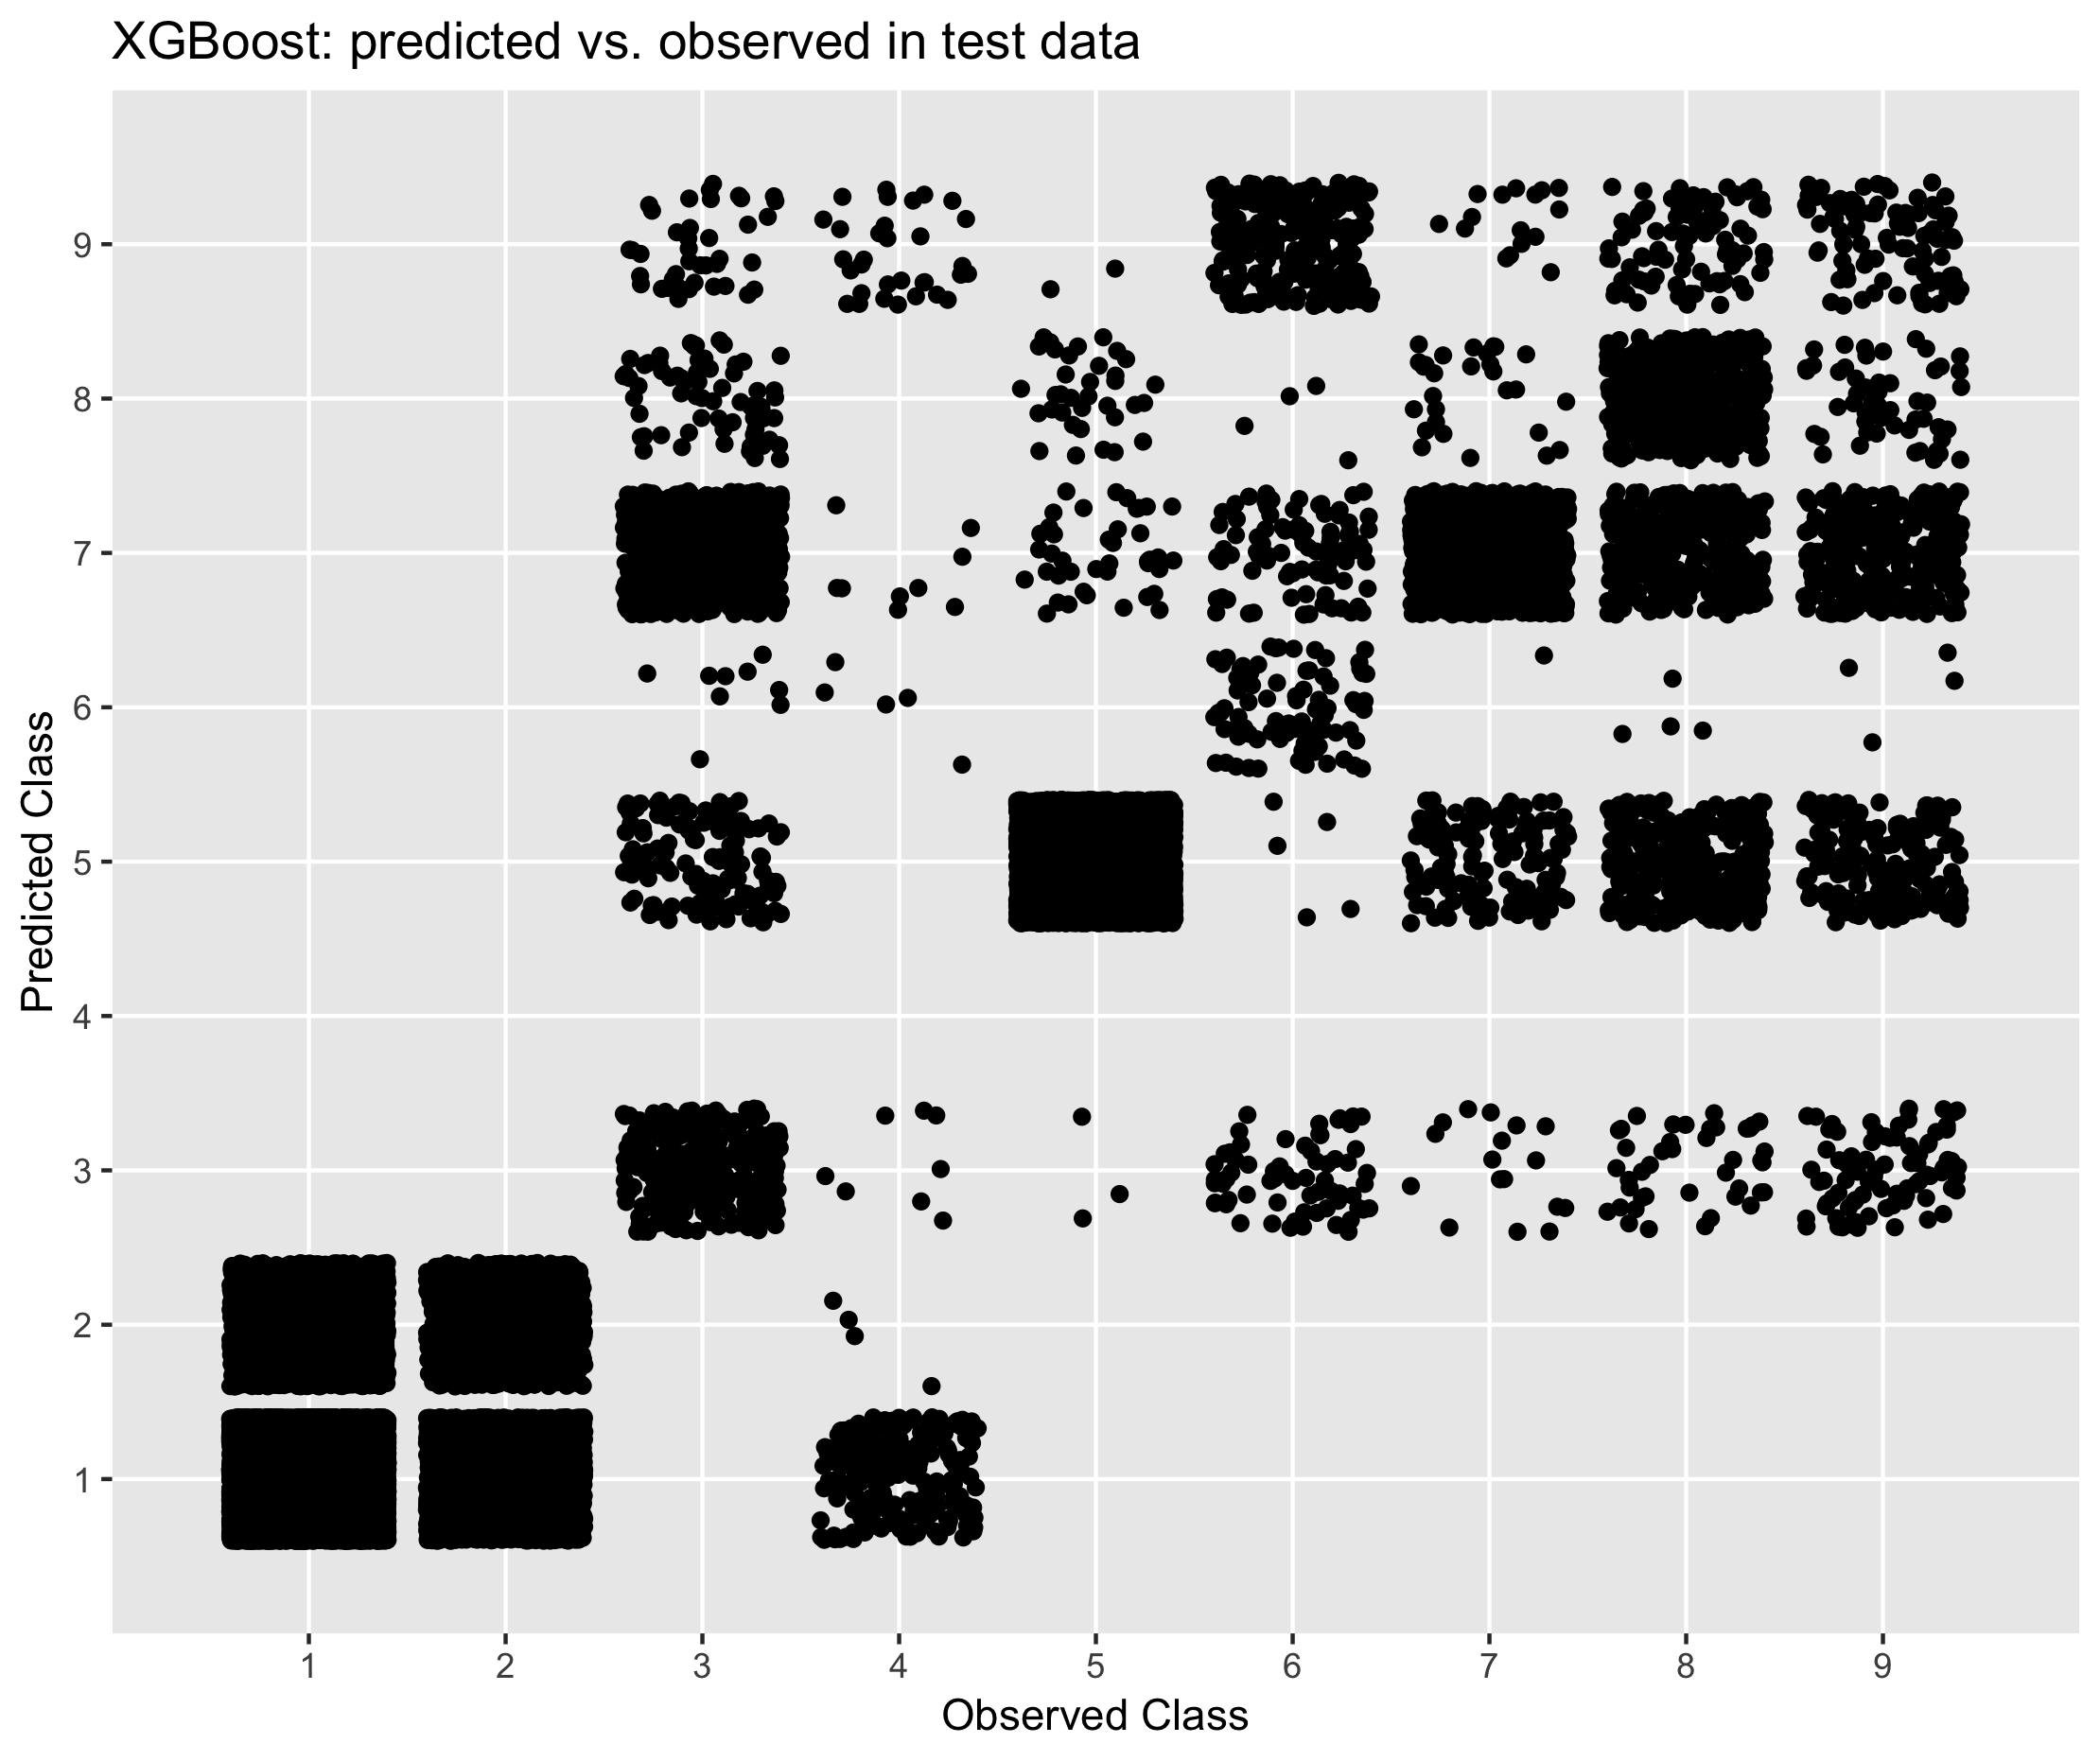
\includegraphics{images/EAXGBoostqplot.png}
\caption{Performance of XGBoost in predicting economic activity}
\end{figure}

\begin{figure}
\centering
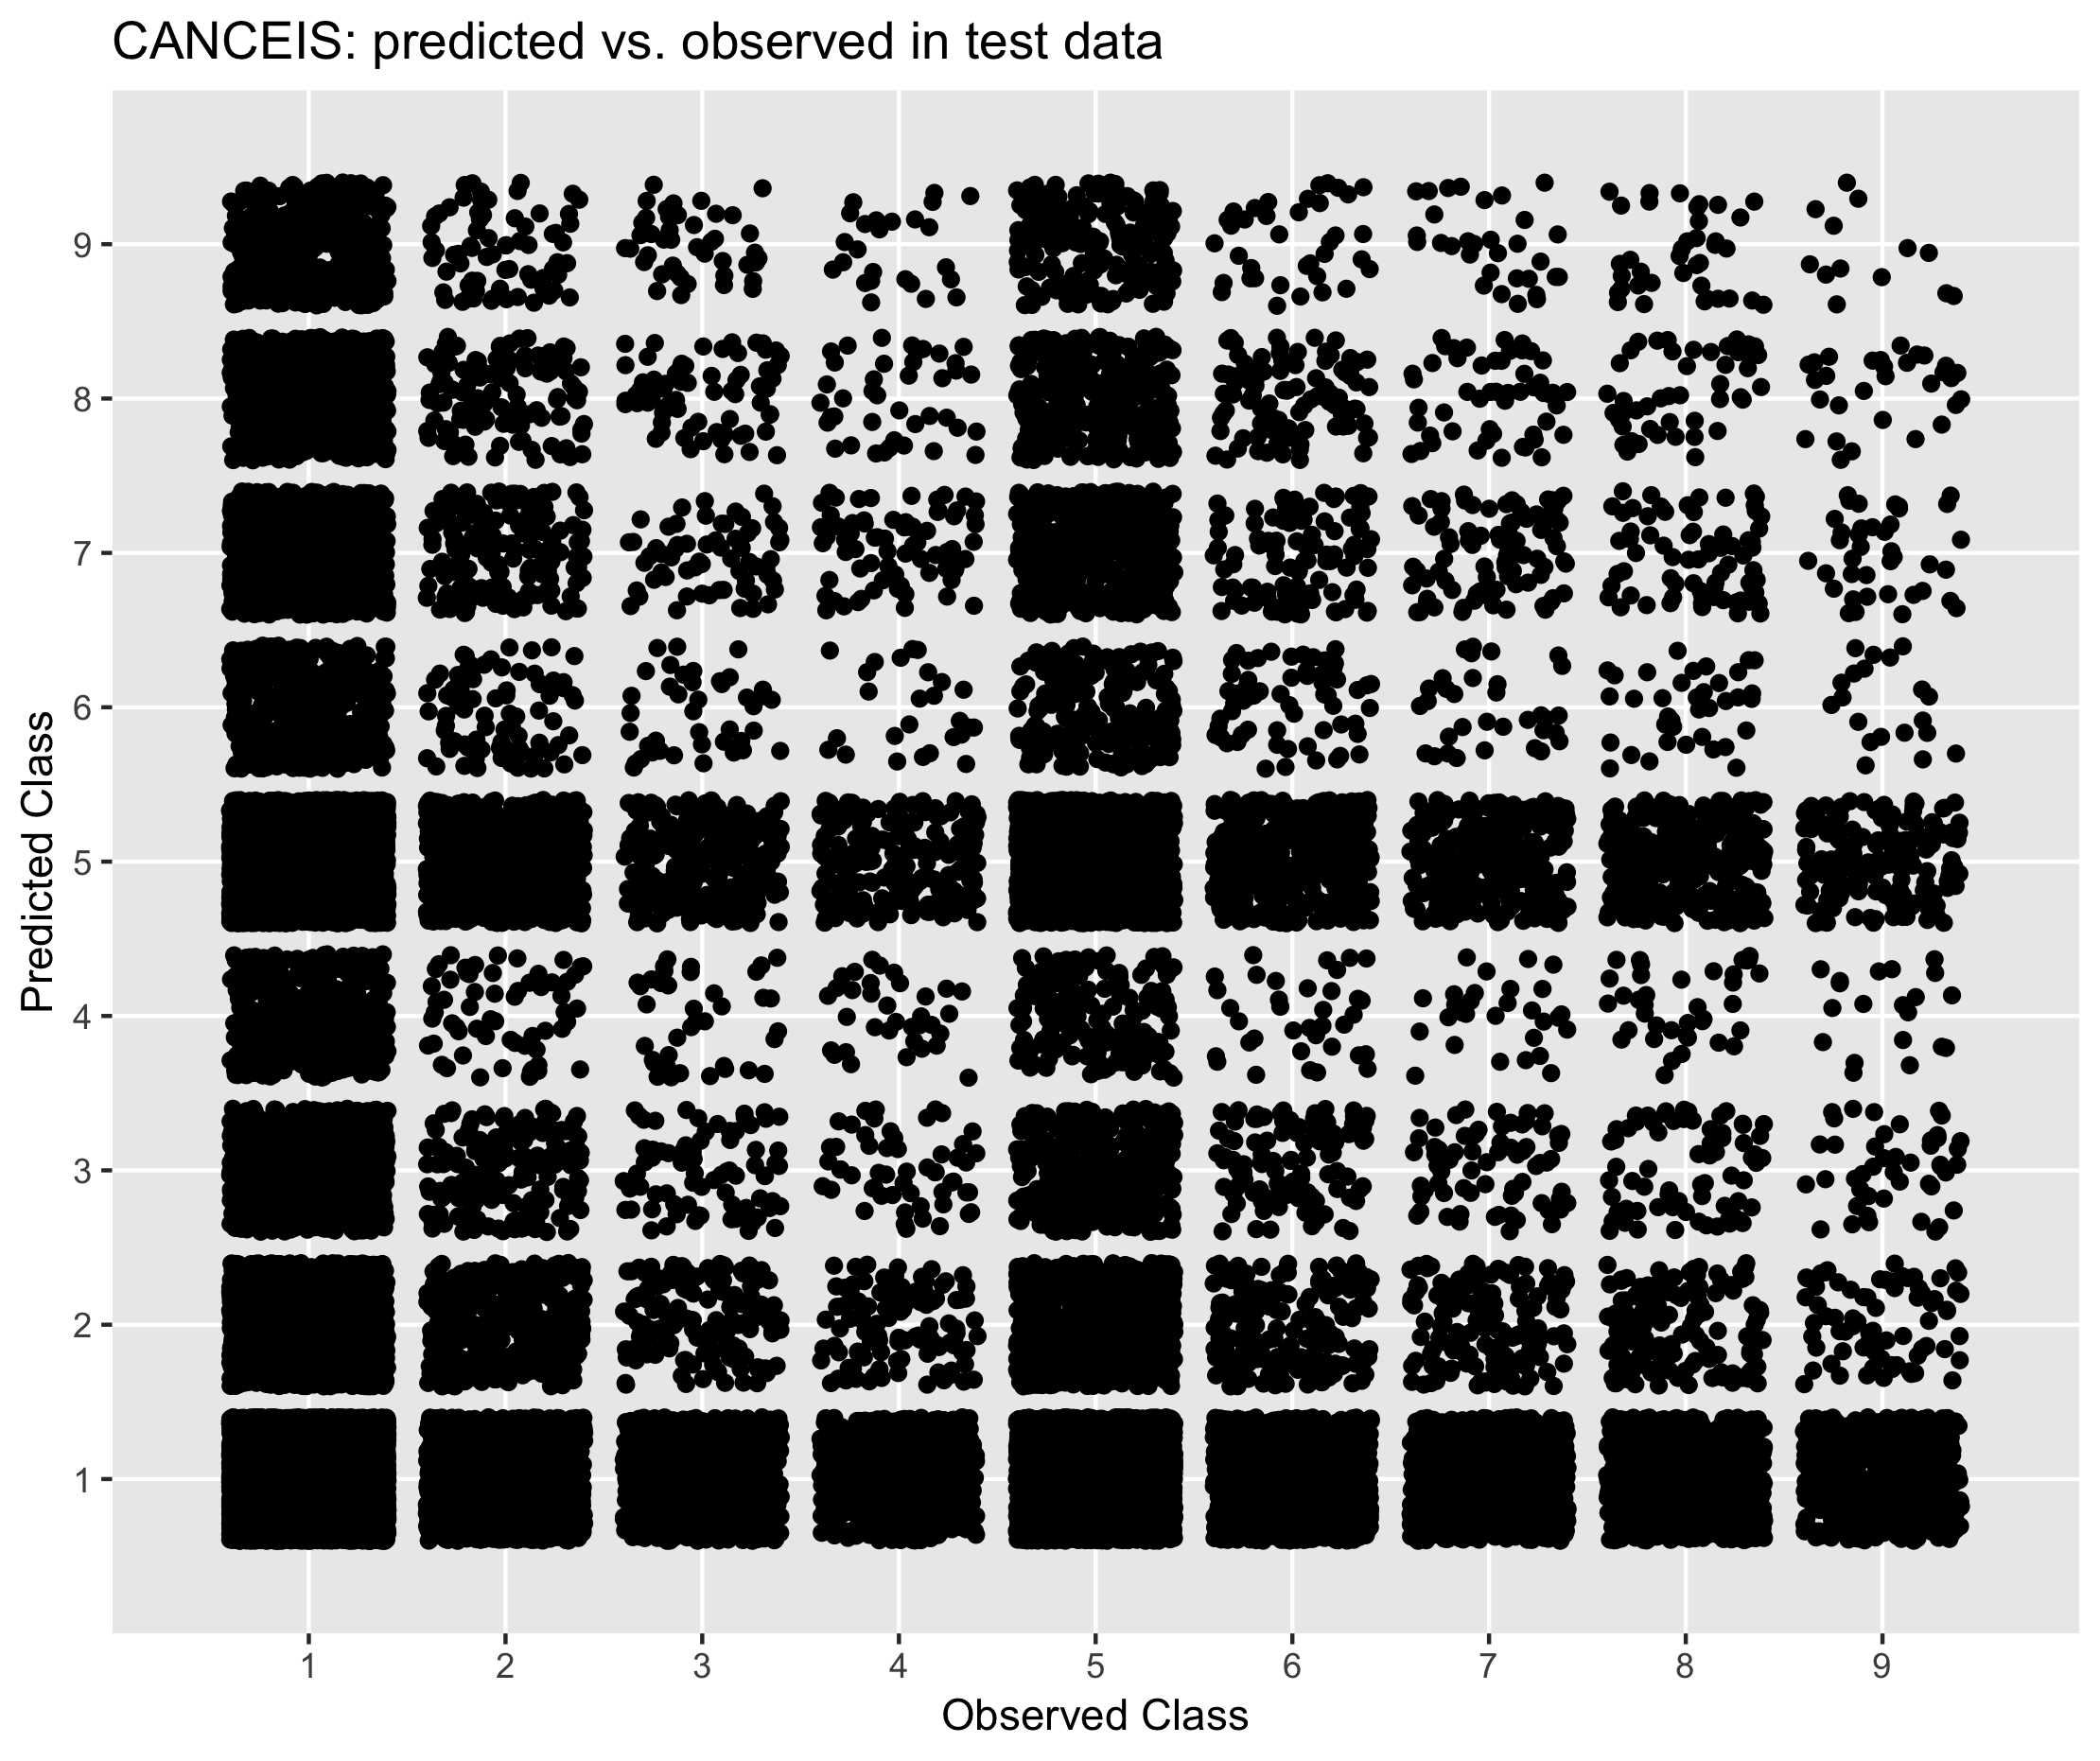
\includegraphics{images/EACANCEISqplot.png}
\caption{Performance of CANCEIS in predicting economic activity}
\end{figure}

\begin{figure}
\centering
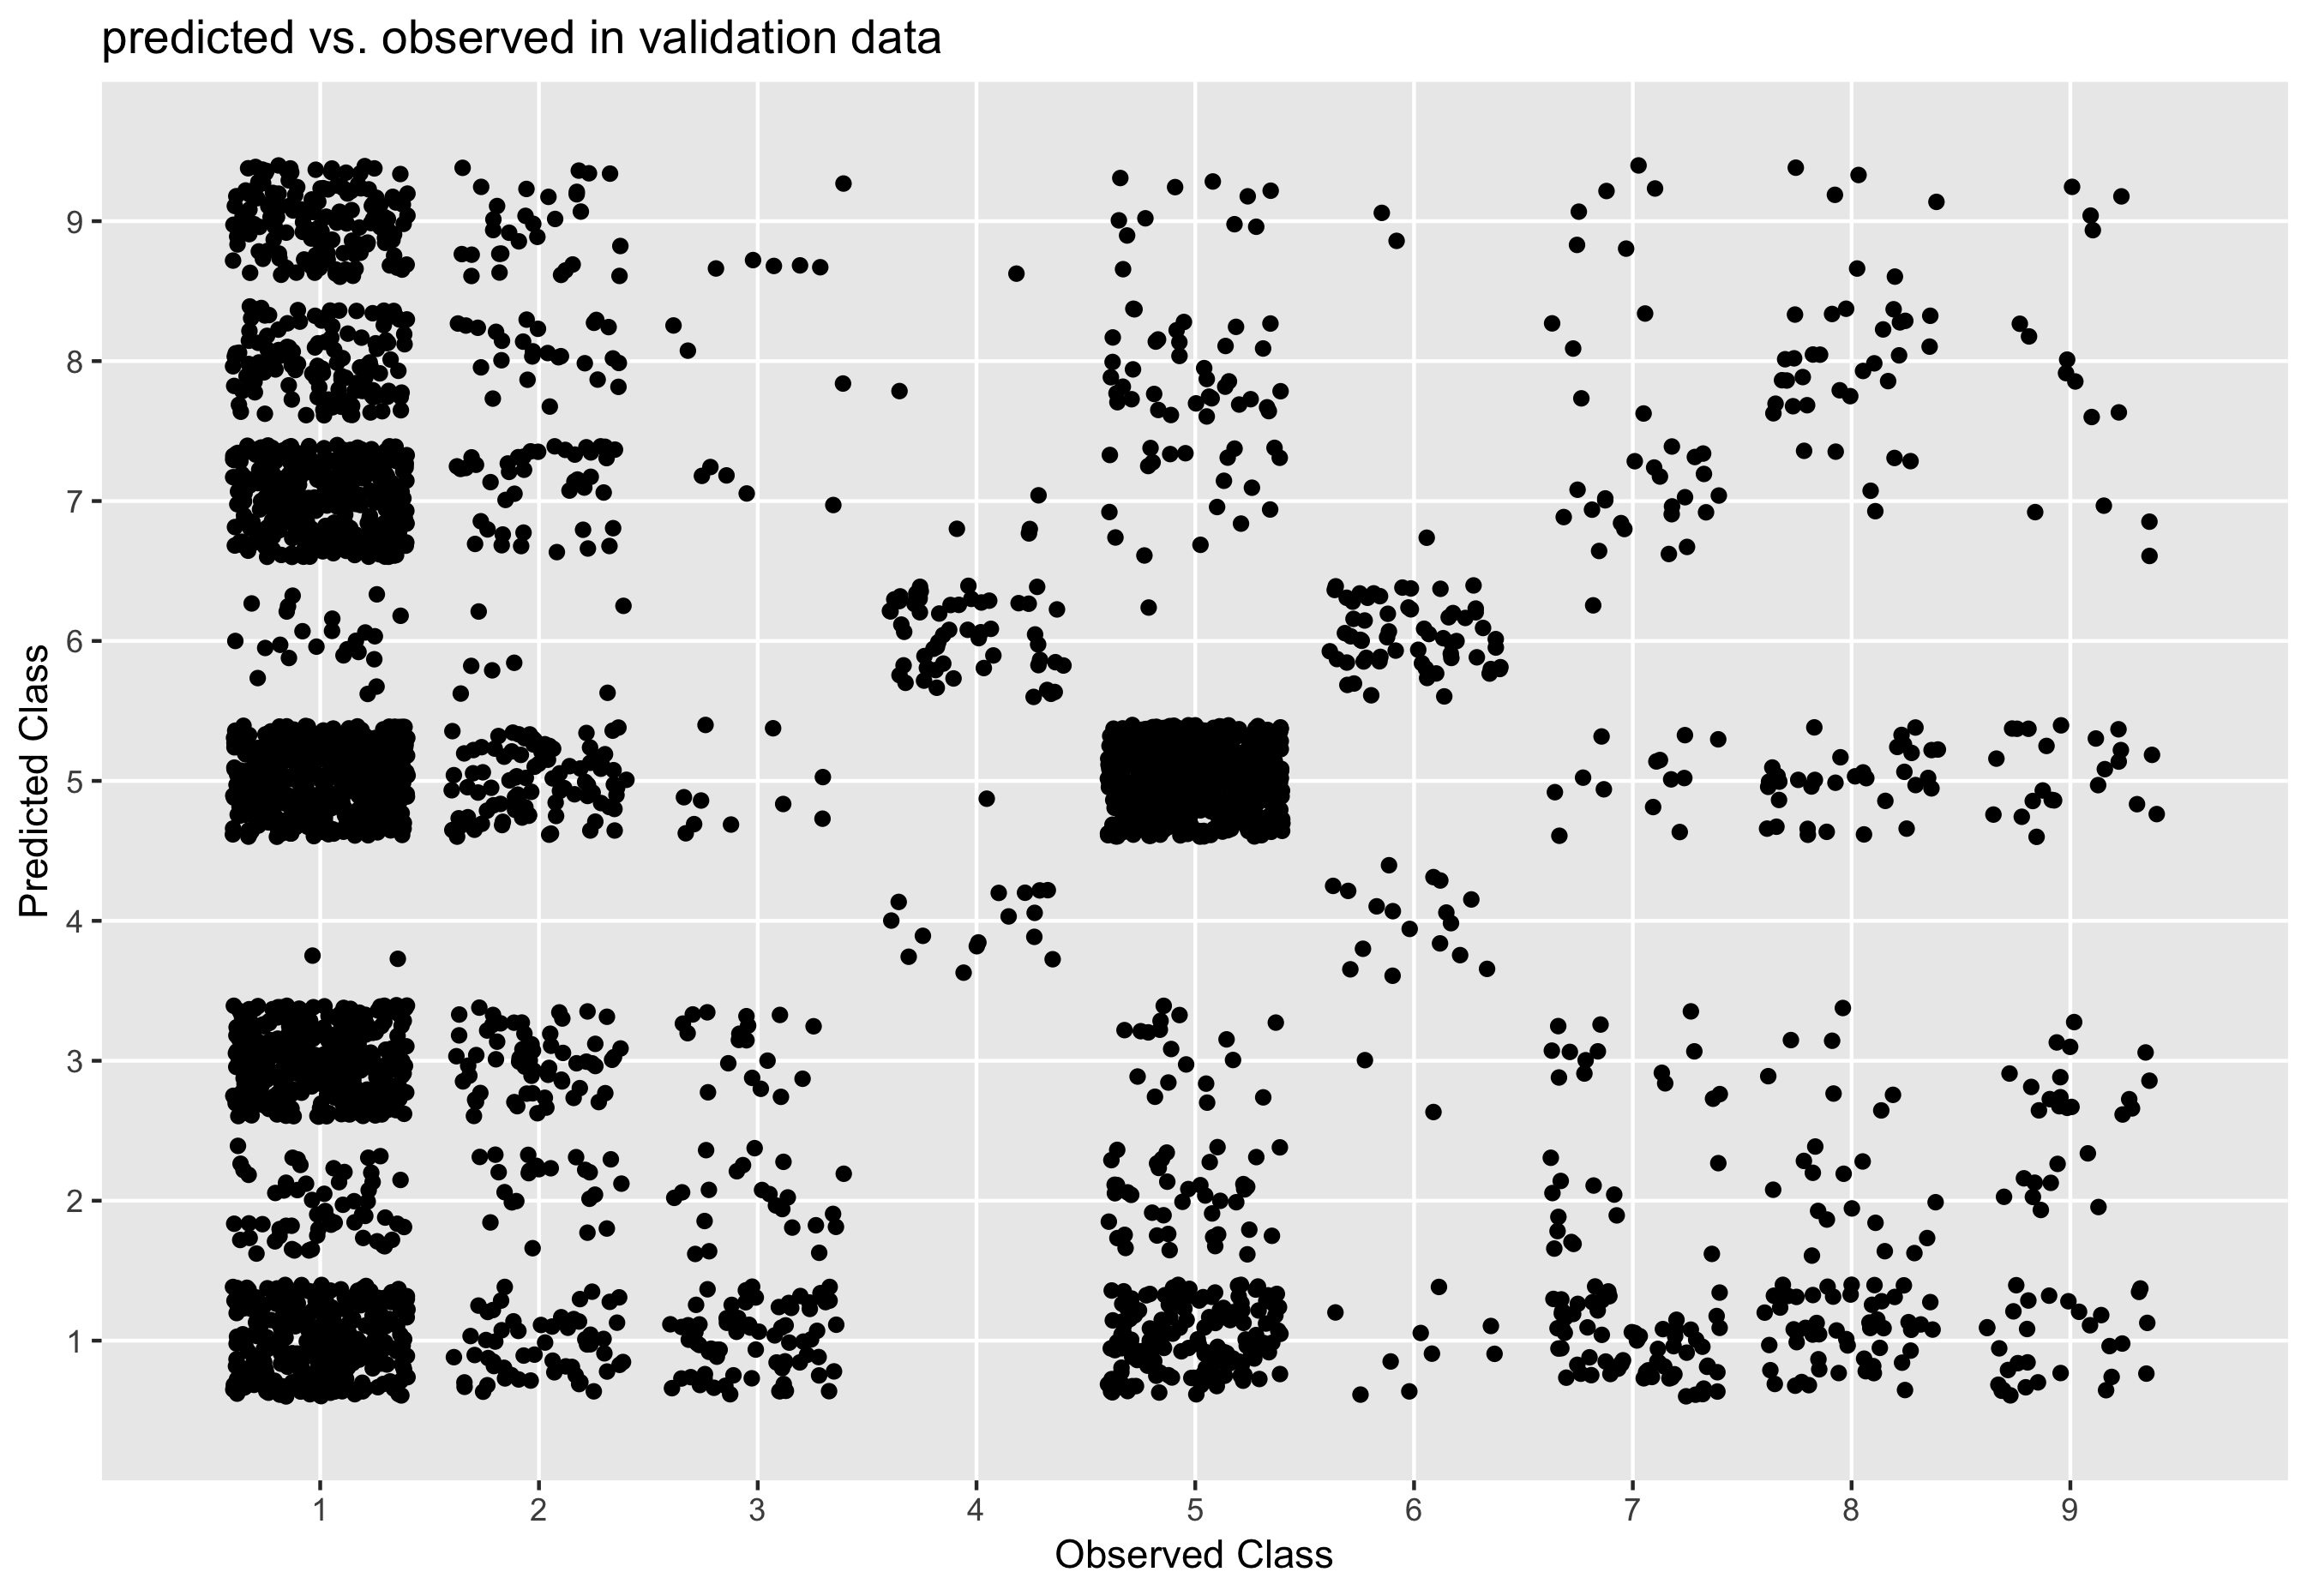
\includegraphics{images/EACANCEISXGqplot.png}
\caption{Performance of Mixed Methods approach in predicting economic
activity}
\end{figure}

\subsection{Hours worked}\label{hours-worked}

The results shows that:

\begin{itemize}
\tightlist
\item
  XGBoost predicted hours worked with greater accuracy relative to donor
  and mode imputation\\
\item
  Median imputation and the Mixed Methods approach had a similar level
  of accuracy\\
\item
  Donor based imputation had the lowest level of accuracy
\end{itemize}

XGBoost

CANCEIS

MixedMethods

Median

MAE

9.71

14.64

14.62

10.51

RMSE

12.31

18.53

18.52

13.5

\subsection{Social Grade}\label{social-grade}

The results shows that:

\begin{itemize}
\tightlist
\item
  All three approaches performed with similar degree of accuracy, whilst
  out-performing mode imputation\\
\item
  Compared to donor based methods, the XGBoost model appeared to have
  greater sensitivity for the different classes of social grade. That
  is, for any given class of social grade, the model based approach was
  more likely to predict the correct response relative to donor based
  methods.
\end{itemize}

XGBoost

CANCEIS

MixedMethods

Mode

Accuracy

0.62

0.28

0.28

0.36

Kappa

0.49

0.01

0.01

NA

\begin{figure}
\centering
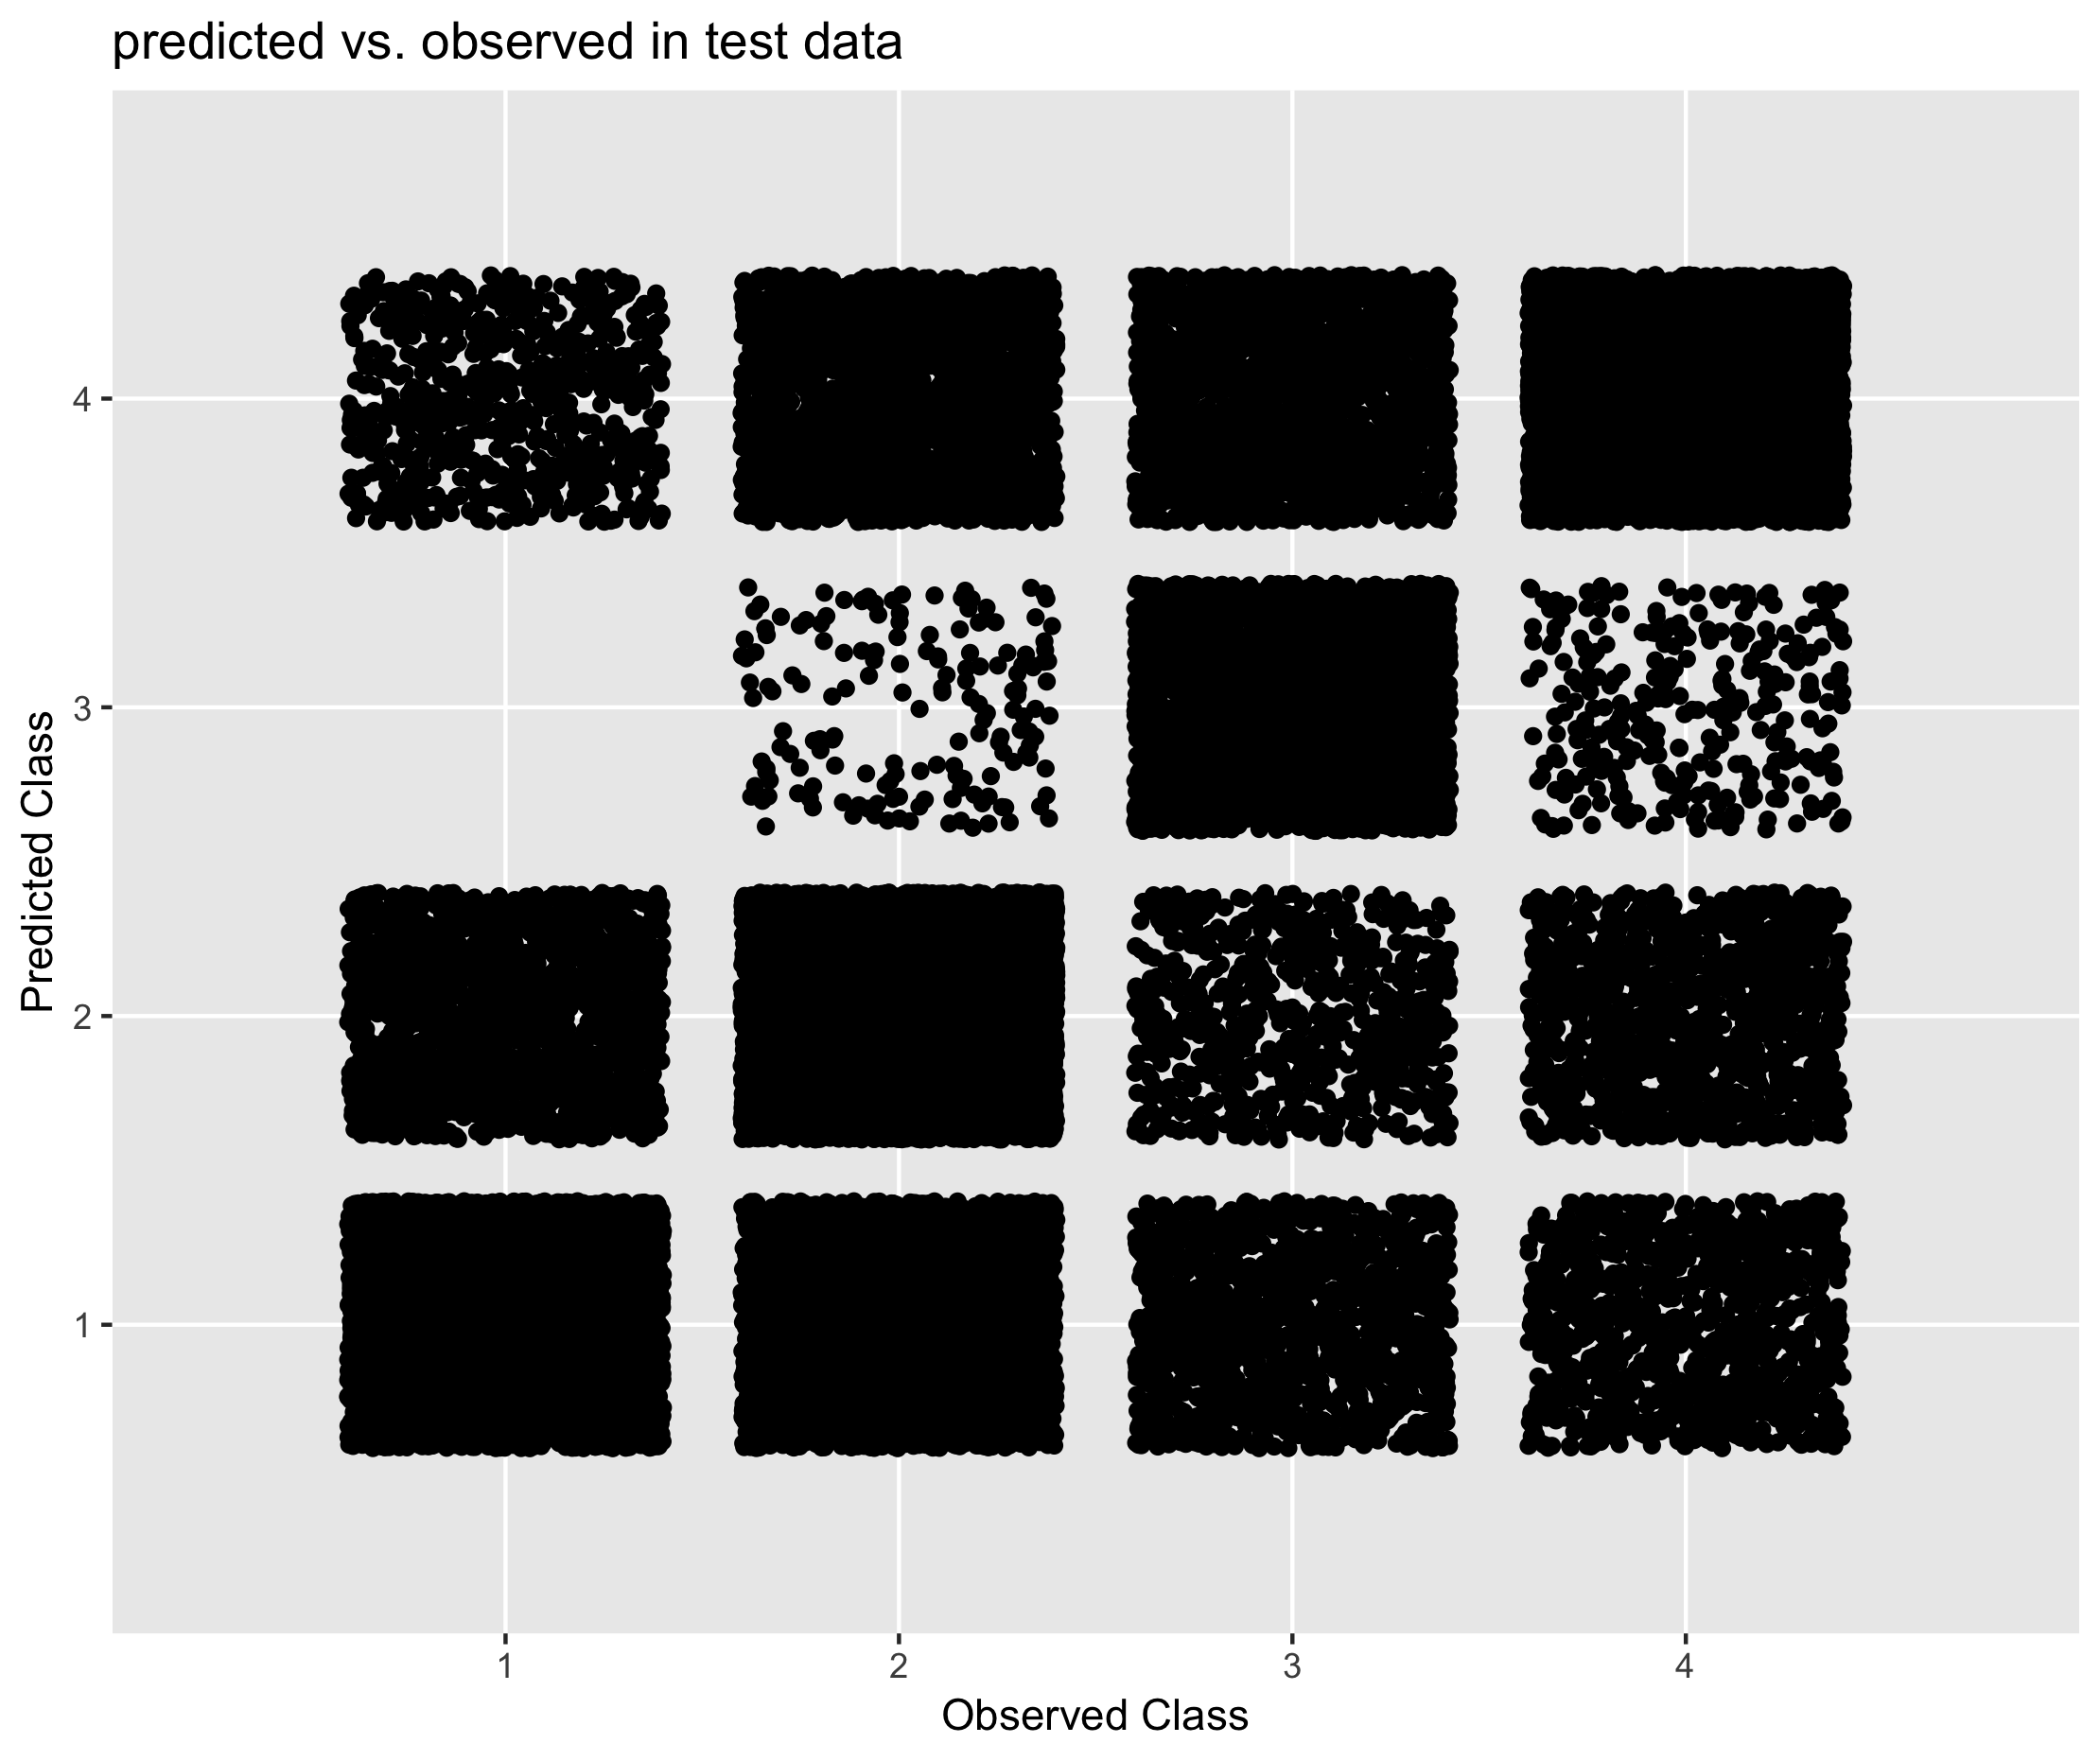
\includegraphics{images/SGXGBoostqplot.png}
\caption{Performance of XGBoost in predicting social grade}
\end{figure}

\begin{figure}
\centering
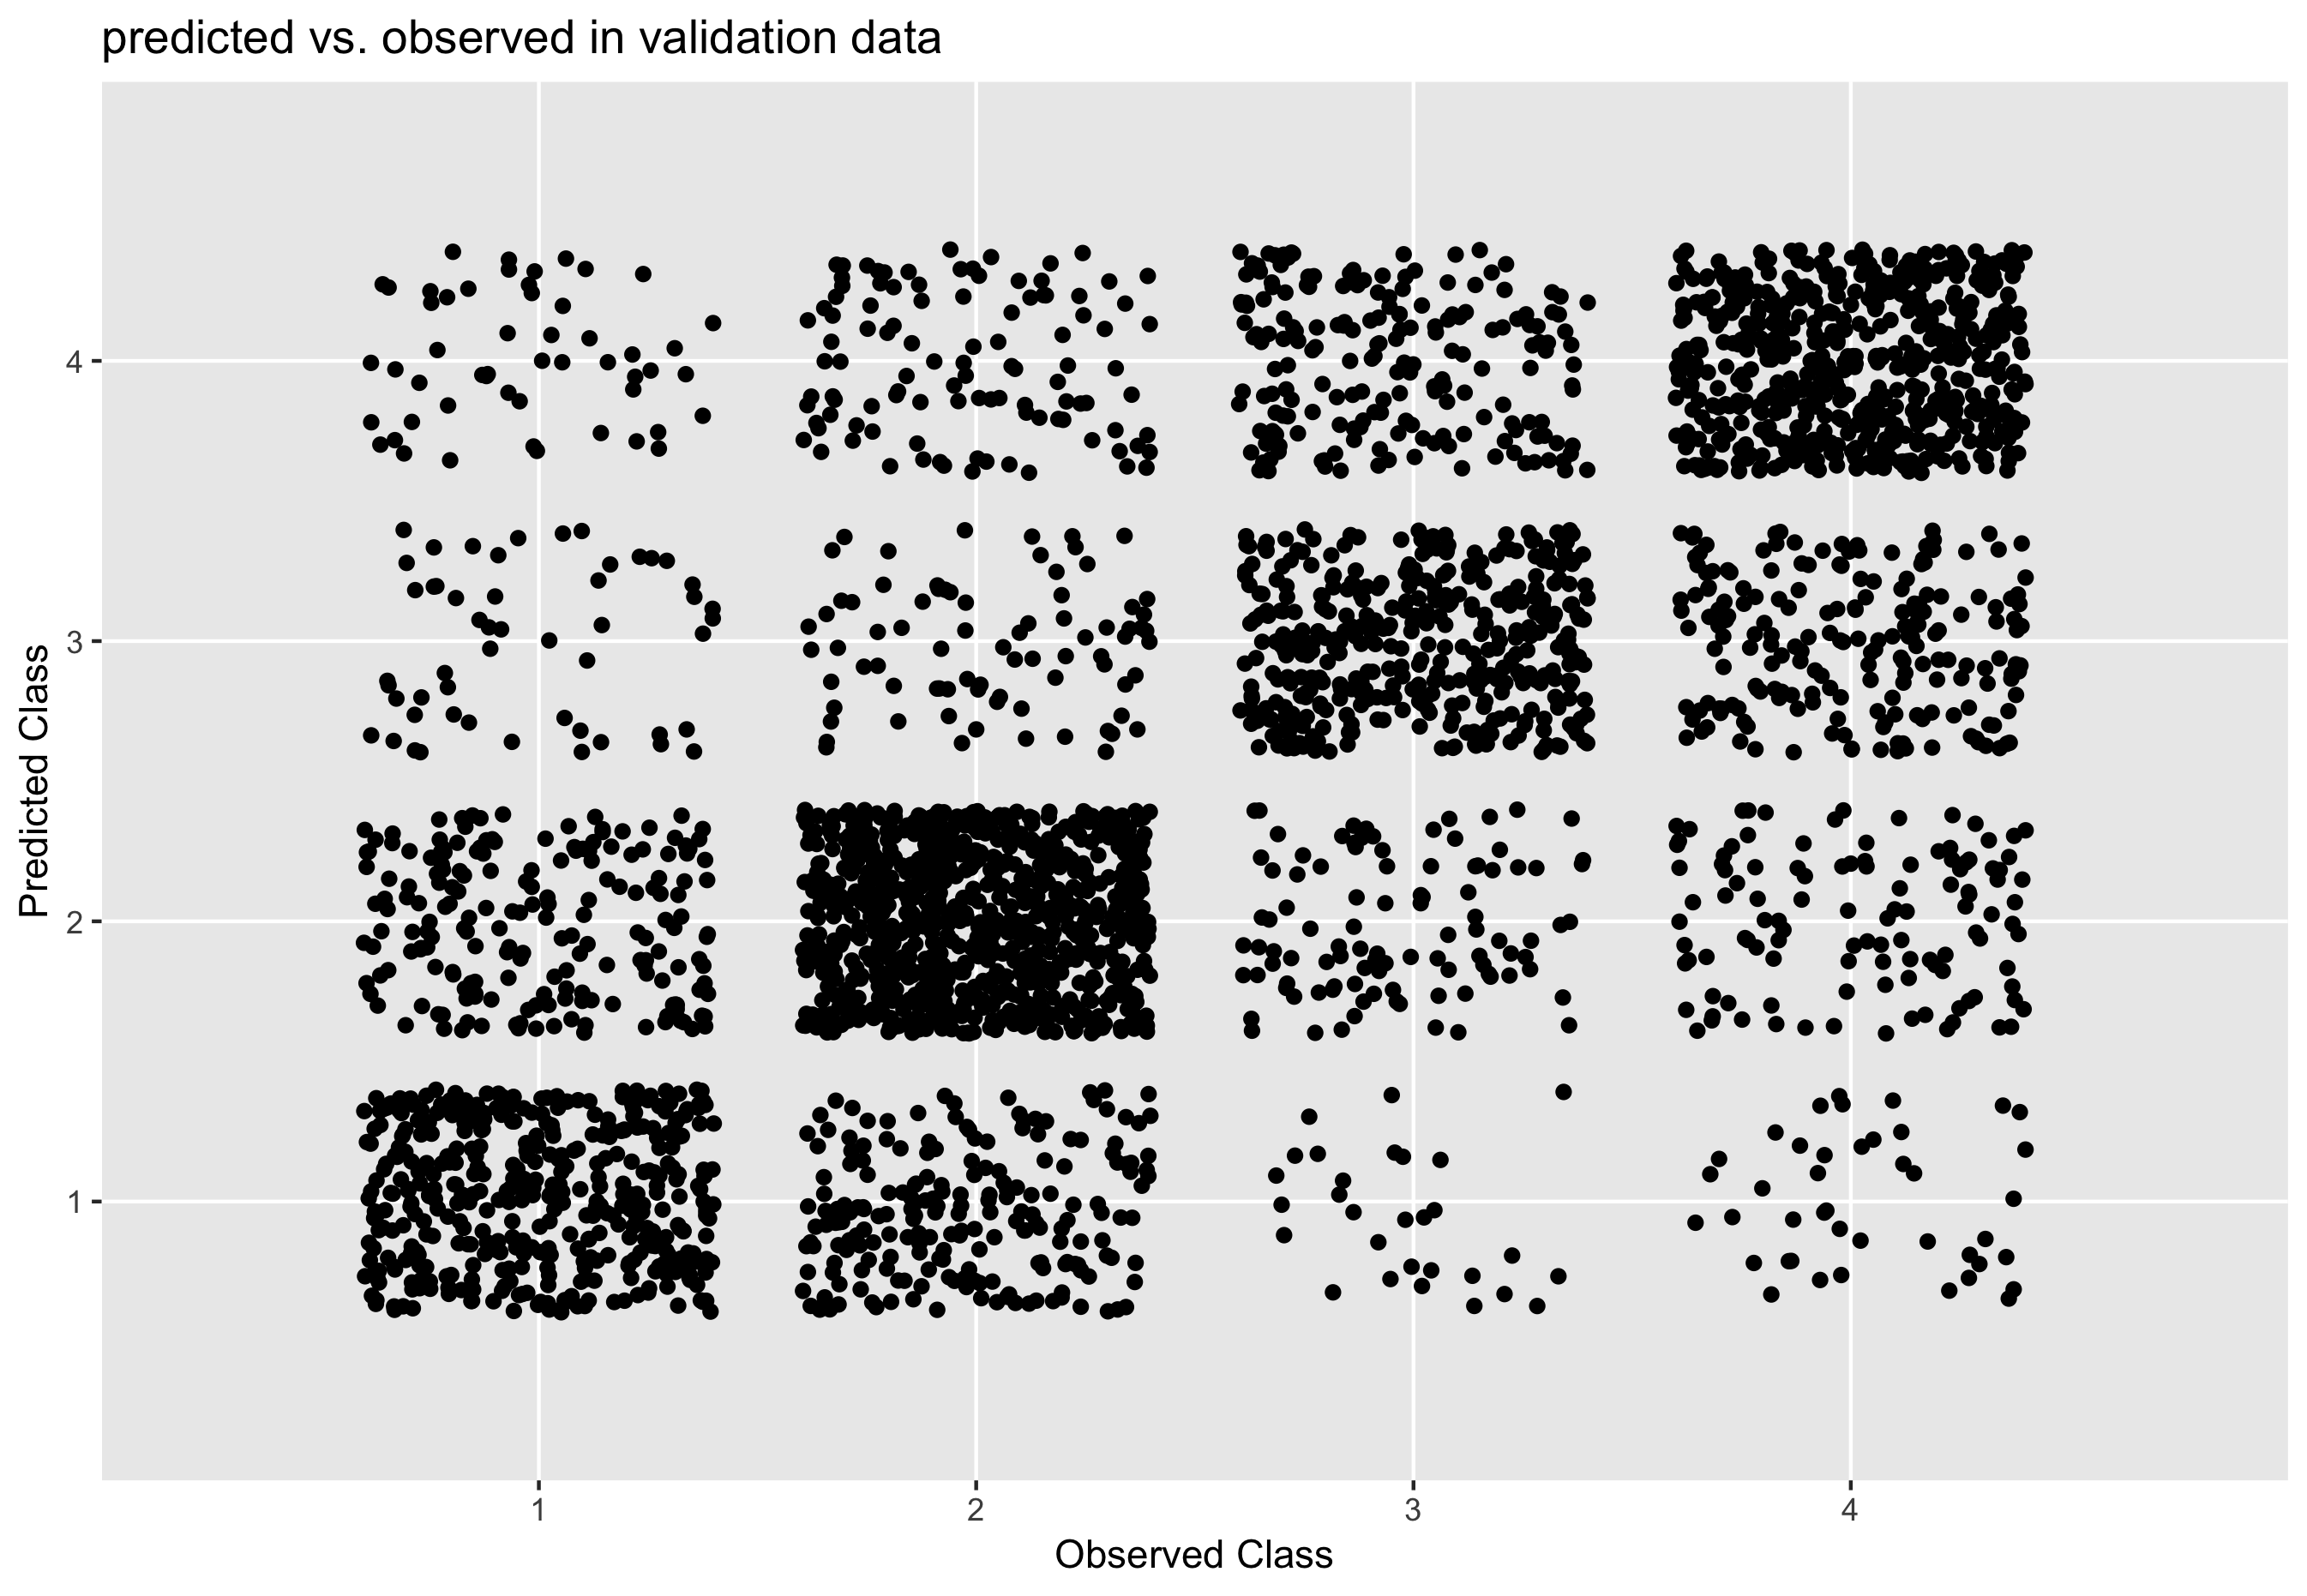
\includegraphics{images/SGCANCEISqplot.png}
\caption{Performance of CANCEIS in predicting social grade}
\end{figure}

\begin{figure}
\centering
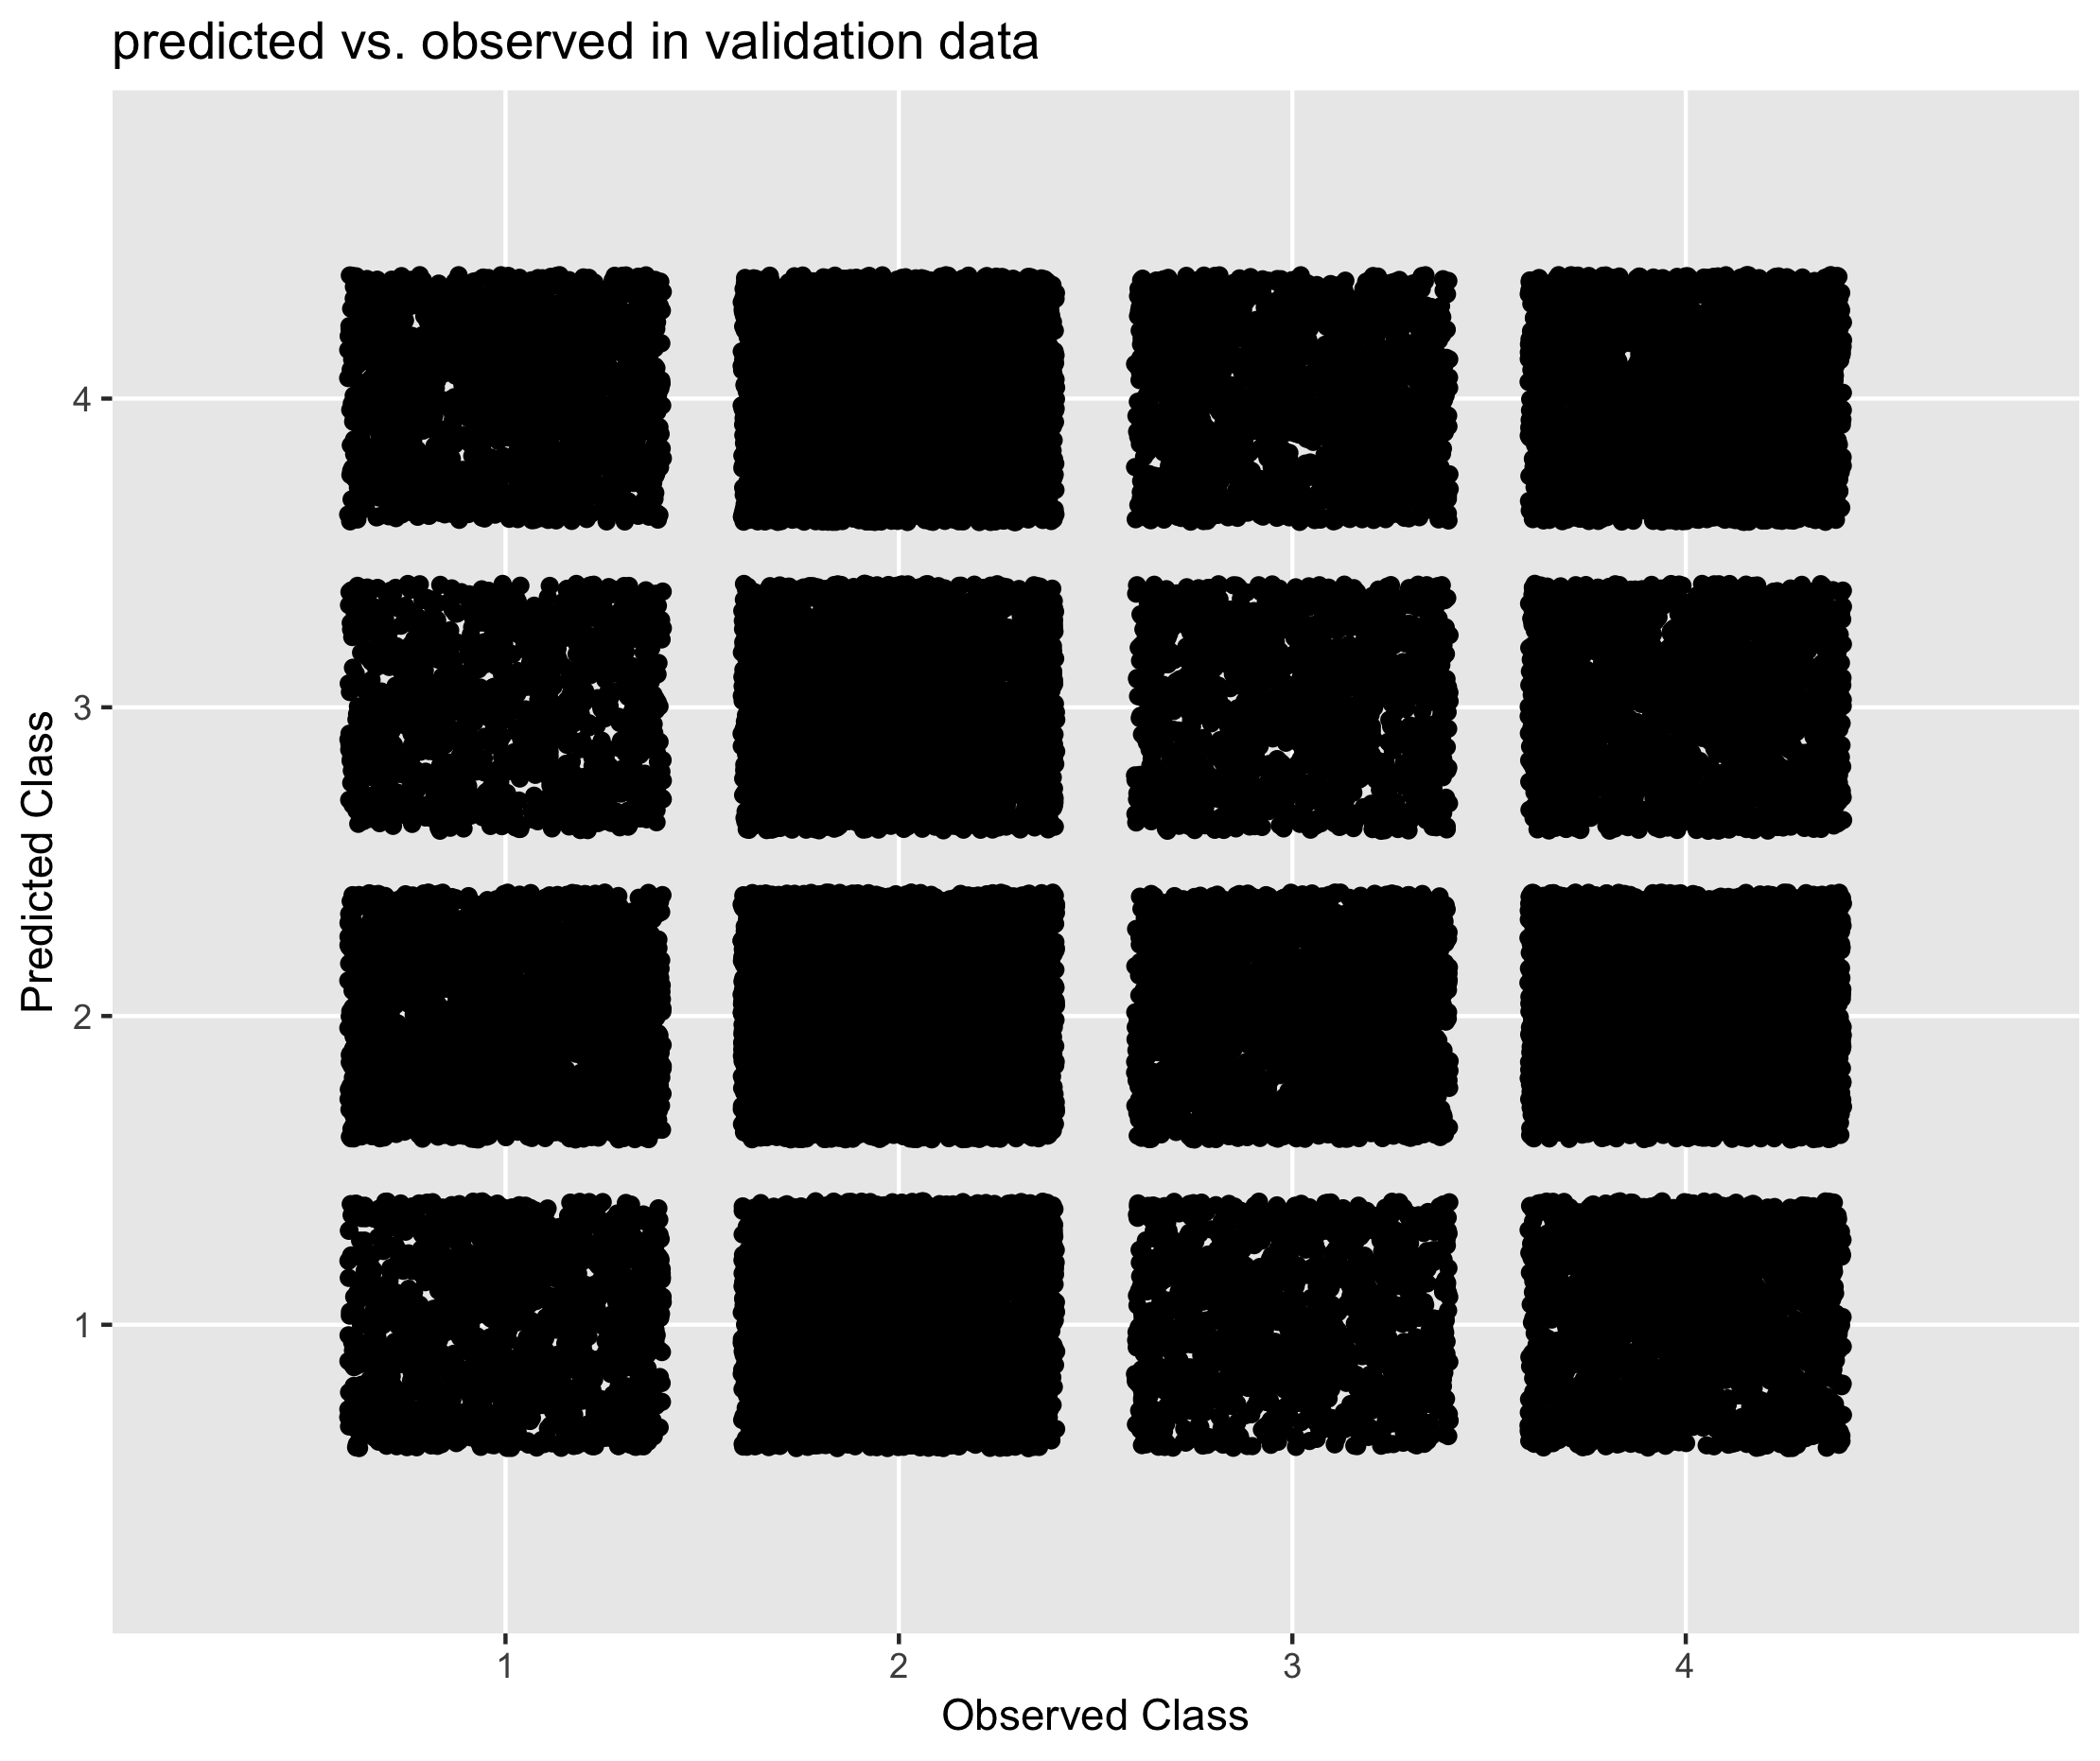
\includegraphics{images/SGCANCEISXGqplot.png}
\caption{Performance of Mixed Methods approach in predicting social
grade}
\end{figure}

\subsection{Student}\label{student}

The results shows that:

\begin{itemize}
\tightlist
\item
  All three approaches performed with similar degree of accuracy, whilst
  out-performing mode imputation\\
\item
  Compared to donor based methods, the XGBoost model appeared to have
  greater sensitivity for the different classes of student status. That
  is, for both students and non-students, the model based approach was
  more likely to predict the correct response relative to donor based
  methods.
\end{itemize}

XGBoost

CANCEIS

MixedMethods

Mode

Accuracy

0.9747038

0.6984867

0.6819554

0.7763281

Kappa

0.9192150

-0.0015287

-0.0000217

NA

\begin{figure}
\centering
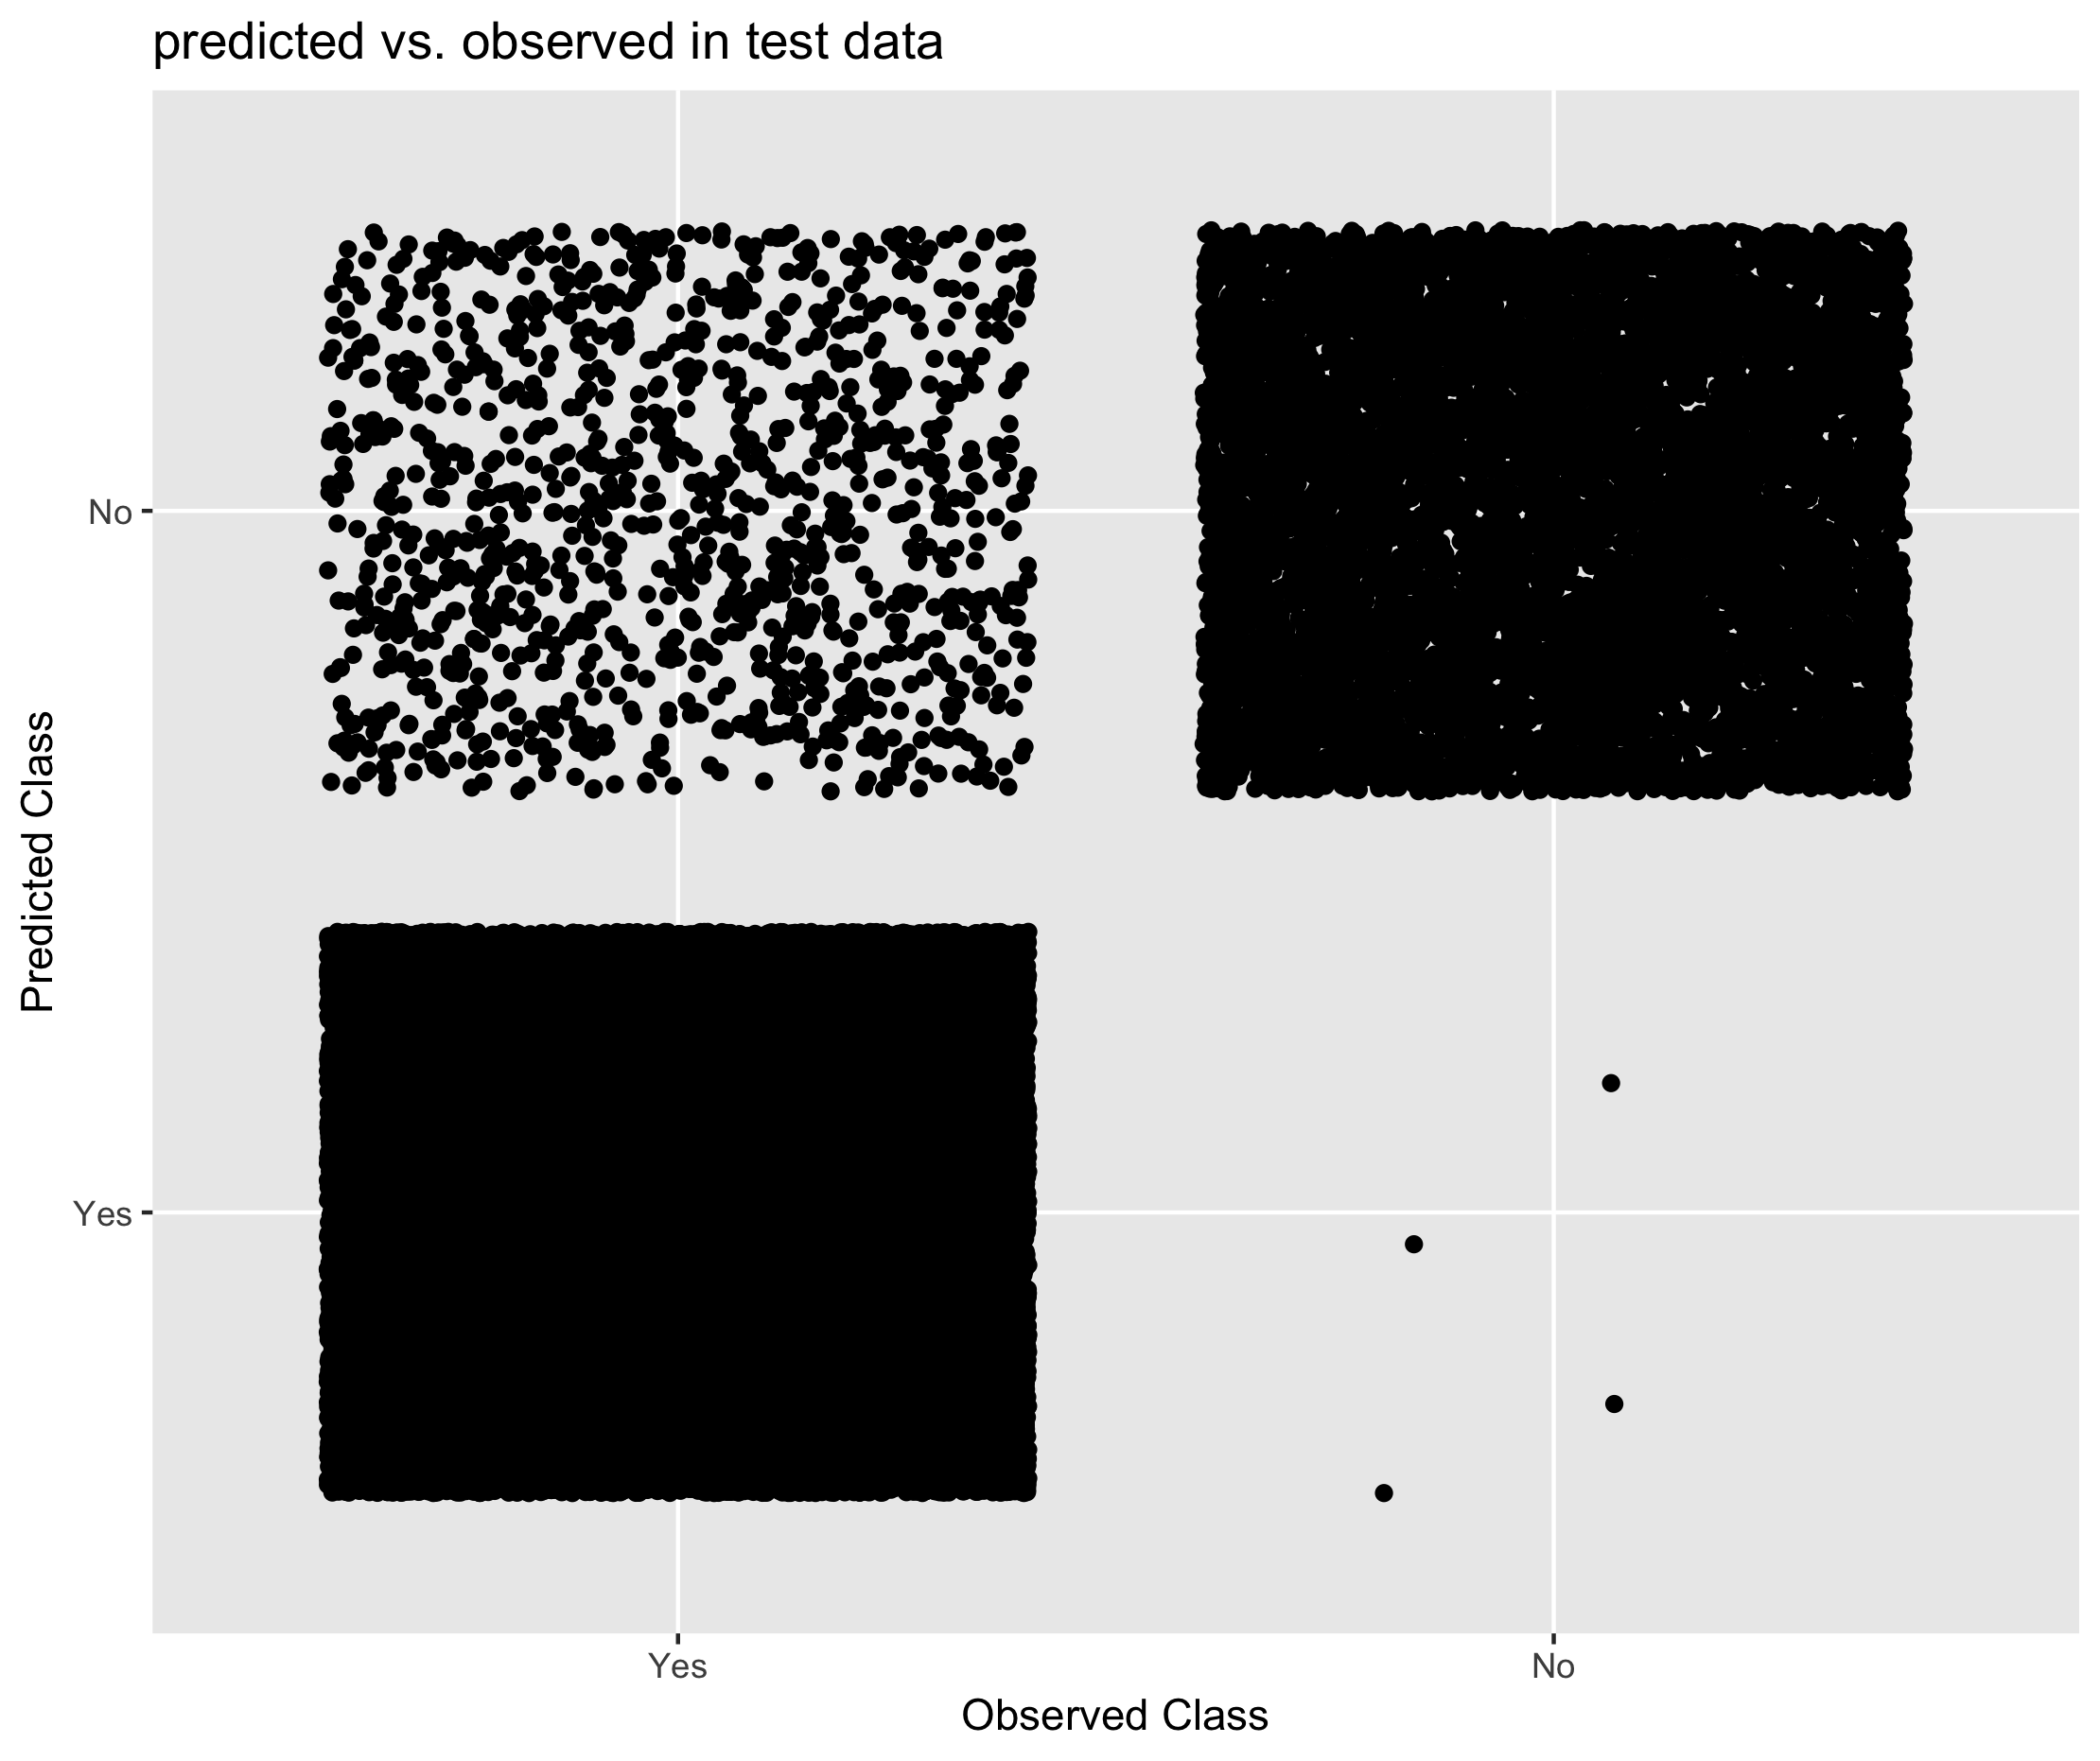
\includegraphics{images/STXGBoostqplot.png}
\caption{Performance of XGBoost in predicting student status}
\end{figure}

\begin{figure}
\centering
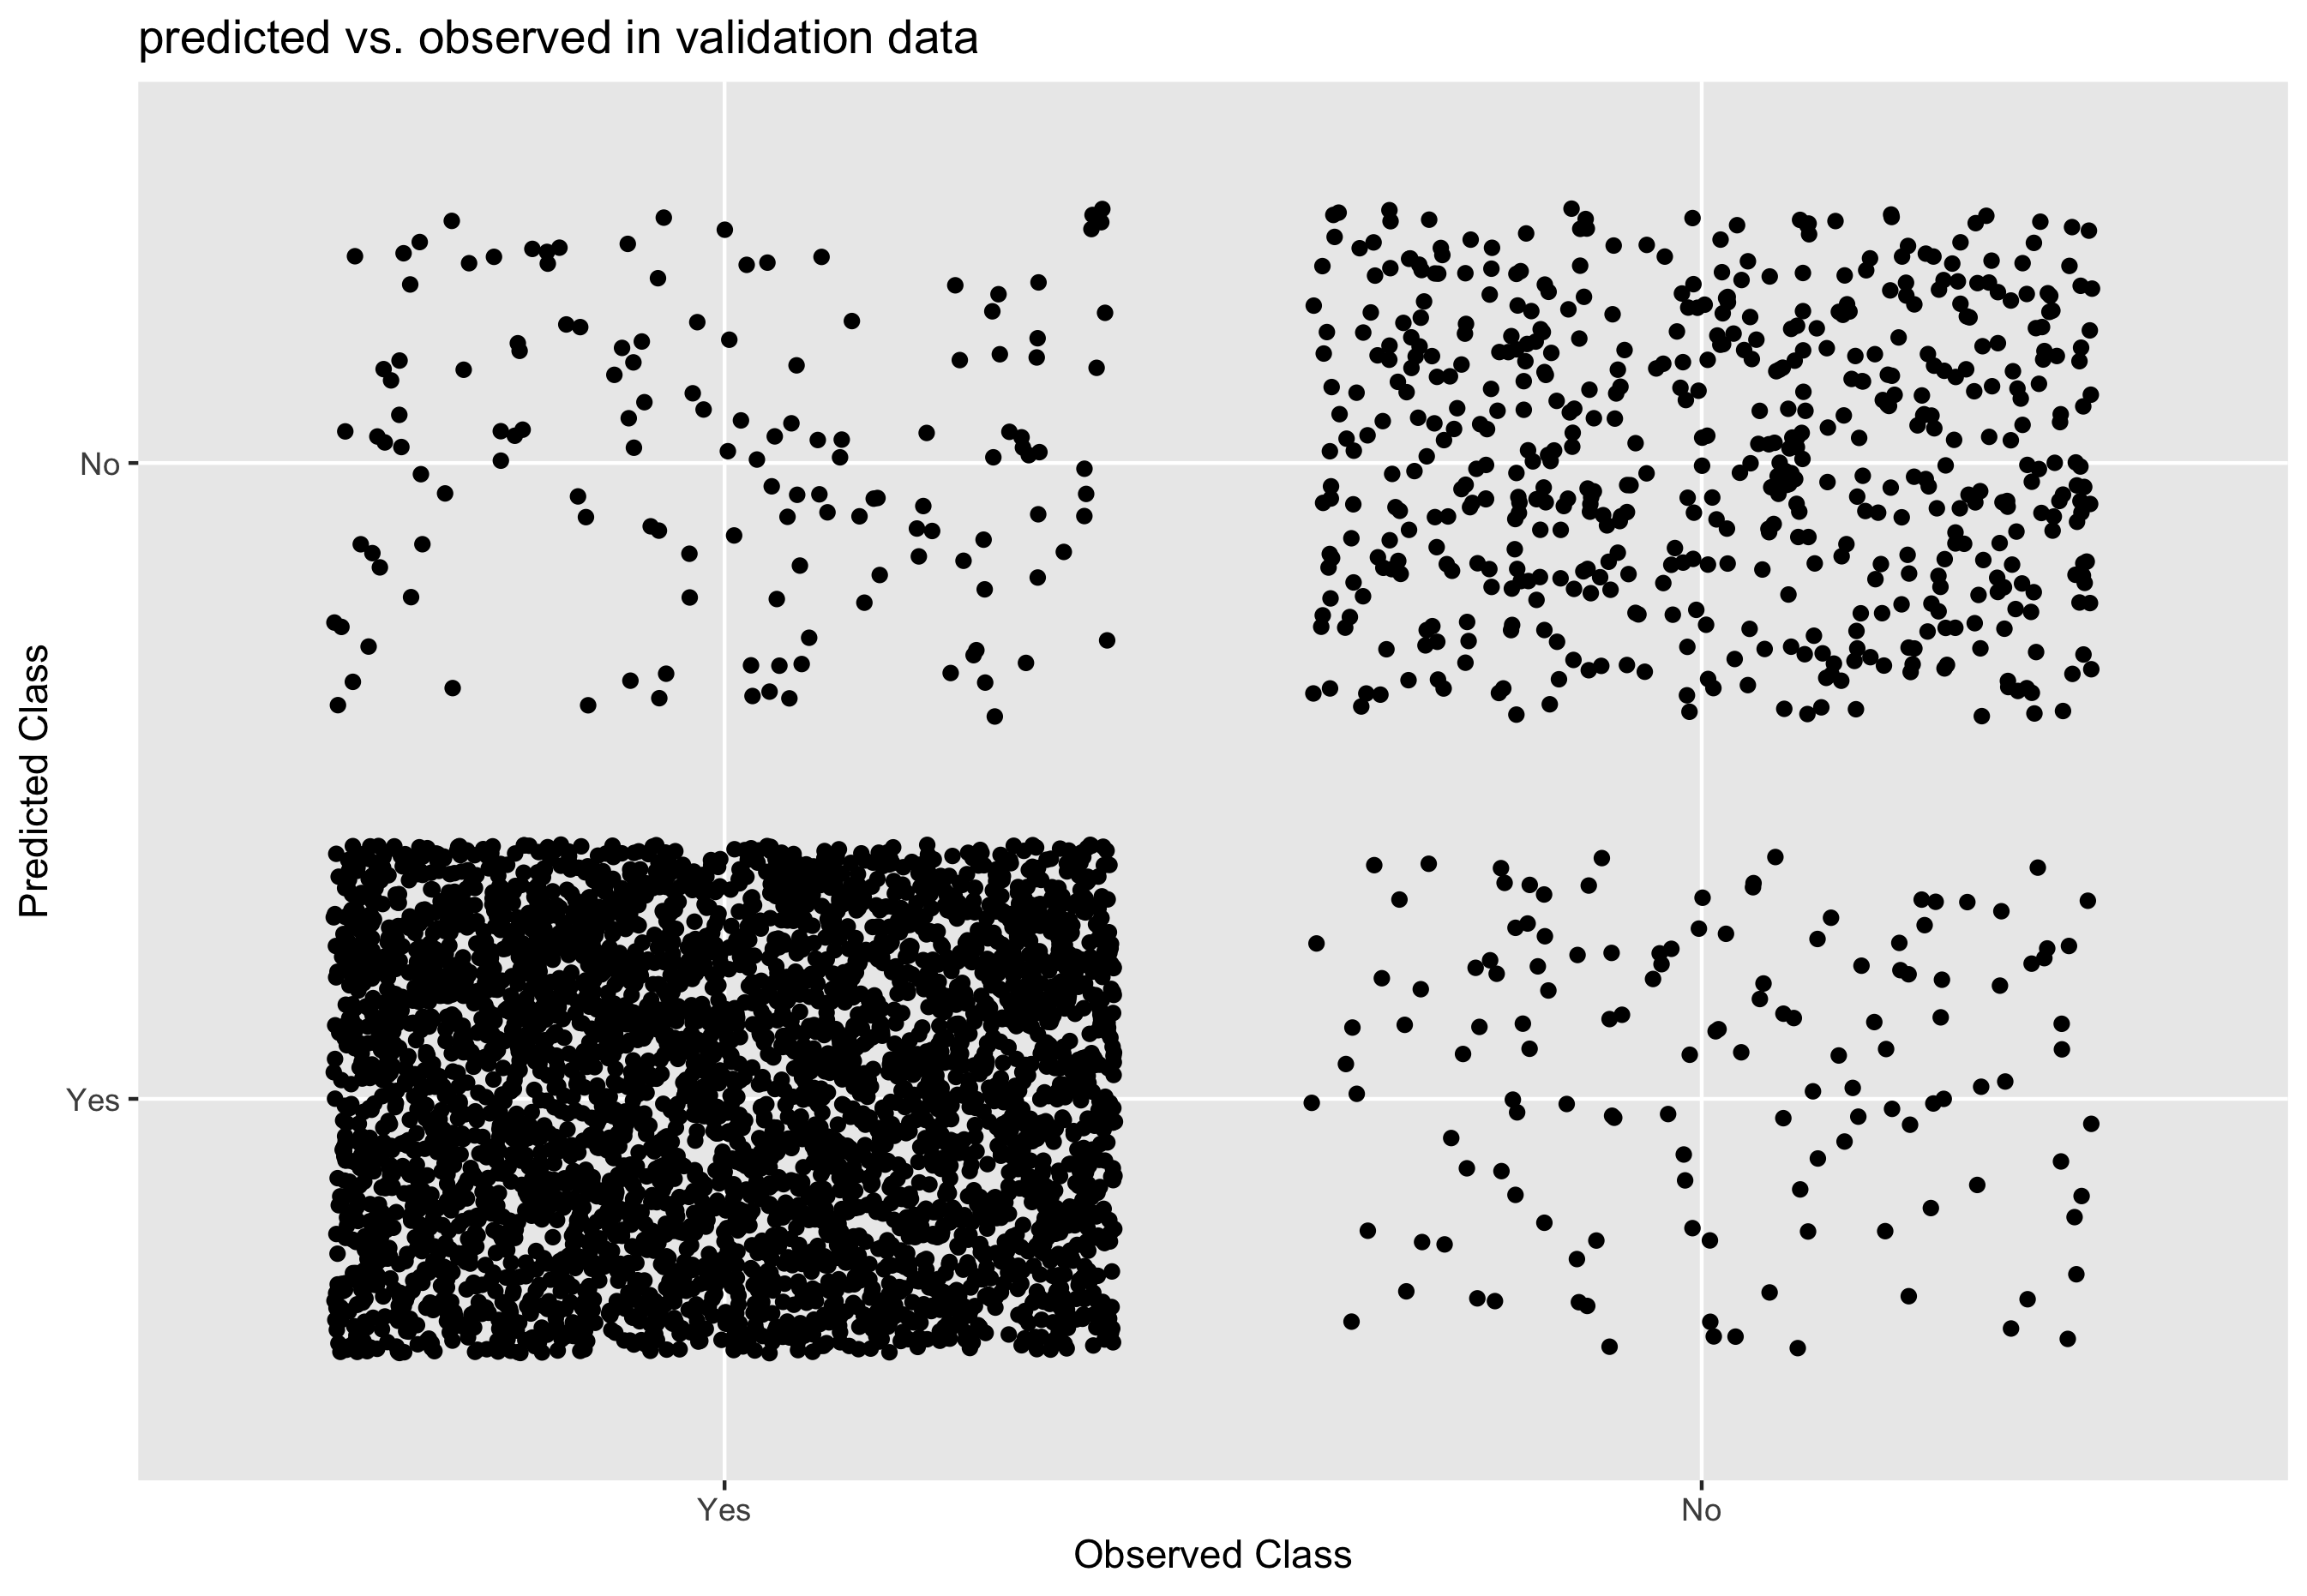
\includegraphics{images/STCANCEISqplot.png}
\caption{Performance of CANCEIS in predicting student status}
\end{figure}

\begin{figure}
\centering
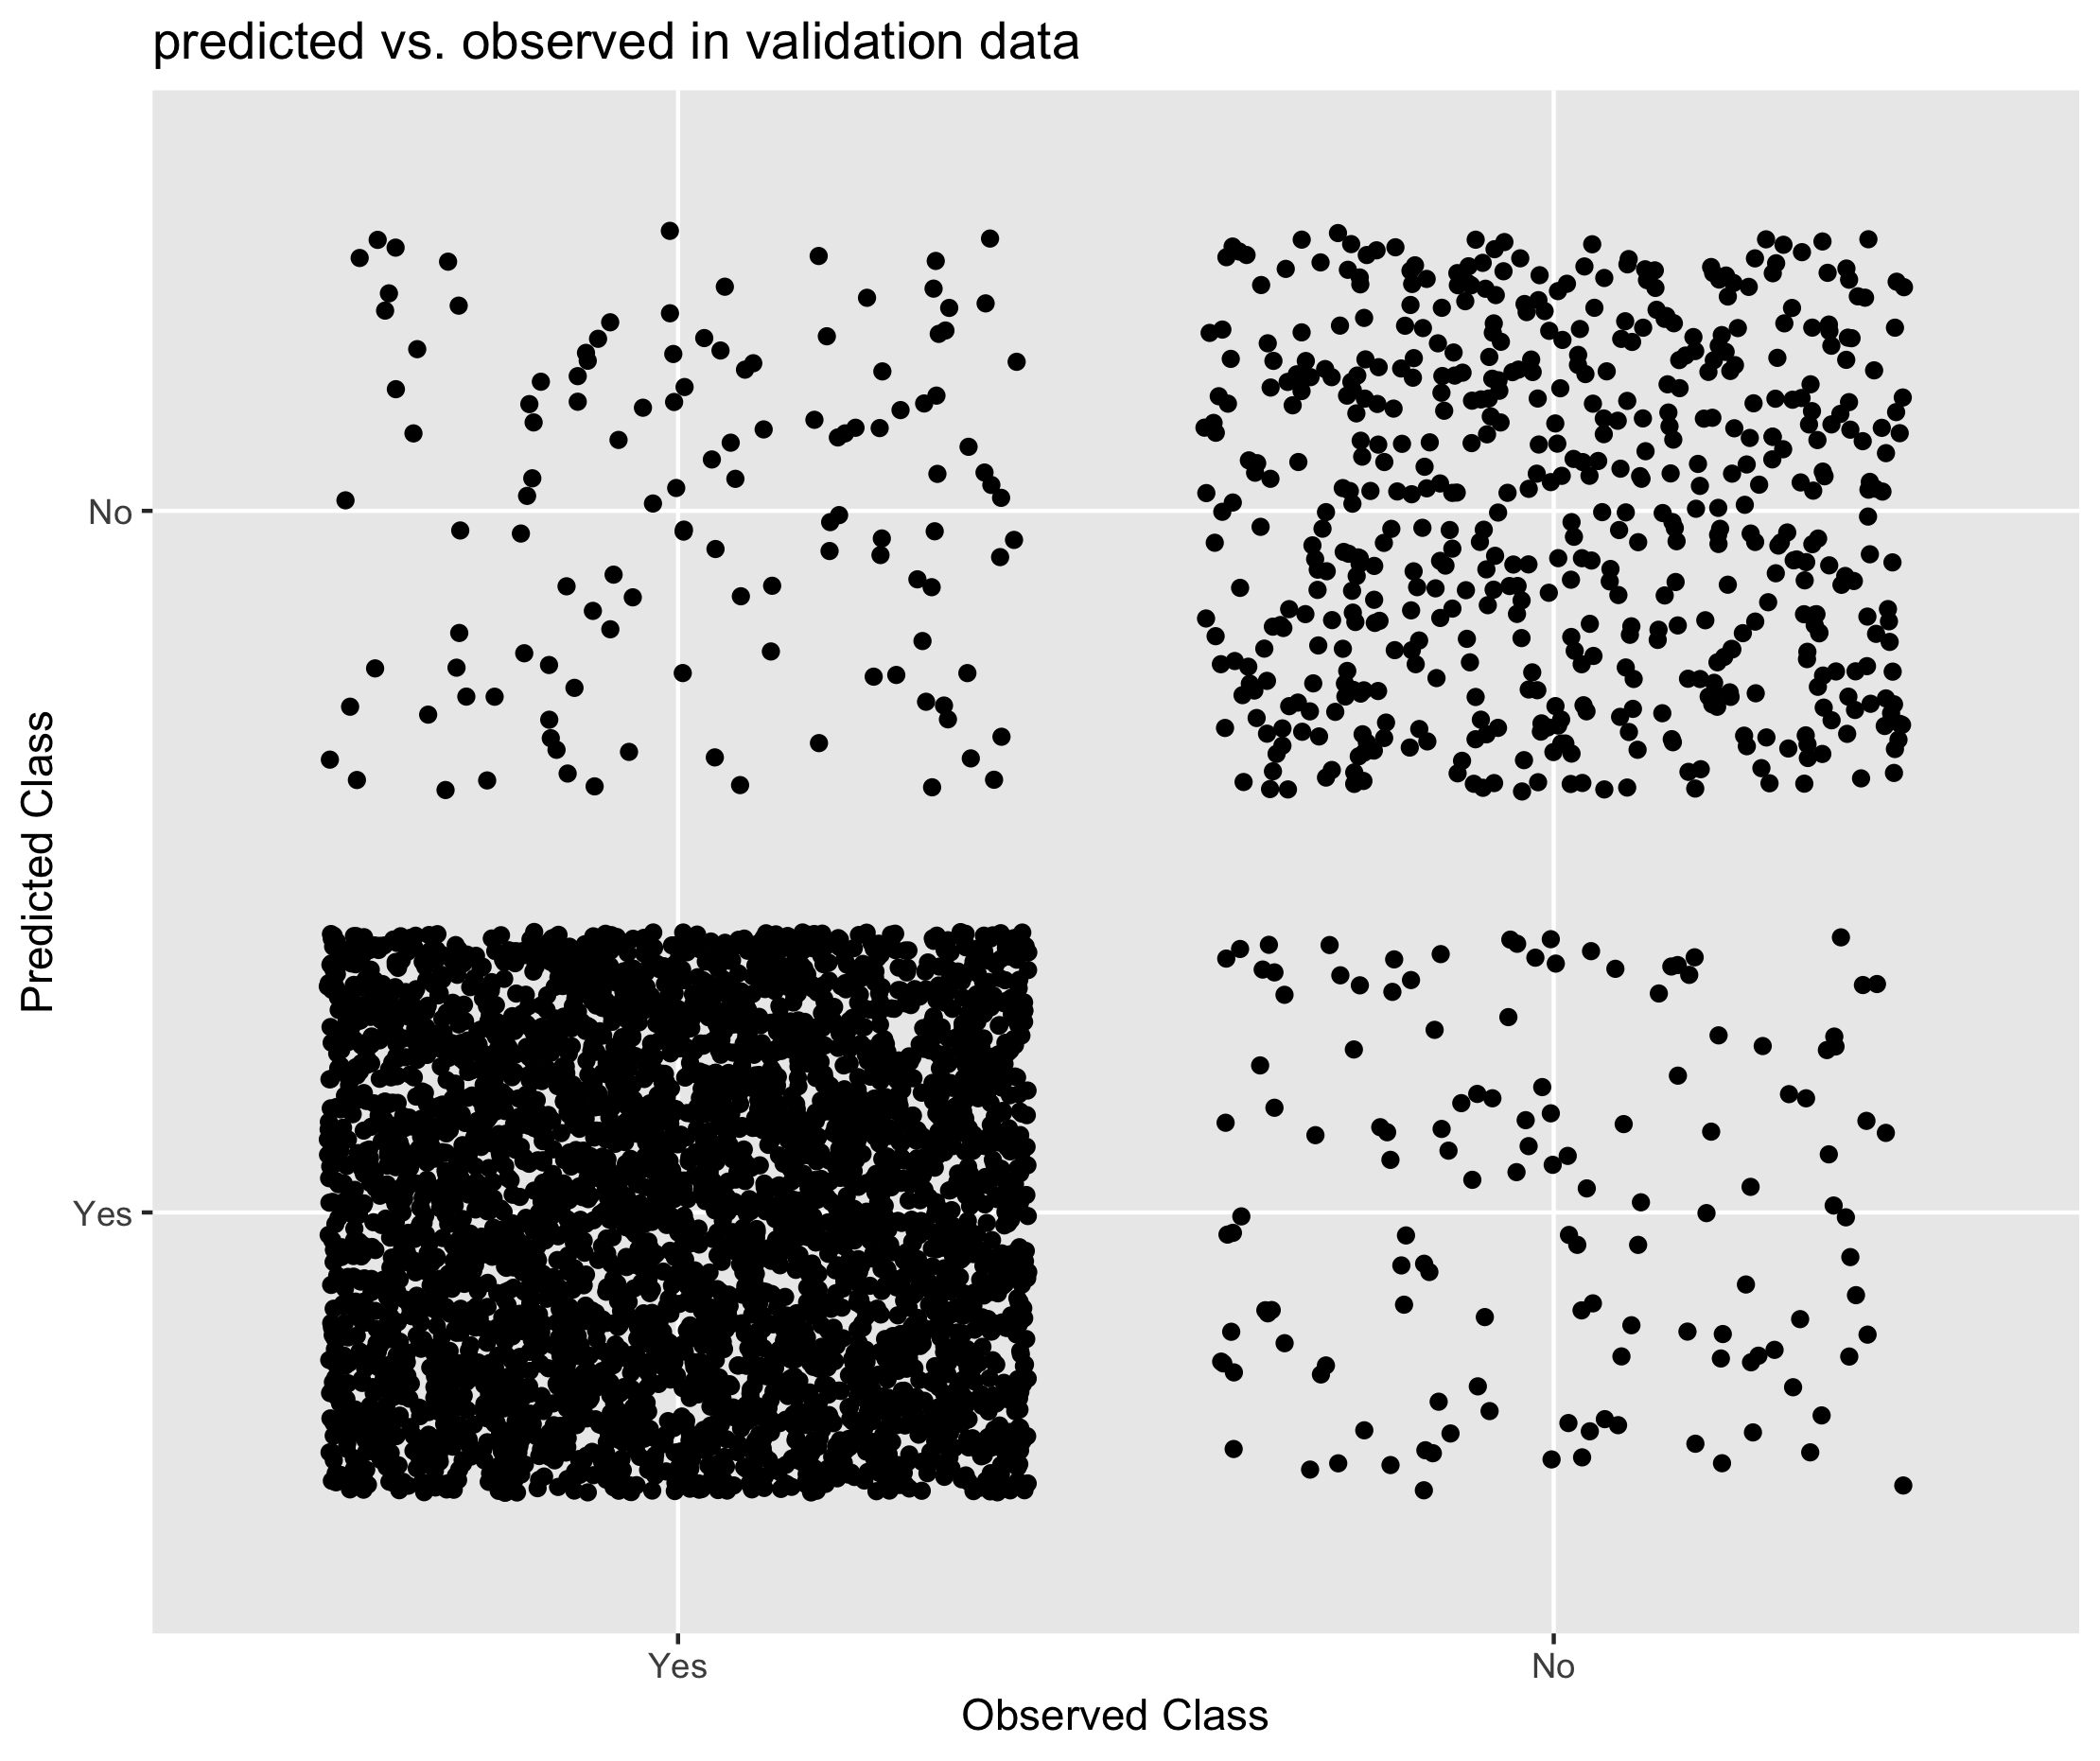
\includegraphics{images/STCANCEISXGqplot.png}
\caption{Performance of Mixed Methods approach in predicting student
status}
\end{figure}

\chapter{Next steps}\label{next-steps}

Preliminary results indicate that XGBoost performs well, relative to
donor based methods, in univariate imputation. The models were
especially effective at predicting the different classes of multi-class
and binary variables. The ability to program an end to end imputation
process is an added advantage of XGBoost; it reduces the time taken to
implement an imputation method, and presents clients with the option of
automating the imputation process. Current donor based methods utilise
either closed, or proprietary code, which cannot easily be integrated
into open source platforms.

The intention is to build on this work, and examine the efficacy of
machine learning systems on household survey imputation by carrying out
the following:

\begin{itemize}
\tightlist
\item
  Compare XGBoost, as well as Deep Learning methods (such as
  Autoencoders) to current donor based methods on ONS household survey
  data\\
\item
  Study how changes to XGBoost hyper-parameters can influence the
  performance of the imputation model. As the current investigation,
  using Census data, did not iterate through different combinations of
  hyper-parameters, it would be of interest to see if this improves the
  performance of this ML system in household survey imputation.\\
\item
  If time permits, it would be of interest to explore the use of XGBoost
  as a method to advise donor selection. That is, how the selection and
  importance of features could be used to identify matching variables
  and weights respectively.
\end{itemize}

\chapter{Resources}\label{resources}

\section{R scripts}\label{r-scripts}

All R scripts pertaining to this investigation are saved in the folder
``R''. If you are intending to run any of the code, please load all the
packages and functions first, which can be found in the script
``WF1\_package\_load.R'' and ``WF2\_function\_load.R''.

The program ``WF3\_data\_prep.R'' cleans and edits the data for the
investigation, whilst the scripts ``WF4\_missingness.R'' and
``WF5\_data\_load.R'' simulate missigness and produce descriptive
statistics of the data sets respectively. Scripts with the prefix
``WFI'' refer to programs that carry out the imputation for each
variable.

\section{Data}\label{data}

The folder named ``data'' includes:

\begin{itemize}
\tightlist
\item
  full Census Teaching File
\item
  test and training data
\item
  the predicted values from each imputation method and variable
\end{itemize}

\section{XGBoost}\label{xgboost-1}

The models produced for each imputable variable can be found in the
following folder (located in the main directory):

\begin{itemize}
\tightlist
\item
  XGBoost
\end{itemize}

\section{Donor imputation}\label{donor-imputation}

The CANCEIS specifications used for the two rounds of donor based
imputation can be found in the following folders (located in the main
directory):

\begin{itemize}
\tightlist
\item
  CANCEIS\\
\item
  MixedMethods
\end{itemize}

\bibliography{book.bib,packages.bib}


\end{document}
